
%% bare_adv.tex
%% V1.4b
%% 2015/08/26
%% by Michael Shell
%% See:
%% http://www.michaelshell.org/
%% for current contact information.
%%
%% This is a skeleton file demonstrating the advanced use of IEEEtran.cls
%% (requires IEEEtran.cls version 1.8b or later) with an IEEE Computer
%% Society journal paper.
%%
%% Support sites:
%% http://www.michaelshell.org/tex/ieeetran/
%% http://www.ctan.org/pkg/ieeetran
%% and
%% http://www.ieee.org/

%%*************************************************************************
%% Legal Notice:
%% This code is offered as-is without any warranty either expressed or
%% implied; without even the implied warranty of MERCHANTABILITY or
%% FITNESS FOR A PARTICULAR PURPOSE!
%% User assumes all risk.
%% In no event shall the IEEE or any contributor to this code be liable for
%% any damages or losses, including, but not limited to, incidental,
%% consequential, or any other damages, resulting from the use or misuse
%% of any information contained here.
%%
%% All comments are the opinions of their respective authors and are not
%% necessarily endorsed by the IEEE.
%%
%% This work is distributed under the LaTeX Project Public License (LPPL)
%% ( http://www.latex-project.org/ ) version 1.3, and may be freely used,
%% distributed and modified. A copy of the LPPL, version 1.3, is included
%% in the base LaTeX documentation of all distributions of LaTeX released
%% 2003/12/01 or later.
%% Retain all contribution notices and credits.
%% ** Modified files should be clearly indicated as such, including  **
%% ** renaming them and changing author support contact information. **
%%*************************************************************************


% *** Authors should verify (and, if needed, correct) their LaTeX system  ***
% *** with the testflow diagnostic prior to trusting their LaTeX platform ***
% *** with production work. The IEEE's font choices and paper sizes can   ***
% *** trigger bugs that do not appear when using other class files.       ***                          ***
% The testflow support page is at:
% http://www.michaelshell.org/tex/testflow/


% IEEEtran V1.7 and later provides for these CLASSINPUT macros to allow the
% user to reprogram some IEEEtran.cls defaults if needed. These settings
% override the internal defaults of IEEEtran.cls regardless of which class
% options are used. Do not use these unless you have good reason to do so as
% they can result in nonIEEE compliant documents. User beware. ;)
%
%\newcommand{\CLASSINPUTbaselinestretch}{1.0} % baselinestretch
%\newcommand{\CLASSINPUTinnersidemargin}{1in} % inner side margin
%\newcommand{\CLASSINPUToutersidemargin}{1in} % outer side margin
%\newcommand{\CLASSINPUTtoptextmargin}{1in}   % top text margin
%\newcommand{\CLASSINPUTbottomtextmargin}{1in}% bottom text margin




%
\documentclass[10pt,journal,compsoc]{IEEEtran}
% If IEEEtran.cls has not been installed into the LaTeX system files,
% manually specify the path to it like:
% \documentclass[10pt,journal,compsoc]{../sty/IEEEtran}


% For Computer Society journals, IEEEtran defaults to the use of
% Palatino/Palladio as is done in IEEE Computer Society journals.
% To go back to Times Roman, you can use this code:
%\renewcommand{\rmdefault}{ptm}\selectfont





% Some very useful LaTeX packages include:
% (uncomment the ones you want to load)



% *** MISC UTILITY PACKAGES ***
%
%\usepackage{ifpdf}
% Heiko Oberdiek's ifpdf.sty is very useful if you need conditional
% compilation based on whether the output is pdf or dvi.
% usage:
% \ifpdf
%   % pdf code
% \else
%   % dvi code
% \fi
% The latest version of ifpdf.sty can be obtained from:
% http://www.ctan.org/pkg/ifpdf
% Also, note that IEEEtran.cls V1.7 and later provides a builtin
% \ifCLASSINFOpdf conditional that works the same way.
% When switching from latex to pdflatex and vice-versa, the compiler may
% have to be run twice to clear warning/error messages.






% *** CITATION PACKAGES ***
%
\ifCLASSOPTIONcompsoc
  % The IEEE Computer Society needs nocompress option
  % requires cite.sty v4.0 or later (November 2003)
  \usepackage[nocompress]{cite}
\else
  % normal IEEE
  \usepackage{cite}
\fi

\usepackage[utf8]{inputenc} % allow utf-8 input
\usepackage[T1]{fontenc}    % use 8-bit T1 fonts
\usepackage{hyperref}       % hyperlinks
\usepackage{url}            % simple URL typesetting
\usepackage{booktabs}       % professional-quality tables
\usepackage{amsfonts}       % blackboard math symbols
\usepackage{nicefrac}       % compact symbols for 1/2, etc.
\usepackage{microtype}      % microtypography
\usepackage{graphicx,float,url,multirow,makecell,booktabs,color,subfigure,caption,setspace}
\usepackage{amsmath}
\usepackage{cite}
\usepackage{psfrag}
\usepackage{epsfig,latexsym}
\usepackage{times}
\usepackage{epsfig}
\usepackage{graphicx}
\usepackage{amsmath}
\usepackage{amssymb}
\usepackage{graphicx}
\usepackage{epstopdf}
% For algorithms
\usepackage{algorithm}
\usepackage{algorithmic}


\newcommand{\argmin}{\operatornamewithlimits{argmin}}
\newcommand{\argmax}{\operatornamewithlimits{argmax}}

\newcommand{\tabincell}[2]{\begin{tabular}{@{}#1@{}}#2\end{tabular}}

\newtheorem{theorem}{$\textbf{Theorem}$}
\newtheorem{lemma}[theorem]{$\textbf{Lemma}$}
\newtheorem{proposition}[theorem]{$\textbf{Proposition}$}

% Strut macros for skipping spaces above and below text in tables.
\def\abovestrut#1{\rule[0in]{0in}{#1}\ignorespaces}
\def\belowstrut#1{\rule[-#1]{0in}{#1}\ignorespaces}
\def\abovespace{\abovestrut{0.01in}}
\def\belowspace{\belowstrut{-0.01in}}
% cite.sty was written by Donald Arseneau
% V1.6 and later of IEEEtran pre-defines the format of the cite.sty package
% \cite{} output to follow that of the IEEE. Loading the cite package will
% result in citation numbers being automatically sorted and properly
% "compressed/ranged". e.g., [1], [9], [2], [7], [5], [6] without using
% cite.sty will become [1], [2], [5]--[7], [9] using cite.sty. cite.sty's
% \cite will automatically add leading space, if needed. Use cite.sty's
% noadjust option (cite.sty V3.8 and later) if you want to turn this off
% such as if a citation ever needs to be enclosed in parenthesis.
% cite.sty is already installed on most LaTeX systems. Be sure and use
% version 5.0 (2009-03-20) and later if using hyperref.sty.
% The latest version can be obtained at:
% http://www.ctan.org/pkg/cite
% The documentation is contained in the cite.sty file itself.
%
% Note that some packages require special options to format as the Computer
% Society requires. In particular, Computer Society  papers do not use
% compressed citation ranges as is done in typical IEEE papers
% (e.g., [1]-[4]). Instead, they list every citation separately in order
% (e.g., [1], [2], [3], [4]). To get the latter we need to load the cite
% package with the nocompress option which is supported by cite.sty v4.0
% and later.





% *** GRAPHICS RELATED PACKAGES ***
%
\ifCLASSINFOpdf
  % \usepackage[pdftex]{graphicx}
  % declare the path(s) where your graphic files are
  % \graphicspath{{../pdf/}{../jpeg/}}
  % and their extensions so you won't have to specify these with
  % every instance of \includegraphics
  % \DeclareGraphicsExtensions{.pdf,.jpeg,.png}
\else
  % or other class option (dvipsone, dvipdf, if not using dvips). graphicx
  % will default to the driver specified in the system graphics.cfg if no
  % driver is specified.
  % \usepackage[dvips]{graphicx}
  % declare the path(s) where your graphic files are
  % \graphicspath{{../eps/}}
  % and their extensions so you won't have to specify these with
  % every instance of \includegraphics
  % \DeclareGraphicsExtensions{.eps}
\fi
% graphicx was written by David Carlisle and Sebastian Rahtz. It is
% required if you want graphics, photos, etc. graphicx.sty is already
% installed on most LaTeX systems. The latest version and documentation
% can be obtained at:
% http://www.ctan.org/pkg/graphicx
% Another good source of documentation is "Using Imported Graphics in
% LaTeX2e" by Keith Reckdahl which can be found at:
% http://www.ctan.org/pkg/epslatex
%
% latex, and pdflatex in dvi mode, support graphics in encapsulated
% postscript (.eps) format. pdflatex in pdf mode supports graphics
% in .pdf, .jpeg, .png and .mps (metapost) formats. Users should ensure
% that all non-photo figures use a vector format (.eps, .pdf, .mps) and
% not a bitmapped formats (.jpeg, .png). The IEEE frowns on bitmapped formats
% which can result in "jaggedy"/blurry rendering of lines and letters as
% well as large increases in file sizes.
%
% You can find documentation about the pdfTeX application at:
% http://www.tug.org/applications/pdftex





% *** MATH PACKAGES ***
%
%\usepackage{amsmath}
% A popular package from the American Mathematical Society that provides
% many useful and powerful commands for dealing with mathematics.
%
% Note that the amsmath package sets \interdisplaylinepenalty to 10000
% thus preventing page breaks from occurring within multiline equations. Use:
%\interdisplaylinepenalty=2500
% after loading amsmath to restore such page breaks as IEEEtran.cls normally
% does. amsmath.sty is already installed on most LaTeX systems. The latest
% version and documentation can be obtained at:
% http://www.ctan.org/pkg/amsmath





% *** SPECIALIZED LIST PACKAGES ***
%\usepackage{acronym}
% acronym.sty was written by Tobias Oetiker. This package provides tools for
% managing documents with large numbers of acronyms. (You don't *have* to
% use this package - unless you have a lot of acronyms, you may feel that
% such package management of them is bit of an overkill.)
% Do note that the acronym environment (which lists acronyms) will have a
% problem when used under IEEEtran.cls because acronym.sty relies on the
% description list environment - which IEEEtran.cls has customized for
% producing IEEE style lists. A workaround is to declared the longest
% label width via the IEEEtran.cls \IEEEiedlistdecl global control:
%
% \renewcommand{\IEEEiedlistdecl}{\IEEEsetlabelwidth{SONET}}
% \begin{acronym}
%
% \end{acronym}
% \renewcommand{\IEEEiedlistdecl}{\relax}% remember to reset \IEEEiedlistdecl
%
% instead of using the acronym environment's optional argument.
% The latest version and documentation can be obtained at:
% http://www.ctan.org/pkg/acronym


%\usepackage{algorithmic}
% algorithmic.sty was written by Peter Williams and Rogerio Brito.
% This package provides an algorithmic environment fo describing algorithms.
% You can use the algorithmic environment in-text or within a figure
% environment to provide for a floating algorithm. Do NOT use the algorithm
% floating environment provided by algorithm.sty (by the same authors) or
% algorithm2e.sty (by Christophe Fiorio) as the IEEE does not use dedicated
% algorithm float types and packages that provide these will not provide
% correct IEEE style captions. The latest version and documentation of
% algorithmic.sty can be obtained at:
% http://www.ctan.org/pkg/algorithms
% Also of interest may be the (relatively newer and more customizable)
% algorithmicx.sty package by Szasz Janos:
% http://www.ctan.org/pkg/algorithmicx




% *** ALIGNMENT PACKAGES ***
%
%\usepackage{array}
% Frank Mittelbach's and David Carlisle's array.sty patches and improves
% the standard LaTeX2e array and tabular environments to provide better
% appearance and additional user controls. As the default LaTeX2e table
% generation code is lacking to the point of almost being broken with
% respect to the quality of the end results, all users are strongly
% advised to use an enhanced (at the very least that provided by array.sty)
% set of table tools. array.sty is already installed on most systems. The
% latest version and documentation can be obtained at:
% http://www.ctan.org/pkg/array


%\usepackage{mdwmath}
%\usepackage{mdwtab}
% Also highly recommended is Mark Wooding's extremely powerful MDW tools,
% especially mdwmath.sty and mdwtab.sty which are used to format equations
% and tables, respectively. The MDWtools set is already installed on most
% LaTeX systems. The lastest version and documentation is available at:
% http://www.ctan.org/pkg/mdwtools


% IEEEtran contains the IEEEeqnarray family of commands that can be used to
% generate multiline equations as well as matrices, tables, etc., of high
% quality.


%\usepackage{eqparbox}
% Also of notable interest is Scott Pakin's eqparbox package for creating
% (automatically sized) equal width boxes - aka "natural width parboxes".
% Available at:
% http://www.ctan.org/pkg/eqparbox




% *** SUBFIGURE PACKAGES ***
%\ifCLASSOPTIONcompsoc
%  \usepackage[caption=false,font=footnotesize,labelfont=sf,textfont=sf]{subfig}
%\else
%  \usepackage[caption=false,font=footnotesize]{subfig}
%\fi
% subfig.sty, written by Steven Douglas Cochran, is the modern replacement
% for subfigure.sty, the latter of which is no longer maintained and is
% incompatible with some LaTeX packages including fixltx2e. However,
% subfig.sty requires and automatically loads Axel Sommerfeldt's caption.sty
% which will override IEEEtran.cls' handling of captions and this will result
% in non-IEEE style figure/table captions. To prevent this problem, be sure
% and invoke subfig.sty's "caption=false" package option (available since
% subfig.sty version 1.3, 2005/06/28) as this is will preserve IEEEtran.cls
% handling of captions.
% Note that the Computer Society format requires a sans serif font rather
% than the serif font used in traditional IEEE formatting and thus the need
% to invoke different subfig.sty package options depending on whether
% compsoc mode has been enabled.
%
% The latest version and documentation of subfig.sty can be obtained at:
% http://www.ctan.org/pkg/subfig




% *** FLOAT PACKAGES ***
%
%\usepackage{fixltx2e}
% fixltx2e, the successor to the earlier fix2col.sty, was written by
% Frank Mittelbach and David Carlisle. This package corrects a few problems
% in the LaTeX2e kernel, the most notable of which is that in current
% LaTeX2e releases, the ordering of single and double column floats is not
% guaranteed to be preserved. Thus, an unpatched LaTeX2e can allow a
% single column figure to be placed prior to an earlier double column
% figure.
% Be aware that LaTeX2e kernels dated 2015 and later have fixltx2e.sty's
% corrections already built into the system in which case a warning will
% be issued if an attempt is made to load fixltx2e.sty as it is no longer
% needed.
% The latest version and documentation can be found at:
% http://www.ctan.org/pkg/fixltx2e


%\usepackage{stfloats}
% stfloats.sty was written by Sigitas Tolusis. This package gives LaTeX2e
% the ability to do double column floats at the bottom of the page as well
% as the top. (e.g., "\begin{figure*}[!b]" is not normally possible in
% LaTeX2e). It also provides a command:
%\fnbelowfloat
% to enable the placement of footnotes below bottom floats (the standard
% LaTeX2e kernel puts them above bottom floats). This is an invasive package
% which rewrites many portions of the LaTeX2e float routines. It may not work
% with other packages that modify the LaTeX2e float routines. The latest
% version and documentation can be obtained at:
% http://www.ctan.org/pkg/stfloats
% Do not use the stfloats baselinefloat ability as the IEEE does not allow
% \baselineskip to stretch. Authors submitting work to the IEEE should note
% that the IEEE rarely uses double column equations and that authors should try
% to avoid such use. Do not be tempted to use the cuted.sty or midfloat.sty
% packages (also by Sigitas Tolusis) as the IEEE does not format its papers in
% such ways.
% Do not attempt to use stfloats with fixltx2e as they are incompatible.
% Instead, use Morten Hogholm'a dblfloatfix which combines the features
% of both fixltx2e and stfloats:
%
% \usepackage{dblfloatfix}
% The latest version can be found at:
% http://www.ctan.org/pkg/dblfloatfix


%\ifCLASSOPTIONcaptionsoff
%  \usepackage[nomarkers]{endfloat}
% \let\MYoriglatexcaption\caption
% \renewcommand{\caption}[2][\relax]{\MYoriglatexcaption[#2]{#2}}
%\fi
% endfloat.sty was written by James Darrell McCauley, Jeff Goldberg and
% Axel Sommerfeldt. This package may be useful when used in conjunction with
% IEEEtran.cls'  captionsoff option. Some IEEE journals/societies require that
% submissions have lists of figures/tables at the end of the paper and that
% figures/tables without any captions are placed on a page by themselves at
% the end of the document. If needed, the draftcls IEEEtran class option or
% \CLASSINPUTbaselinestretch interface can be used to increase the line
% spacing as well. Be sure and use the nomarkers option of endfloat to
% prevent endfloat from "marking" where the figures would have been placed
% in the text. The two hack lines of code above are a slight modification of
% that suggested by in the endfloat docs (section 8.4.1) to ensure that
% the full captions always appear in the list of figures/tables - even if
% the user used the short optional argument of \caption[]{}.
% IEEE papers do not typically make use of \caption[]'s optional argument,
% so this should not be an issue. A similar trick can be used to disable
% captions of packages such as subfig.sty that lack options to turn off
% the subcaptions:
% For subfig.sty:
% \let\MYorigsubfloat\subfloat
% \renewcommand{\subfloat}[2][\relax]{\MYorigsubfloat[]{#2}}
% However, the above trick will not work if both optional arguments of
% the \subfloat command are used. Furthermore, there needs to be a
% description of each subfigure *somewhere* and endfloat does not add
% subfigure captions to its list of figures. Thus, the best approach is to
% avoid the use of subfigure captions (many IEEE journals avoid them anyway)
% and instead reference/explain all the subfigures within the main caption.
% The latest version of endfloat.sty and its documentation can obtained at:
% http://www.ctan.org/pkg/endfloat
%
% The IEEEtran \ifCLASSOPTIONcaptionsoff conditional can also be used
% later in the document, say, to conditionally put the References on a
% page by themselves.





% *** PDF, URL AND HYPERLINK PACKAGES ***
%
%\usepackage{url}
% url.sty was written by Donald Arseneau. It provides better support for
% handling and breaking URLs. url.sty is already installed on most LaTeX
% systems. The latest version and documentation can be obtained at:
% http://www.ctan.org/pkg/url
% Basically, \url{my_url_here}.


% NOTE: PDF thumbnail features are not required in IEEE papers
%       and their use requires extra complexity and work.
%\ifCLASSINFOpdf
%  \usepackage[pdftex]{thumbpdf}
%\else
%  \usepackage[dvips]{thumbpdf}
%\fi
% thumbpdf.sty and its companion Perl utility were written by Heiko Oberdiek.
% It allows the user a way to produce PDF documents that contain fancy
% thumbnail images of each of the pages (which tools like acrobat reader can
% utilize). This is possible even when using dvi->ps->pdf workflow if the
% correct thumbpdf driver options are used. thumbpdf.sty incorporates the
% file containing the PDF thumbnail information (filename.tpm is used with
% dvips, filename.tpt is used with pdftex, where filename is the base name of
% your tex document) into the final ps or pdf output document. An external
% utility, the thumbpdf *Perl script* is needed to make these .tpm or .tpt
% thumbnail files from a .ps or .pdf version of the document (which obviously
% does not yet contain pdf thumbnails). Thus, one does a:
%
% thumbpdf filename.pdf
%
% to make a filename.tpt, and:
%
% thumbpdf --mode dvips filename.ps
%
% to make a filename.tpm which will then be loaded into the document by
% thumbpdf.sty the NEXT time the document is compiled (by pdflatex or
% latex->dvips->ps2pdf). Users must be careful to regenerate the .tpt and/or
% .tpm files if the main document changes and then to recompile the
% document to incorporate the revised thumbnails to ensure that thumbnails
% match the actual pages. It is easy to forget to do this!
%
% Unix systems come with a Perl interpreter. However, MS Windows users
% will usually have to install a Perl interpreter so that the thumbpdf
% script can be run. The Ghostscript PS/PDF interpreter is also required.
% See the thumbpdf docs for details. The latest version and documentation
% can be obtained at.
% http://www.ctan.org/pkg/thumbpdf


% NOTE: PDF hyperlink and bookmark features are not required in IEEE
%       papers and their use requires extra complexity and work.
% *** IF USING HYPERREF BE SURE AND CHANGE THE EXAMPLE PDF ***
% *** TITLE/SUBJECT/AUTHOR/KEYWORDS INFO BELOW!!           ***
\newcommand\MYhyperrefoptions{bookmarks=true,bookmarksnumbered=true,
pdfpagemode={UseOutlines},plainpages=false,pdfpagelabels=true,
colorlinks=true,linkcolor={black},citecolor={black},urlcolor={black},
pdftitle={Bare Demo of IEEEtran.cls for Computer Society Journals},%<!CHANGE!
pdfsubject={Typesetting},%<!CHANGE!
pdfauthor={Michael D. Shell},%<!CHANGE!
pdfkeywords={Computer Society, IEEEtran, journal, LaTeX, paper,
             template}}%<^!CHANGE!
%\ifCLASSINFOpdf
%\usepackage[\MYhyperrefoptions,pdftex]{hyperref}
%\else
%\usepackage[\MYhyperrefoptions,breaklinks=true,dvips]{hyperref}
%\usepackage{breakurl}
%\fi
% One significant drawback of using hyperref under DVI output is that the
% LaTeX compiler cannot break URLs across lines or pages as can be done
% under pdfLaTeX's PDF output via the hyperref pdftex driver. This is
% probably the single most important capability distinction between the
% DVI and PDF output. Perhaps surprisingly, all the other PDF features
% (PDF bookmarks, thumbnails, etc.) can be preserved in
% .tex->.dvi->.ps->.pdf workflow if the respective packages/scripts are
% loaded/invoked with the correct driver options (dvips, etc.).
% As most IEEE papers use URLs sparingly (mainly in the references), this
% may not be as big an issue as with other publications.
%
% That said, Vilar Camara Neto created his breakurl.sty package which
% permits hyperref to easily break URLs even in dvi mode.
% Note that breakurl, unlike most other packages, must be loaded
% AFTER hyperref. The latest version of breakurl and its documentation can
% be obtained at:
% http://www.ctan.org/pkg/breakurl
% breakurl.sty is not for use under pdflatex pdf mode.
%
% The advanced features offer by hyperref.sty are not required for IEEE
% submission, so users should weigh these features against the added
% complexity of use.
% The package options above demonstrate how to enable PDF bookmarks
% (a type of table of contents viewable in Acrobat Reader) as well as
% PDF document information (title, subject, author and keywords) that is
% viewable in Acrobat reader's Document_Properties menu. PDF document
% information is also used extensively to automate the cataloging of PDF
% documents. The above set of options ensures that hyperlinks will not be
% colored in the text and thus will not be visible in the printed page,
% but will be active on "mouse over". USING COLORS OR OTHER HIGHLIGHTING
% OF HYPERLINKS CAN RESULT IN DOCUMENT REJECTION BY THE IEEE, especially if
% these appear on the "printed" page. IF IN DOUBT, ASK THE RELEVANT
% SUBMISSION EDITOR. You may need to add the option hypertexnames=false if
% you used duplicate equation numbers, etc., but this should not be needed
% in normal IEEE work.
% The latest version of hyperref and its documentation can be obtained at:
% http://www.ctan.org/pkg/hyperref





% *** Do not adjust lengths that control margins, column widths, etc. ***
% *** Do not use packages that alter fonts (such as pslatex).         ***
% There should be no need to do such things with IEEEtran.cls V1.6 and later.
% (Unless specifically asked to do so by the journal or conference you plan
% to submit to, of course. )


% correct bad hyphenation here
\hyphenation{op-tical net-works semi-conduc-tor}


\begin{document}
%
% paper title
% Titles are generally capitalized except for words such as a, an, and, as,
% at, but, by, for, in, nor, of, on, or, the, to and up, which are usually
% not capitalized unless they are the first or last word of the title.
% Linebreaks \\ can be used within to get better formatting as desired.
% Do not put math or special symbols in the title.
\title{Modeling Attention in Panoramic Video: \\A Reinforcement Learning Approach}
%
%
% author names and IEEE memberships
% note positions of commas and nonbreaking spaces ( ~ ) LaTeX will not break
% a structure at a ~ so this keeps an author's name from being broken across
% two lines.
% use \thanks{} to gain access to the first footnote area
% a separate \thanks must be used for each paragraph as LaTeX2e's \thanks
% was not built to handle multiple paragraphs
%
%
%\IEEEcompsocitemizethanks is a special \thanks that produces the bulleted
% lists the Computer Society journals use for "first footnote" author
% affiliations. Use \IEEEcompsocthanksitem which works much like \item
% for each affiliation group. When not in compsoc mode,
% \IEEEcompsocitemizethanks becomes like \thanks and
% \IEEEcompsocthanksitem becomes a line break with idention. This
% facilitates dual compilation, although admittedly the differences in the
% desired content of \author between the different types of papers makes a
% one-size-fits-all approach a daunting prospect. For instance, compsoc
% journal papers have the author affiliations above the "Manuscript
% received ..."  text while in non-compsoc journals this is reversed. Sigh.

\author{Mai~Xu*,~\IEEEmembership{Senior Member,~IEEE,}
        Yuhang~Song*, Jianyi Wang, Minglang~Qiao, Liangyu Huo
        and~Haochen~Wang% <-this % stops a space
\IEEEcompsocitemizethanks{\IEEEcompsocthanksitem  M. Xu, Y. Song, J. Wang, M. Qiao, L. Huo and H. Wang are with the School of Electronic and Information
Engineering, Beihang University, Beijing, 100191 China\protect\\
% note need leading \protect in front of \\ to get a newline within \thanks as
% \\ is fragile and will error, could use \hfil\break instead.
E-mail: MaiXu@buaa.edu.cn
\IEEEcompsocthanksitem M. Xu and Y. Song contribute equality to this work.}% <-this % stops a space
\thanks{Manuscript received Oct 1, 2017; revised Dec 30, 2017.}}

% note the % following the last \IEEEmembership and also \thanks -
% these prevent an unwanted space from occurring between the last author name
% and the end of the author line. i.e., if you had this:
%
% \author{....lastname \thanks{...} \thanks{...} }
%                     ^------------^------------^----Do not want these spaces!
%
% a space would be appended to the last name and could cause every name on that
% line to be shifted left slightly. This is one of those "LaTeX things". For
% instance, "\textbf{A} \textbf{B}" will typeset as "A B" not "AB". To get
% "AB" then you have to do: "\textbf{A}\textbf{B}"
% \thanks is no different in this regard, so shield the last } of each \thanks
% that ends a line with a % and do not let a space in before the next \thanks.
% Spaces after \IEEEmembership other than the last one are OK (and needed) as
% you are supposed to have spaces between the names. For what it is worth,
% this is a minor point as most people would not even notice if the said evil
% space somehow managed to creep in.



% The paper headers
\markboth{Journal of \LaTeX\ Class Files,~Vol.~14, No.~8, August~2015}%
{Shell \MakeLowercase{\textit{et al.}}: Bare Advanced Demo of IEEEtran.cls for IEEE Computer Society Journals}
% The only time the second header will appear is for the odd numbered pages
% after the title page when using the twoside option.
%
% *** Note that you probably will NOT want to include the author's ***
% *** name in the headers of peer review papers.                   ***
% You can use \ifCLASSOPTIONpeerreview for conditional compilation here if
% you desire.



% The publisher's ID mark at the bottom of the page is less important with
% Computer Society journal papers as those publications place the marks
% outside of the main text columns and, therefore, unlike regular IEEE
% journals, the available text space is not reduced by their presence.
% If you want to put a publisher's ID mark on the page you can do it like
% this:
%\IEEEpubid{0000--0000/00\$00.00~\copyright~2015 IEEE}
% or like this to get the Computer Society new two part style.
%\IEEEpubid{\makebox[\columnwidth]{\hfill 0000--0000/00/\$00.00~\copyright~2015 IEEE}%
%\hspace{\columnsep}\makebox[\columnwidth]{Published by the IEEE Computer Society\hfill}}
% Remember, if you use this you must call \IEEEpubidadjcol in the second
% column for its text to clear the IEEEpubid mark (Computer Society journal
% papers don't need this extra clearance.)



% use for special paper notices
%\IEEEspecialpapernotice{(Invited Paper)}



% for Computer Society papers, we must declare the abstract and index terms
% PRIOR to the title within the \IEEEtitleabstractindextext IEEEtran
% command as these need to go into the title area created by \maketitle.
% As a general rule, do not put math, special symbols or citations
% in the abstract or keywords.
\IEEEtitleabstractindextext{%
\begin{abstract}
Panoramic video provides an immersive and interactive experience by enabling humans to control the field of view (FoV) through head movement (HM).
Thus, HM plays a key role in modeling human attention on panoramic video.
This paper establishes a database collecting subjects' HM positions on panoramic video sequences. From this database, we find that the HM data are highly consistent across subjects. Furthermore, we find that deep reinforcement learning (DRL) can be applied to predict HM positions, via maximizing the reward of imitating human HM scanpaths through the agent's actions.
Based on our findings, we propose a DRL based HM prediction (DHP) approach with offline and online versions, called offline-DHP and online-DHP, respectively.
In offline-DHP, multiple DRL workflows are run to determine some potential HM positions at each panoramic frame.
Then, a heat map of the potential HM positions, called the HM map, is generated as the output of offline-DHP.
In online-DHP, the next HM position of one subject is estimated given the currently observed HM position.
Online-DHP is achieved by developing a DRL algorithm, upon the learned model of offline-DHP.
Finally, the experimental results validate that the offline-DHP and online-DHP are effective in offline and online prediction of HM positions for panoramic video, and that the learned offline-DHP model can improve the performance of online-DHP.
\end{abstract}

% Note that keywords are not normally used for peerreview papers.
\begin{IEEEkeywords}
Panoramic video, head movement, reinforcement learning, deep learning.
\end{IEEEkeywords}}


% make the title area
\maketitle


% To allow for easy dual compilation without having to reenter the
% abstract/keywords data, the \IEEEtitleabstractindextext text will
% not be used in maketitle, but will appear (i.e., to be "transported")
% here as \IEEEdisplaynontitleabstractindextext when compsoc mode
% is not selected <OR> if conference mode is selected - because compsoc
% conference papers position the abstract like regular (non-compsoc)
% papers do!
\IEEEdisplaynontitleabstractindextext
% \IEEEdisplaynontitleabstractindextext has no effect when using
% compsoc under a non-conference mode.


% For peer review papers, you can put extra information on the cover
% page as needed:
% \ifCLASSOPTIONpeerreview
% \begin{center} \bfseries EDICS Category: 3-BBND \end{center}
% \fi
%
% For peerreview papers, this IEEEtran command inserts a page break and
% creates the second title. It will be ignored for other modes.
\IEEEpeerreviewmaketitle


\ifCLASSOPTIONcompsoc
\IEEEraisesectionheading{\section{Introduction}\label{Introduction}}
\else
\section{Introduction}
\label{Introduction}
\fi
% Computer Society journal (but not conference!) papers do something unusual
% with the very first section heading (almost always called "Introduction").
% They place it ABOVE the main text! IEEEtran.cls does not automatically do
% this for you, but you can achieve this effect with the provided
% \IEEEraisesectionheading{} command. Note the need to keep any \label that
% is to refer to the section immediately after \section in the above as
% \IEEEraisesectionheading puts \section within a raised box.




% The very first letter is a 2 line initial drop letter followed
% by the rest of the first word in caps (small caps for compsoc).
%
% form to use if the first word consists of a single letter:
% \IEEEPARstart{A}{demo} file is ....
%
% form to use if you need the single drop letter followed by
% normal text (unknown if ever used by the IEEE):
% \IEEEPARstart{A}{}demo file is ....
%
% Some journals put the first two words in caps:
% \IEEEPARstart{T}{his demo} file is ....
%
% Here we have the typical use of a "T" for an initial drop letter
% and "HIS" in caps to complete the first word.
\IEEEPARstart{D}{uring} the past years, panoramic video \cite{neumann2000immersive} has become increasingly popular due to its immersive and interactive experience.
To achieve this immersive and interactive experience, humans can control the field of view (FoV)  in the range of $360^{\circ} \times 180^{\circ}$ by wearing head-mounted displays (HMDs), when watching panoramic video.
In other words, humans are able to freely move their heads within a sphere to make their FoVs focus on the attractive content (see Figure \ref{fig-one} for an example).
The content outside the FoVs cannot be observed by humans, i.e., without any attention.
Consequently, head movement (HM) plays a key role in deploying human attention on panoramic video.
HM prediction thus emerges as an increasingly important problem in modeling attention on panoramic video.
Given the predicted HM, the visual attention within the FoV can be further modeled using the conventional saliency detection methods \cite{borji2013state} for 2D video.
The same as traditional 2D video, the attention model can be extensively utilized in many areas of panoramic video, such as region-of-interest (ROI) compression \cite{de2016video}, visual quality assessment \cite{gaddam2016tiling, Xu17}, rendering \cite{stengel2016gaze}, synopsis \cite{Pritch08}, and automatic cinematography \cite{su2016pano2vid}.

Unfortunately, few approaches have been proposed in modeling human attention on panoramic video, especially predicting the positions of HM.
Benefiting from the most recent success of deep reinforcement learning (DRL) \cite{mnih2016asynchronous}, this paper proposes a DRL-based HM prediction (DHP) approach for modeling attention on panoramic video.
In the proposed approach, the DRL algorithm is applied to maximize the \textit{reward} of making the \textit{agent's} \textit{actions} of HM scan paths simulate the HM behaviors of humans.
In fact, HM prediction can be classified into two categories: offline and online prediction.
The offline HM prediction refers to modeling attention on panoramic video for multiple subjects, whereas the online prediction aims at predicting the next HM position of one subject based on the ground-truth of his/her HM positions at the current and previous frames. In this paper, our DHP approach includes both online and offline HM prediction, named offline-DHP and online-DHP, respectively.
The codes for our offline-DHP and online-DHP approaches are downloadable from \url{https://github.com/YuhangSong/dhp}.

\begin{figure*}
	\begin{center}
		\centerline{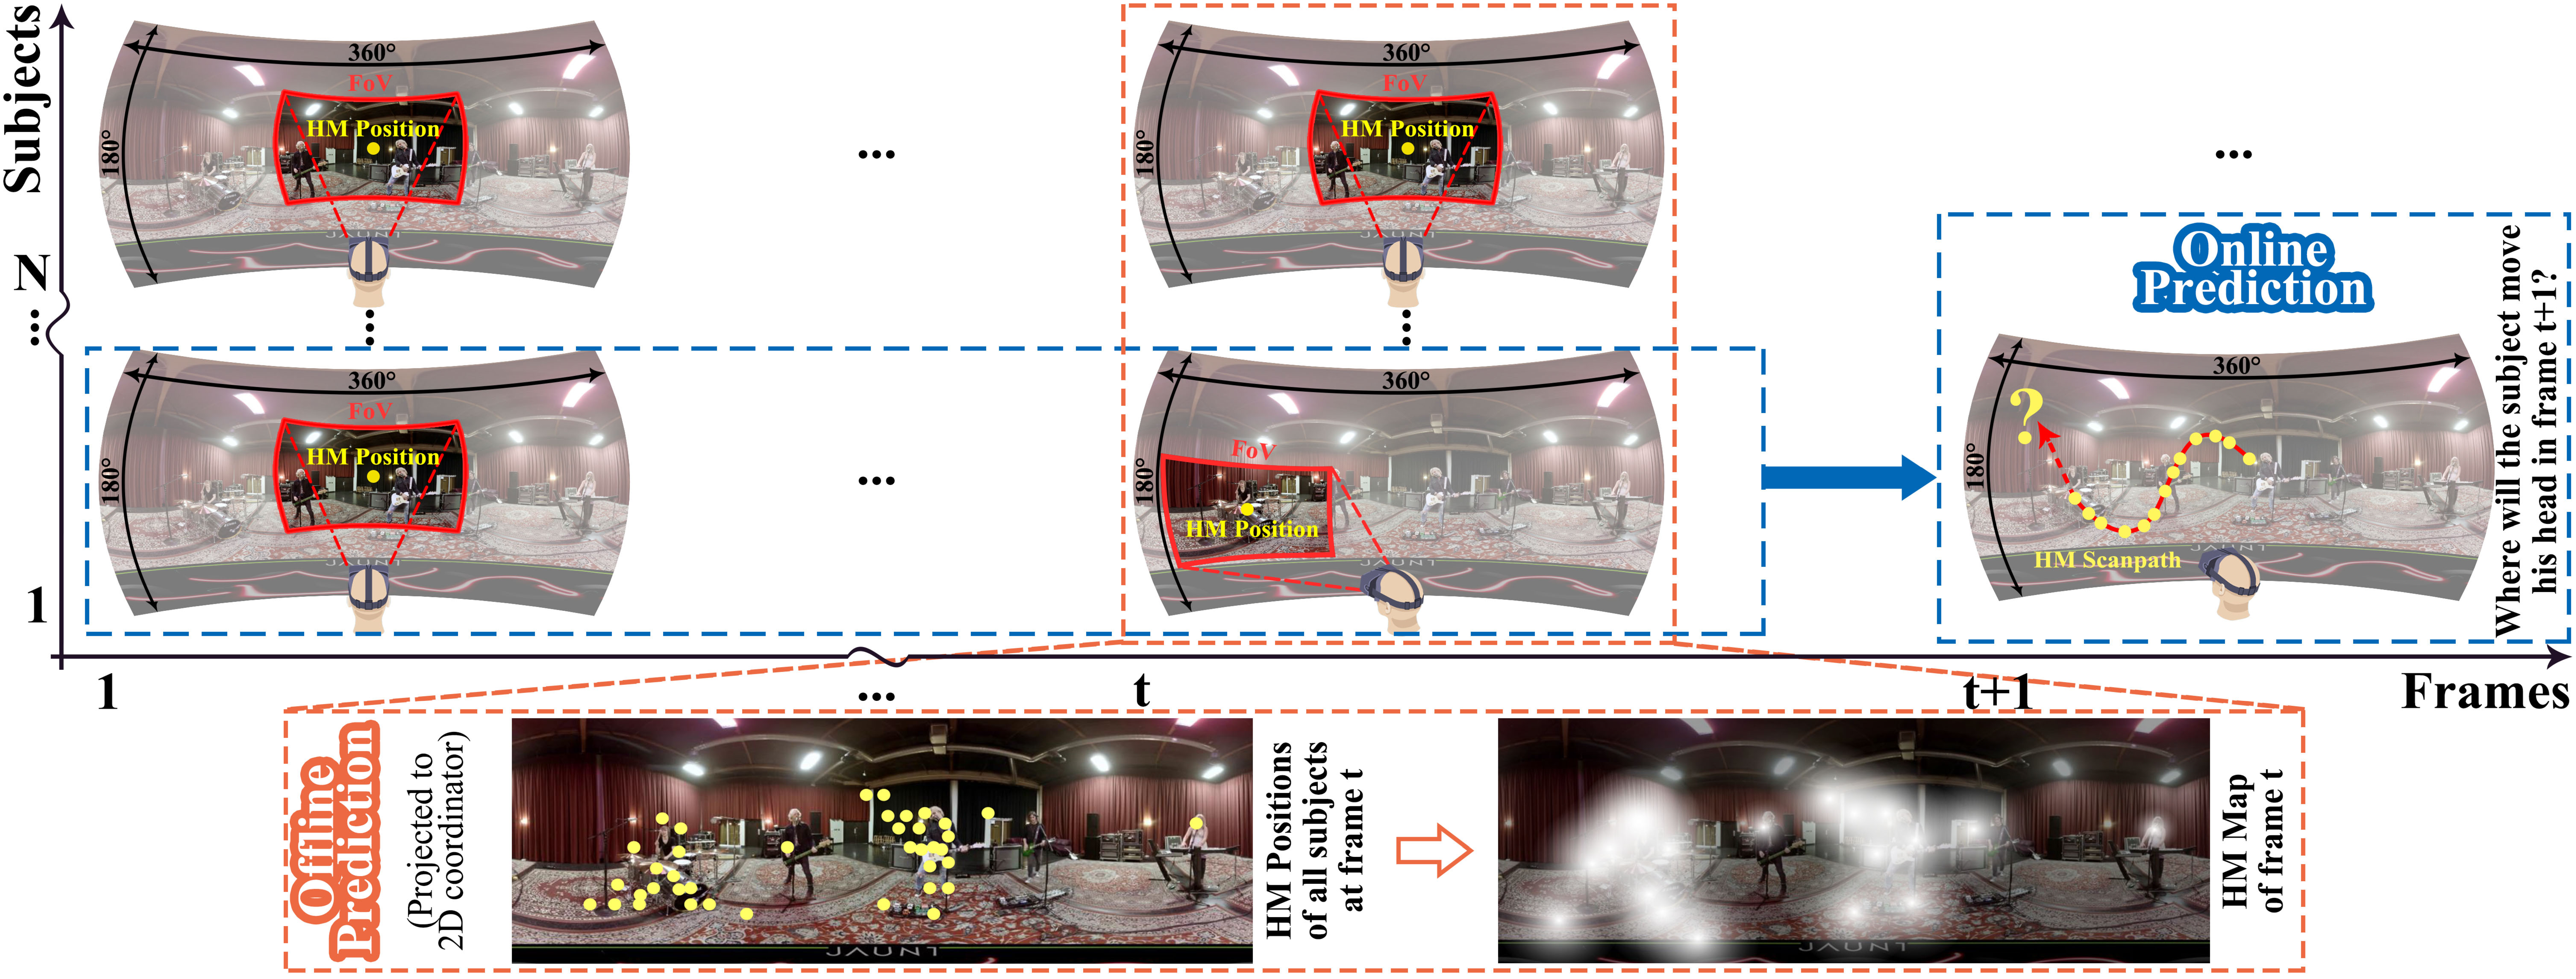
\includegraphics[width=1.6\columnwidth]{figures/introduction/fig_one}}
        \vspace{-.5em}
		\caption{\footnotesize{Illustration for FoVs and HM positions across different subjects. The heat map of HM positions from all subjects is also shown, which is defined as the HM map.}}
		\label{fig-one}
	\end{center}
\vspace{-2em}
\end{figure*}

To our best knowledge, there exists no offline work to predict the HM positions of multiple subjects in viewing panoramic video. The closest work is saliency detection on 2D video \cite{borji2013state}. The earliest approach for saliency detection was proposed by \textit{Itti et al.} \cite{itti1998model}, in which the features of color, intensity and orientation are combined to generate the saliency map of an image. Later, \textit{Itti et al.} \cite{itti2004automatic} proposed adding two features to \cite{itti1998model}, namely, motion and flicker contrast, for video saliency detection. Recently, several advanced approaches have been proposed for video saliency prediction. These advanced works include  the earth mover's distance (EMD) approach \cite{lin2013visual} and the Boolean map-based saliency model (BMS) \cite{zhang2016exploiting}.
Most recently, deep learning has been successfully applied in saliency detection,
such as SALICON \cite{huang2015salicon} and Liu's approach \cite{Liu2017cvpr}.
Saliency detection in 2D video assumes that humans are able to view all the content of each video frame.
However, this assumption does not hold for panoramic video, because subjects can only see a limited range of the FoV at a single sight, rather than the full panoramic range of $360^{\circ} \times 180^{\circ}$.
In fact, different regions of panoramic video are accessible to subjects via changing the positions of HM \cite{lowe2015visualization}.
In this paper, we find that different subjects are highly consistent in terms of HM positions.
This finding is based on establishing and analyzing a new database, which consists of the HM data of 58 subjects viewing 76 panoramic video sequences.
Then, we propose the offline-DHP approach to predict the consistent HM positions on panoramic video via generating the HM map for each single frame.
The HM maps are in the form of a sphere, and the positions in the HM maps are thus represented by the longitude and latitude in the geographic coordinate system (GDS) \cite{Goodchild2007}. This paper visualizes the spherical HM maps by projecting them onto the 2D plane.
Figure \ref{fig-one} demonstrates an example of the ground-truth HM map for a panoramic video frame. Similar to the saliency maps of 2D video, the HM maps of panoramic video are obtained by convoluting the HM positions with a 2D Gaussian filter\footnote{The two dimensions of the Gaussian filter are longitude and latitude, respectively.}.

%Then, we  propose a DRL based HM prediction (DHP) approach, which predicts the possible HM positions on panoramic video via generating the HM map for each single frame.
%Here, the HM maps of panoramic videos are similar to the saliency maps of 2D video.
%Figure \ref{fig-one} demonstrates an example of the ground-truth HM map for a panoramic video frame.
%As shown in this figure, HM positions of multiple subjects need to be predicted in an offline manner, such that the HM maps can be obtained.
%Therefore, our DHP approach is offline for yielding HM maps, namely off-line DHP.

Specifically, our offline-DHP approach yields the HM maps of panoramic video via predicting the HM scanpaths of multiple \textit{agents}, since subjects interactively control their HM positions along with some scanpaths according to video content.
First, we find from our database that the HM scanpaths of different subjects are highly consistent.
Meanwhile, subjects are normally initialized to view the center of the front region in the beginning frames of panoramic video.
Therefore, the HM positions at the subsequent frames can be yielded on the basis of the predicted scanpaths.
Additionally, we find from our database that the magnitudes and directions of HM scanpaths are with similarity across subjects.
In light of these findings, our offline-DHP approach models both the magnitudes and directions of HM scanpaths as the \textit{actions} of multiple DRL \textit{agents} and takes the viewed panoramic content as the \textit{observation} of the \textit{environment}.
As such, the DRL model can be learned to predict HM positions.
In training the DRL model, a \textit{reward} is designed to measure the difference of \textit{actions}  between the DRL \textit{agents} and subjects, indicating how well the \textit{agents} imitate humans in terms of HM scanpaths.
Then, the \textit{reward} is optimized to learn the parameters in the DRL model.
Given the learned model, the HM maps of panoramic video are generated upon the predicted HM positions, obtained from the scanpaths of several \textit{agents} in multiple DRL workflows.

%we propose a novel offline-DHP approach, as our offline approach for predicating HM positions on panoramic video.

For online HM prediction, the latest work of \cite{hu2017deep} proposed a deep 360 pilot, which automatically shifts viewing direction (equivalent to the HM position) when watching panoramic video. Specifically, the salient object is detected and tracked across panoramic video frames, via leveraging a region-based convolutional neural network (RCNN) \cite{ren2015faster} and recurrent neural network (RNN). Given the detected salient object and previous viewing directions, the deep 360 pilot predicts to transit HM position by learning a regressor. Since the deep 360 pilot relies heavily on one salient object, it is only suitable for some specific scenes that include one salient object, e.g., the sports scenes in \cite{hu2017deep}. It is still challenging to predict HM positions online for generic panoramic video, which may include more than one salient object (e.g., the panoramic video in Figure \ref{fig-one}). In this paper, we propose an online approach, namely online-DHP, to predict the HM positions on generic panoramic video. In contrast to \cite{hu2017deep}, our online-DHP approach does not need to detect the salient object using the RCNN. Rather, our online-DHP approach is based on attention-related content by leveraging the learned model of our offline-DHP approach. Then, a DRL algorithm is developed in our online-DHP approach to predict the HM positions in an online manner. Specifically, in the DRL algorithm, the \textit{agent} predicts the \textit{action} of the HM scanpath in the next frame, according to the ground-truth of the previous HM scanpath and \textit{observation} of video content. Consequently, the HM positions at the incoming frames can be predicted for our online-DHP approach.


This paper is the first attempt to apply the DRL algorithm in modeling human attention on panoramic video. The main contributions of this paper are three-fold:
\begin{itemize}
\item We establish a new panoramic video database that consists of HM positions of 58 subjects  across 76 panoramic video sequences, with a thorough analysis of their HM data.

\item We propose an offline-DHP approach to detect HM maps of panoramic video, and this approach predicts the consistent HM positions of multiple subjects.

\item We develop an online-DHP approach to predict the HM position of one subject at the next panoramic frame, based on video content and HM positions until the current frame.

\end{itemize}

%based on content of the current frame and knowledge of viewing directions in the previous frames.

%To our best knowledge, our work is a pioneering one in modeling attention on panoramic video using HM maps.




%To the best of our knowledge, there exists few work to model attention of subjects, especially their HMs, on panoramic video.
%The closest work is saliency detection on 2D video \cite{borji2013state}.
%Video saliency detection can be traced back to \cite{itti2004automatic}, in which \textit{ltti et al.} proposed to generate saliency maps of video frames, by linearly combining the conspicuity maps of feature channels on color, intensity, orientation, motion and flicker contrast.
%Later, some advanced approaches on saliency detection were proposed, such as \cite{itti2006bayesian, Hou2008dynamic, guo2010novel, lin2013visual, rudoy2013learning, hossein2015many, zhang2016exploiting, xu2017learning}.
%For example, Lin \textit{et al.} \cite{lin2013visual} applied earth mover's distance (EMD) to measure the center-surround difference in spatio-temporal receptive field, for yielding the dynamic saliency maps of videos.
%Hossein \textit{et al.} \cite{hossein2015many} proposed to predict video saliency upon bit allocation of each block in video coding.
%Most recently, deep learning \cite{bazzani2016recurrent, bak2016two, Liu2017cvpr} has been applied in video saliency detection.
%For example, Bazzani \textit{et al.} \cite{bazzani2016recurrent} proposed a recurrent mixture density model, which combines 3D convolutional neural network (CNN) and long short-term memory network (LSTM), for predicting video saliency.
%
%Saliency detection in 2D video assumes that humans are able to view all content of each video frame.
%This assumption does not hold for panoramic videos, as subjects can only see a limited range of FoV at a single sight, rather than the full panoramic range of $360^{\circ} \times 180^{\circ}$.
%In fact, different regions of panoramic video are accessible to subjects via changing the positions of HM \cite{lowe2015visualization}.
%For panoramic video of sport scenes, the most recent works \cite{lin2017tell, hu2017deep} proposed to predict the current HM position of one subject (called viewing angle in \cite{hu2017deep}) upon observed HM positions of this subject at previous frames.
%These works belong to online attention modeling of a single subject.
%Unfortunately, there is no offline approach to model attention of multiple subjects on panoramic video.
%In this paper, we establish a database consisting of 40 subjects' HM data on viewing 48 panoramic video sequences. Based on the established database, we argue that different subjects are consistent on HM positions, i.e., the longitude and latitude of their viewing directions in a panorama are similar.
%Hence, we propose an offline approach to predict HM positions of panoramic video via generating the HM map for each single frame, which is similar to saliency maps of 2D video.
%Figure 1 demonstrates an example of the ground-truth HM map for a panoramic video frame.
%To our best knowledge, our work is a pioneering one in modeling attention on panoramic video using HM maps.




\section{Related work}

\subsection{Saliency detection}
The only approach for predicting the HM positions of panoramic videos is the most recent work of \cite{su2016pano2vid}, in which Pano2Vid was proposed to obtain the FoV at each panoramic video frame. However, Pano2Vid primarily focuses on virtually generating a potential HM position at one frame, rather than modeling HM maps of multiple subjects at this frame. The closest work on predicting HM maps is saliency detection for 2D video, which is briefly reviewed in the following.

Saliency detection aims to predict the visual attention of humans on 2D videos, by generating saliency maps of video frames. The studies on visual saliency begin in 1998, when Itti and Koch \cite{itti1998model} found that the features of intensity, color and orientation in an image can be employed to detect its saliency map. Subsequently, they extended their work to video saliency detection \cite{itti2004automatic}, in which two dynamic features of motion and flicker contrast are combined with \cite{itti1998model} to detect saliency in 2D videos. Both \cite{itti1998model} and \cite{itti2004automatic} can be considered to be heuristic approaches for detecting saliency, since they utilize the understanding of the HVS to develop the computational models. Recently, some advanced heuristic approaches, e.g.,  \cite{itti2009bayesian, boccignone2008nonparametric, zhang2009sunday, guo2010novel, ren2013regularized, lin2013visual, zhang2016exploiting, hossein2015many, xu2017learning}, have been proposed to detect saliency in 2D videos. Specifically, \cite{itti2009bayesian} proposed a novel feature called \textit{surprise}, which measures how the visual change attracts human observers, based on the Kullback-Leibler (KL) divergence between spatio-temporal posterior and prior beliefs. Given the feature of \textit{surprise}, a Bayesian framework was developed in \cite{itti2009bayesian} for video saliency detection.  Some other Bayesian frameworks \cite{boccignone2008nonparametric, zhang2009sunday}  were also developed to detect video saliency. Besides, Lin \textit{et al.} \cite{lin2013visual} quantified the earth mover's distance (EMD) to measure the center-surround difference in spatio-temporal receptive field, generating saliency maps for 2D videos. Zhang \textit{et al.} \cite{zhang2016exploiting} explored the surround cue for saliency detection, by characterizing a set of binary images with random thresholds on color channels. Recently, \cite{hossein2015many} and \cite{xu2017learning} have investigated that some features (e.g., motion vector) in compressed domain are of high correlation with human attention, and these features are thus explored in video saliency detection.


Benefiting from the most recent success of deep learning, deep neural networks (DNNs) \cite{huang2015salicon, kruthiventi2015deepfix, wang2016RCNN, bazzani2016recurrent, Liu2017cvpr, bak2016two,wang2017deep} have also been  developed to detect 2D video saliency, rather than exploring the HVS-related features as in heuristic saliency detection approaches. These DNNs can be viewed as data-driven approaches. For static saliency detection, SALICON [19] fine-tuned the existing convolutional neural networks (CNNs), with a new saliency-related loss function. For dynamic saliency detection, \cite{bazzani2016recurrent} leveraged a deep convolutional 3D (C3D) network to learn the representations of human attention on 16 consecutive frames, and then a long short-term memory (LSTM) network connected with a mixture density network was learned to generate saliency maps using Gaussian mixture distribution. Similarly, Liu \textit{et al.} \cite{Liu2017cvpr} combined a CNN and multi-stream LSTM to detect saliency in videos with multiple faces. Moreover, other DNN structures have been developed to detect either static saliency \cite{kruthiventi2015deepfix, wang2016RCNN} or dynamic saliency \cite{bak2016two,bazzani2016recurrent,wang2017deep}.


\begin{figure}
\vspace{-1em}
	\begin{center}
		\centerline{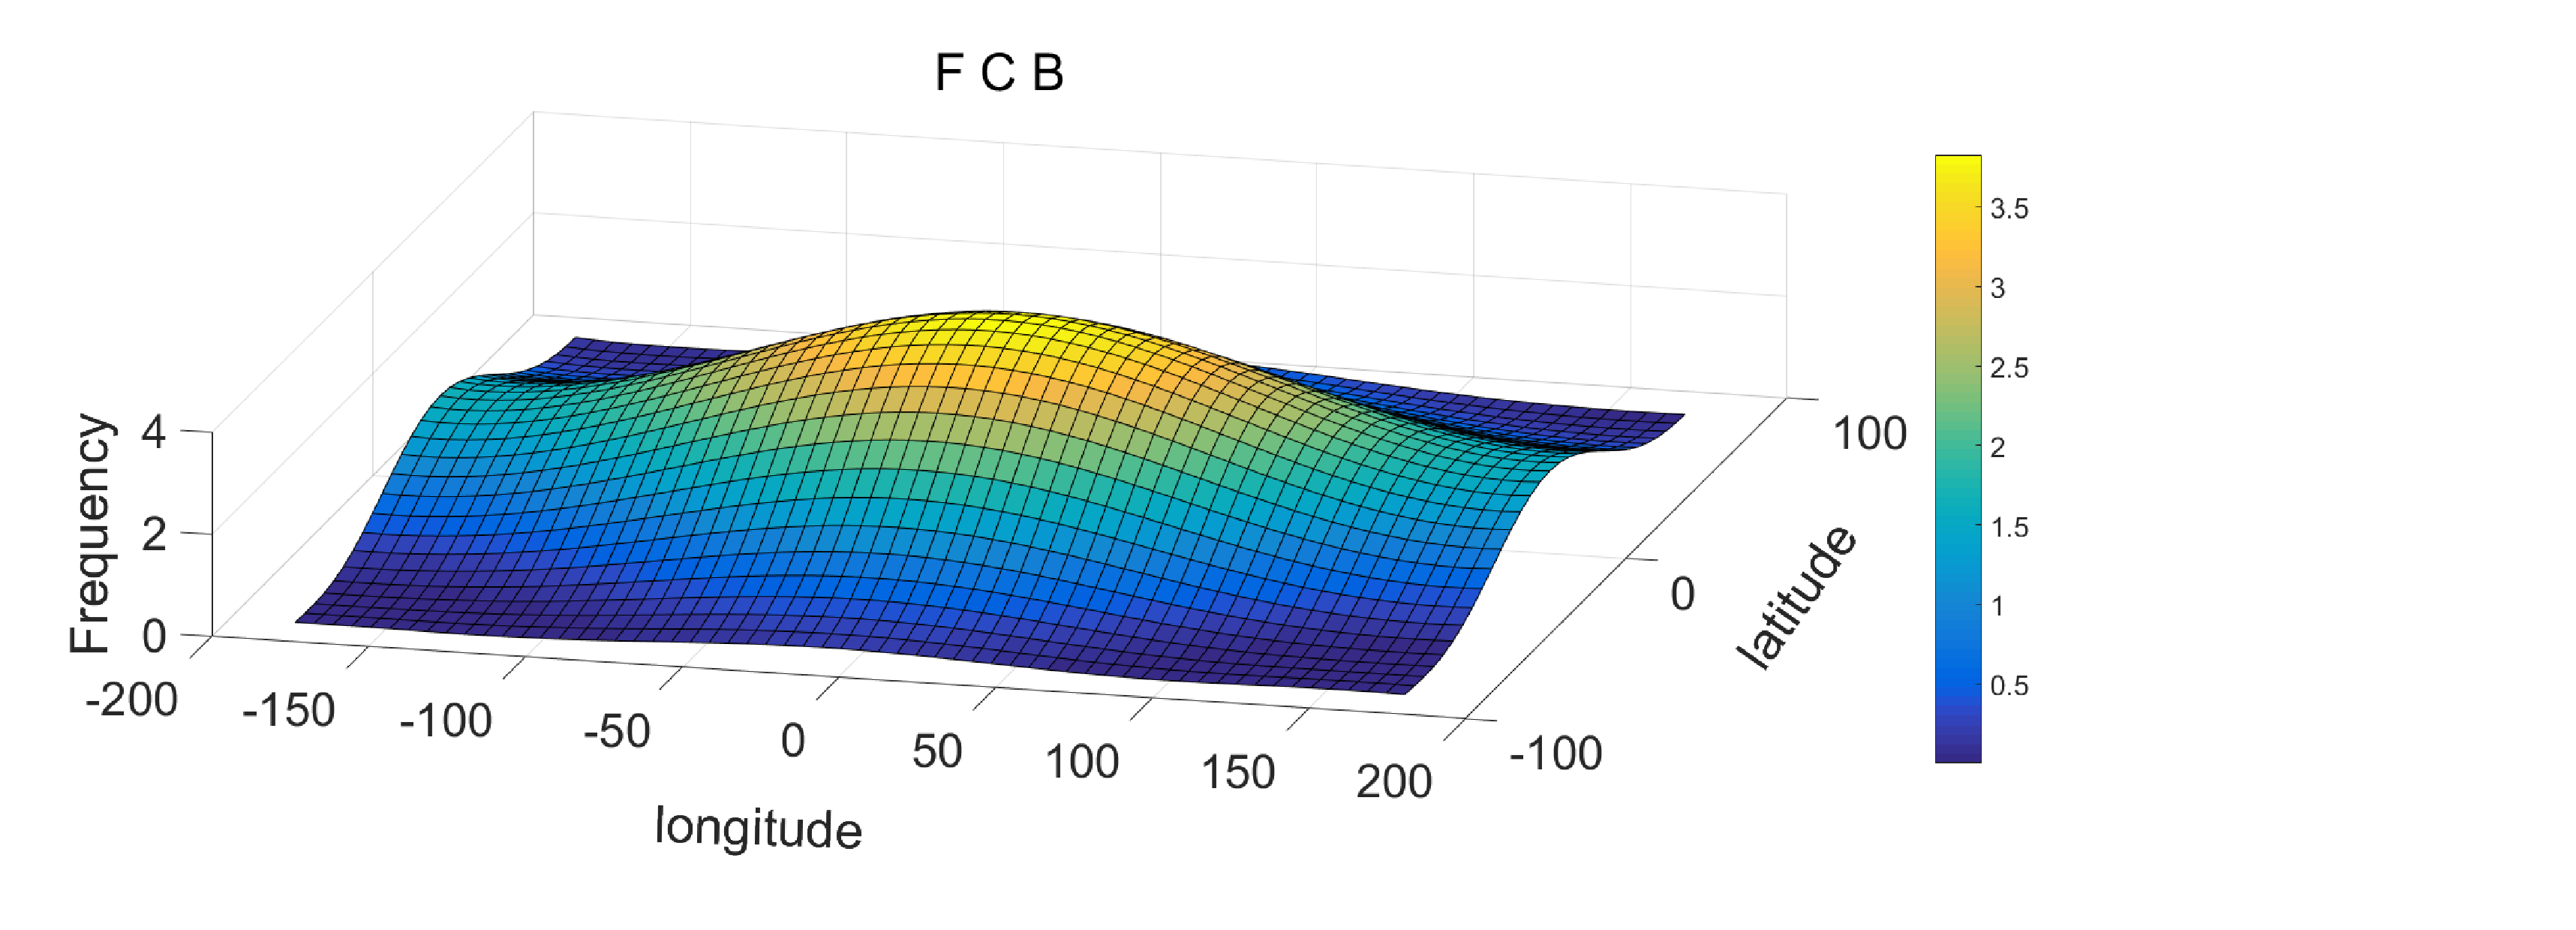
\includegraphics[width=.9\columnwidth]{figures/database/huoshantu}}%of
        \vspace{-.5em}
		\caption{\footnotesize{Distribution of 58 subjects' HM positions at different panoramic regions. It is calculated from all panoramic video frames of the PVS-HM database. }}
		\label{huoshantu}
	\end{center}
\vspace{-2.5em}
\end{figure}

Although saliency detection has been thoroughly studied in predicting eye movement on 2D videos, no works have been developed to predict HM positions on panoramic videos.
Similar to saliency detection for 2D videos, this paper proposes generating HM maps that represent the HM positions of multiple subjects. Hence, the HM maps model attention on panoramic videos. To obtain the HM maps of panoramic video, a DRL approach is developed for deciding the \textit{actions} of HM from multiple \textit{agents}. The \textit{actions} are decided based on the \textit{environment} of the panoramic video content, the features of which are automatically learned and then extracted by a DNN. Thus, our approach takes advantage of both deep learning and reinforcement learning, driven by the HM data of our panoramic video database.
Note that although few works apply DRL to predict human attention, the attention model is widely used in the opposite direction to improve the performance of reinforcement learning, e.g., \cite{minut2001reinforcement, mnih2014recurrent, jaderberg2016reinforcement, wang2016dueling}.


\begin{figure*}
\vspace{-1em}
	\begin{center}
		\centerline{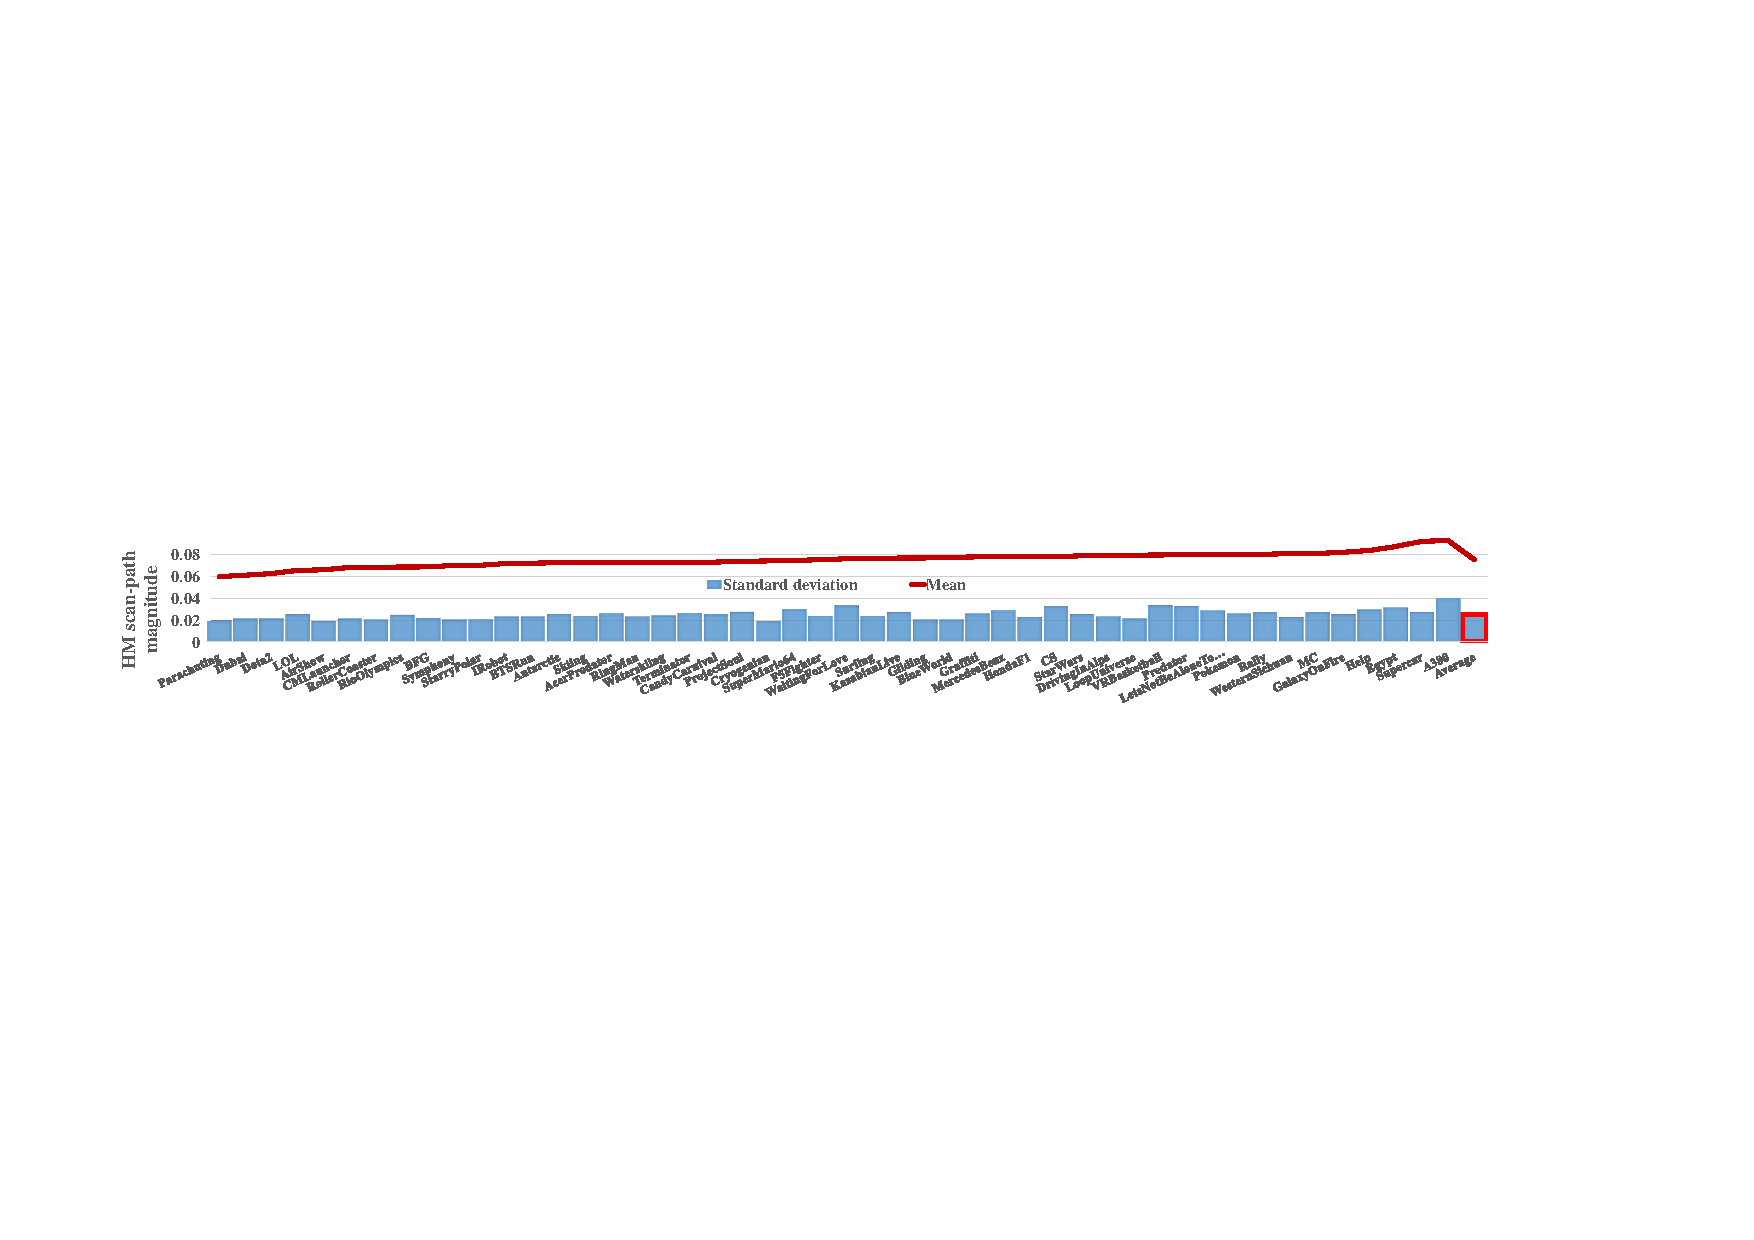
\includegraphics[width=2\columnwidth]{figures/database/consistence-magnitude}}
        \vspace{-1em}
		\caption{\footnotesize{Mean and standard deviation for the HM scanpath magnitude over different subjects, for the 76 panoramic video sequences in our PVS-HM database. The last column also shows the mean and standard deviation, averaged over all 76 sequences. }}
		\label{consistence-magnitude}
	\end{center}
\end{figure*}


\begin{figure*}
\vspace{-3em}
	\begin{center}
		\centerline{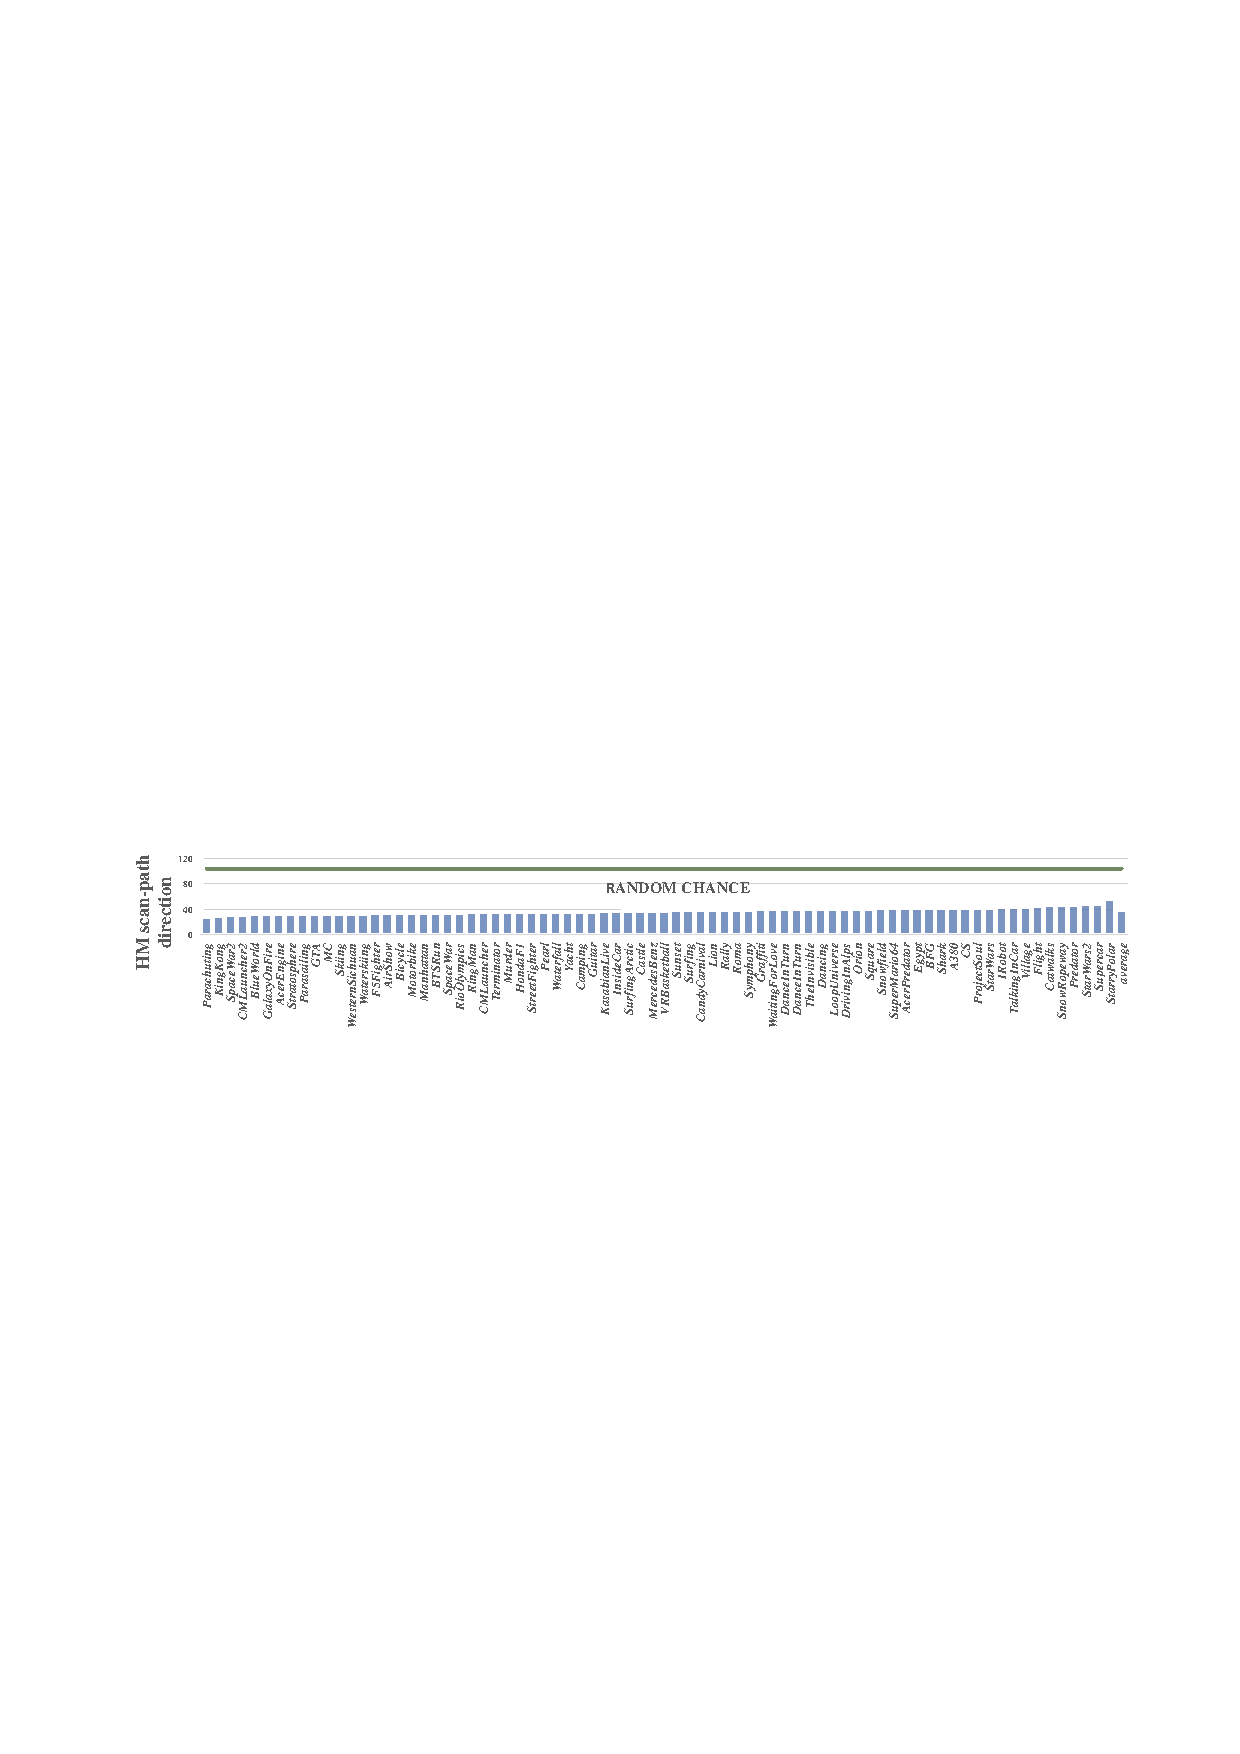
\includegraphics[width=2\columnwidth]{figures/database/direction-consistence}}%of
         \vspace{-1em}
		\caption{\footnotesize{Circular standard deviation for the HM scanpath directions, over the 76 panoramic video sequences in our PVS-HM database. The average results are also shown in the last column.}}
		\label{direction-consistence}
	\end{center}
\vspace{-2em}
\end{figure*}

\subsection{Virtual cinematography}
Virtual cinematography of panoramic video, which directs an imaginary camera to virtually capture natural FOV (NFOV), was proposed in \cite{foote2000flycam, sun2005region, su2016pano2vid, hu2017deep, lin2017tell}. In general, virtual cinematography attempts to agree with the HM positions of humans at each panoramic video frame. The early work of \cite{foote2000flycam} proposed cropping the object-of-interest in panoramic video, such that the NFOV can be generated for virtual cinematography. Later, in \cite{sun2005region}, the cropped object-of-interest is tracked across frames by a Kalman filter, for automatically controlling the virtual camera in virtual cinematography of panoramic video. The approach of \cite{sun2005region} can work on both compressed and uncompressed domains, because two methods were developed to detect the object-of-interest in compressed and uncompressed domains. The works of \cite{foote2000flycam, sun2005region} were both designed for the task of online virtual cinematography. These works can be considered as heuristic approaches, which are not trained or even evaluated on the ground-truth HM data of human subjects.

Most recently, data-driven approaches have boosted the development of virtual cinematography for panoramic videos. Specifically, Pano2Vid \cite{su2016pano2vid} learns to generate NFOV at each panoramic frame. However, the learning mechanism of Pano2Vid is offline. In fact, NFOV can be estimated at each frame in an online manner, which uses the observed HM positions of the previous frames to correct the estimation of NFOV at the current frame. To this end, online virtual cinematography \cite{hu2017deep, lin2017tell} has been studied in a data-driven way.
Specifically, a state-of-the-art virtual cinematography  approach, the deep 360 pilot,  was proposed in \cite{hu2017deep}, which is a deep-learning-based \textit{agent} that smoothly tracks the object-of-interest for panoramic video. In other words, the \textit{agent} transits the HM position across video frames to track the key object detected by the RCNN, given the observed HM positions at previous frames. Consequently, NFOV can be generated online for automatically displaying the object-of-interest in virtual cinematography of panoramic videos. In fact, object-of-interest tracking in panoramic video refers to continuously focusing and refocusing the intended targets. Both focusing and refocusing require a subject to catch up the object. Such a task is challenging in extreme-sports videos, as the object-of-interest may be moving fast. Therefore, Lin \textit{et al.} \cite{lin2017tell} investigated two focus assistance techniques to help the subject track the key object in viewing panoramic video, in which the potential HM position attended to the object-of-interest needs to be determined and provided for the subject.

The above approaches of \cite{foote2000flycam, sun2005region, su2016pano2vid, hu2017deep, lin2017tell}  all depend on the detector of the object-of-interest. Thus, they can only be applied in some specific panoramic videos with salient objects, such as video conferencing or classroom scenes in \cite{foote2000flycam, sun2005region} and the sports videos in \cite{su2016pano2vid, hu2017deep, lin2017tell}. Different from these conventional approaches, our online-DHP approach is based on the learned model of our offline approach, which encodes HM-related content rather than detecting the object-of-interest. Consequently, our approach is object free and thus more suitable for generic panoramic videos.

%Both the works of \cite{lin2017tell, hu2017deep} are designed for the task of virtual cinematography, which directs an imaginary camera to virtually capture NFOV from panoramic videos. Also, the work of \cite{su2016pano2vid} also targets at virtual cinematography of panoramic video, but in an offline manner. In fact, most of existing virtual cinematography works \cite{} concentrate on camera manipulation within a simple virtual environment, rather than panoramic scenes.





%The initial work of online HM prediction can be traced back to automatic cinematography of panoramic video \cite{}.





\section{Database establishment and analysis}
\label{Database_establishment_and_analysis}

\subsection{Database establishment}
\label{Database_establishment}

In this section, we collect a new database that includes 76 panoramic video sequences with the HM data of 58 subjects, called the PVS-HM database. Our PVS-HM database allows quantitative analysis of subjects' HM on panoramic video, and it can also be used for learning to predict where humans look at panoramic video. Our database is available at  \url{https://github.com/YuhangSong/dhp} for facilitating future research. In the following, we present how we conducted the experiment to obtain the PVS-HM database.

First, we selected 76 panoramic video sequences from YouTube and VRCun, with resolutions ranging from 3K to 8K.
As shown in Table \ref{tab:CC}, the content of these sequences is diverse, including computer animation (CA), driving, action sports, movies, video games, scenery, and so forth.
Then, the duration of each sequence was cut to be from 10 to 80 seconds (averagely 26.9 seconds), such that fatigue can be reduced when viewing panoramic video.
To ensure video quality, all panoramic video sequences were compressed using H.265 \cite{Sullivan2013Overview} without any change in bit-rates.
Note that the audio tracks were removed to avoid the impact of acoustic information on visual attention.

In our experiment, 58 subjects (41 males and 17 females, ranging in age from 18 to 36) wore the HMD of an HTC Vive to view all 76 panoramic video sequences at a random display order.
When watching panoramic video, the subjects were seated on a swivel chair and were allowed to turn around freely, such that all panoramic regions are accessible.
To avoid eye fatigue and motion sickness, the subjects had a 5 minute rest after viewing each session of 19 sequences.
With the support of the software development kit (SDK) of HTC Vive, we recorded the posture data of each subject as they viewed the panoramic video sequences.
Based on the recorded posture data, the HM data of all 58 subjects at each frame of the panoramic video sequences were obtained and stored for our PVS-HM database, in terms of longitude and latitude in the GDS.


\subsection{Database analysis}
\label{Database_analysis}

In this section, we mine our PVS-HM database to analyze HM data of different subjects across panoramic video sequences.
Specifically, we have the following six findings.

%\begin{table*}
%\begin{center}
%  \caption{CC between ground-truth HM maps of Groups $A$ and $B$, for each panoramic video sequence} \label{tab:CC}
%  \tiny
%  \resizebox{\textwidth}{!}{
%  \begin{tabular}{*{4}{|c|c|c}|}
%  \hline
%  \tabincell{c}{Cate-\\gory} & Name & CC & \tabincell{c}{Cate-\\gory} & Name & CC & \tabincell{c}{Cate-\\gory} & Name & CC & \tabincell{c}{Cate-\\gory} & Name & CC \\
%  \hline
%  \multirow{6}{*}{\rotatebox{90}{CA}} & AcerPredator & 0.839$\pm$0.087
%&
%  \multirow{6}{*}{\rotatebox{90}{Driving}} & AirShow & 0.783$\pm$0.078
% &
%  \multirow{6}{*}{\rotatebox{90}{Others}} & A380 & 0.839$\pm$0.106
% &
%  \multirow{6}{*}{\rotatebox{90}{Video Game}} & CS & 0.819$\pm$0.084
% \\
%  \cline{2-3} \cline{5-6} \cline{8-9} \cline{11-12}
%  & BFG & 0.644$\pm$0.146
% & & DrivingInAlps & 0.857$\pm$0.071
% & & CandyCarnival & 0.723$\pm$0.094
% & & Dota2 & 0.714$\pm$0.103
% \\
%  \cline{2-3} \cline{5-6} \cline{8-9} \cline{11-12}
%  & CMLauncher & 0.828$\pm$0.119
% & & F5Fighter & 0.592$\pm$0.126
% & & MercedesBenz & 0.592$\pm$0.133
% & & GalaxyOnFire & 0.762$\pm$0.084
% \\
%  \cline{2-3} \cline{5-6} \cline{8-9} \cline{11-12}
%  & Cryogenian & 0.526$\pm$0.174
% & & HondaF1 & 0.872$\pm$0.053
% & & RingMan & 0.897$\pm$0.054
% & & LOL & 0.724$\pm$0.097
% \\
%  \cline{2-3} \cline{5-6} \cline{8-9} \cline{11-12}
%  & LoopUniverse & 0.779$\pm$0.078
% & & Rally & 0.867$\pm$0.047
% & & RioOlympics & 0.624$\pm$0.123
% & & MC & 0.726$\pm$0.115
% \\
%  \cline{2-3} \cline{5-6} \cline{8-9} \cline{11-12}
%  & Pokemon & 0.607$\pm$0.182
% & & Supercar & 0.854$\pm$0.064
% & & VRBasketball & 0.770$\pm$0.105
% & & SuperMario64 & 0.860$\pm$0.054
% \\
%  \hline
%  \multirow{6}{*}{\rotatebox{90}{Movie}} & Help & 0.859$\pm$0.122
% &
%  \multirow{6}{*}{\rotatebox{90}{Scenery}} & Antarctic & 0.674$\pm$0.135
% &
%  \multirow{6}{*}{\rotatebox{90}{Show}} & BTSRun & 0.867$\pm$0.061
% &
%  \multirow{6}{*}{\rotatebox{90}{Action Sports}} & Gliding & 0.528$\pm$0.158
% \\
%  \cline{2-3} \cline{5-6} \cline{8-9} \cline{11-12}
%  & IRobot & 0.771$\pm$0.078
% & & BlueWorld & 0.559$\pm$0.156
% & & Graffiti & 0.807$\pm$0.100
% & & Parachuting & 0.628$\pm$0.157
% \\
%  \cline{2-3} \cline{5-6} \cline{8-9} \cline{11-12}
%  & Predator & 0.696$\pm$0.124
% & & Dubai & 0.646$\pm$0.133
% & & KasabianLive & 0.722$\pm$0.132
% & & RollerCoaster & 0.834$\pm$0.078
% \\
%  \cline{2-3} \cline{5-6} \cline{8-9} \cline{11-12}
%  & ProjectSoul & 0.918$\pm$0.053
% & & Egypt & 0.665$\pm$0.131
% & & NotBeAloneTonight & 0.587$\pm$0.131
% & & Skiing & 0.766$\pm$0.104
% \\
%  \cline{2-3} \cline{5-6} \cline{8-9} \cline{11-12}
%  & StarWars & 0.950$\pm$0.016
% & & StarryPolar & 0.495$\pm$0.152
% & & Symphony & 0.779$\pm$0.096
% & & Surfing & 0.830$\pm$0.096
% \\
%  \cline{2-3} \cline{5-6} \cline{8-9} \cline{11-12}
%  & Terminator & 0.843$\pm$0.078
% & & WesternSichuan & 0.667$\pm$0.138
% & & VRBasketball & 0.770$\pm$0.105
% & & Waterskiing & 0.781$\pm$0.128
% \\
%  \hline
%  \multicolumn{2}{|c|}{Overall} & \multicolumn{10}{c|}{0.745$\pm$ 0.114}\\
%  \hline
%  \end{tabular}}
%\end{center}
%\end{table*}

%TABLE HA_HB_NEW
\begin{table*}
\begin{center}
  \caption{CC values between the ground-truth HM maps of Groups $A$ and $B$, for each panoramic video sequence.} \label{tab:CC}
  \vspace{-1em}
  \tiny
  \resizebox{\textwidth}{!}{
  \begin{tabular}{*{4}{|c|c|c}|}
  \hline
  \tabincell{c}{Cate-\\gory} & Name & CC & \tabincell{c}{Cate-\\gory} & Name & CC & \tabincell{c}{Cate-\\gory} & Name & CC & \tabincell{c}{Cate-\\gory} & Name & CC \\
  \hline
  \multirow{10}{*}{\rotatebox{90}{CA}} & AcerEngine & 0.891$\pm$0.058
&
  \multirow{10}{*}{\rotatebox{90}{Others}} & A380 & 0.867$\pm$0.058
 &
  \multirow{10}{*}{\rotatebox{90}{Driving}} & AirShow & 0.883$\pm$0.033
 &
  \multirow{10}{*}{\rotatebox{90}{Show}} & BTSRun & 0.926$\pm$0.041
\\
\cline{2-3} \cline{5-6} \cline{8-9} \cline{11-12}

 & AcerPredator & 0.876$\pm$0.063

& & Camping & 0.851$\pm$0.073

& & Bicycle & 0.953$\pm$0.021

& & Catwalks & 0.834$\pm$0.069

\\
\cline{2-3} \cline{5-6} \cline{8-9} \cline{11-12}

 & BFG & 0.732$\pm$0.101

& & CandyCarnival & 0.830$\pm$0.088

& & DrivingInAlps & 0.858$\pm$0.073

& & DanceInTurn & 0.934$\pm$0.030

\\
\cline{2-3} \cline{5-6} \cline{8-9} \cline{11-12}

 & CMLauncher & 0.894$\pm$0.041

& & Lion & 0.937$\pm$0.034

& & F5Fighter & 0.572$\pm$0.109

& & Dancing & 0.906$\pm$0.052

\\
\cline{2-3} \cline{5-6} \cline{8-9} \cline{11-12}

 & CMLauncher2 & 0.924$\pm$0.045

& & MercedesBenz & 0.685$\pm$0.137

& & HondaF1 & 0.944$\pm$0.020

& & Graffiti & 0.906$\pm$0.037

\\
\cline{2-3} \cline{5-6} \cline{8-9} \cline{11-12}

 & LoopUniverse & 0.881$\pm$0.044

& & RingMan & 0.923$\pm$0.032

& & InsideCar & 0.903$\pm$0.036

& & Guitar & 0.866$\pm$0.096

\\
\cline{2-3} \cline{5-6} \cline{8-9} \cline{11-12}

 & Orion & 0.810$\pm$0.082

& & Shark & 0.812$\pm$0.116

& & Rally & 0.925$\pm$0.025

& & KasabianLive & 0.819$\pm$0.087

\\
\cline{2-3} \cline{5-6} \cline{8-9} \cline{11-12}

 & Pearl & 0.838$\pm$0.120

& & Square & 0.842$\pm$0.076

& & Stratosphere & 0.792$\pm$0.090

& & NotBeAloneTonight & 0.695$\pm$0.104

\\
\cline{2-3} \cline{5-6} \cline{8-9} \cline{11-12}

 & Roma & 0.896$\pm$0.054

& & TalkingInCar & 0.858$\pm$0.078

& & VRBasketball & 0.739$\pm$0.098

& & Symphony & 0.826$\pm$0.068
 \\
  \hline
 \multirow{10}{*}{\rotatebox{90}{VideoGame}} & Yacht & 0.780$\pm$0.126
&
 \multirow{10}{*}{\rotatebox{90}{Movie}} & IRobot & 0.907$\pm$0.029
&
 \multirow{10}{*}{\rotatebox{90}{Scenery}} & BlueWorld & 0.793$\pm$0.159
&
 \multirow{10}{*}{\rotatebox{90}{ActionSports}} & Supercar & 0.915$\pm$0.041
\\
\cline{2-3} \cline{5-6} \cline{8-9} \cline{11-12}

 & WaitingForLove & 0.867$\pm$0.083

& & KingKong & 0.740$\pm$0.091

& & Castle & 0.698$\pm$0.105

& & Flight & 0.834$\pm$0.072

\\
\cline{2-3} \cline{5-6} \cline{8-9} \cline{11-12}

 & CS & 0.872$\pm$0.061

& & Murder & 0.921$\pm$0.058

& & Egypt & 0.779$\pm$0.094

& & Motorbike & 0.746$\pm$0.105

\\
\cline{2-3} \cline{5-6} \cline{8-9} \cline{11-12}

 & GalaxyOnFire & 0.895$\pm$0.062

& & Predator & 0.743$\pm$0.132

& & Manhattan & 0.795$\pm$0.085

& & Parachuting & 0.777$\pm$0.103

\\
\cline{2-3} \cline{5-6} \cline{8-9} \cline{11-12}

 & GTA & 0.930$\pm$0.026

& & ProjectSoul & 0.946$\pm$0.024

& & Snowfield & 0.824$\pm$0.142

& & Parasailing & 0.836$\pm$0.058

\\
\cline{2-3} \cline{5-6} \cline{8-9} \cline{11-12}

 & MC & 0.728$\pm$0.124

& & StarWars & 0.910$\pm$0.038

& & StarryPolar & 0.637$\pm$0.120

& & Skiing & 0.748$\pm$0.099

\\
\cline{2-3} \cline{5-6} \cline{8-9} \cline{11-12}

 & SpaceWar & 0.681$\pm$0.116

& & StarWars2 & 0.912$\pm$0.035

& & Sunset & 0.746$\pm$0.080

& & SnowRopeway & 0.728$\pm$0.093

\\
\cline{2-3} \cline{5-6} \cline{8-9} \cline{11-12}

 & SpaceWar2 & 0.577$\pm$0.148

& & Terminator & 0.908$\pm$0.054

& & Village & 0.819$\pm$0.084

& & Surfing & 0.850$\pm$0.080

\\
\cline{2-3} \cline{5-6} \cline{8-9} \cline{11-12}

 & StreetFighter & 0.930$\pm$0.023

& & TheInvisible & 0.871$\pm$0.052

& & Waterfall & 0.824$\pm$0.066

& & SurfingArctic & 0.695$\pm$0.119
 \\
  \hline
  \multicolumn{1}{|c}{Overall} & \multicolumn{2}{c|}{0.830$\pm$ 0.075} & \multicolumn{1}{c|}{Gaussian distribution} & \multicolumn{2}{c|}{$5\times 10^{-5}$$\pm$ 0.004} & \multicolumn{1}{c|}{Uniform distribution} & \multicolumn{2}{c|}{$4\times 10^{-4}$$\pm$ 0.003}
  & \multicolumn{1}{c|}{FCB} & \multicolumn{2}{c|}{0.514$\pm$ 0.184}\\
  \hline
  \end{tabular}}
\end{center}
\end{table*}



\begin{figure*}
\vspace{-1.5em}
	\begin{center}
		\centerline{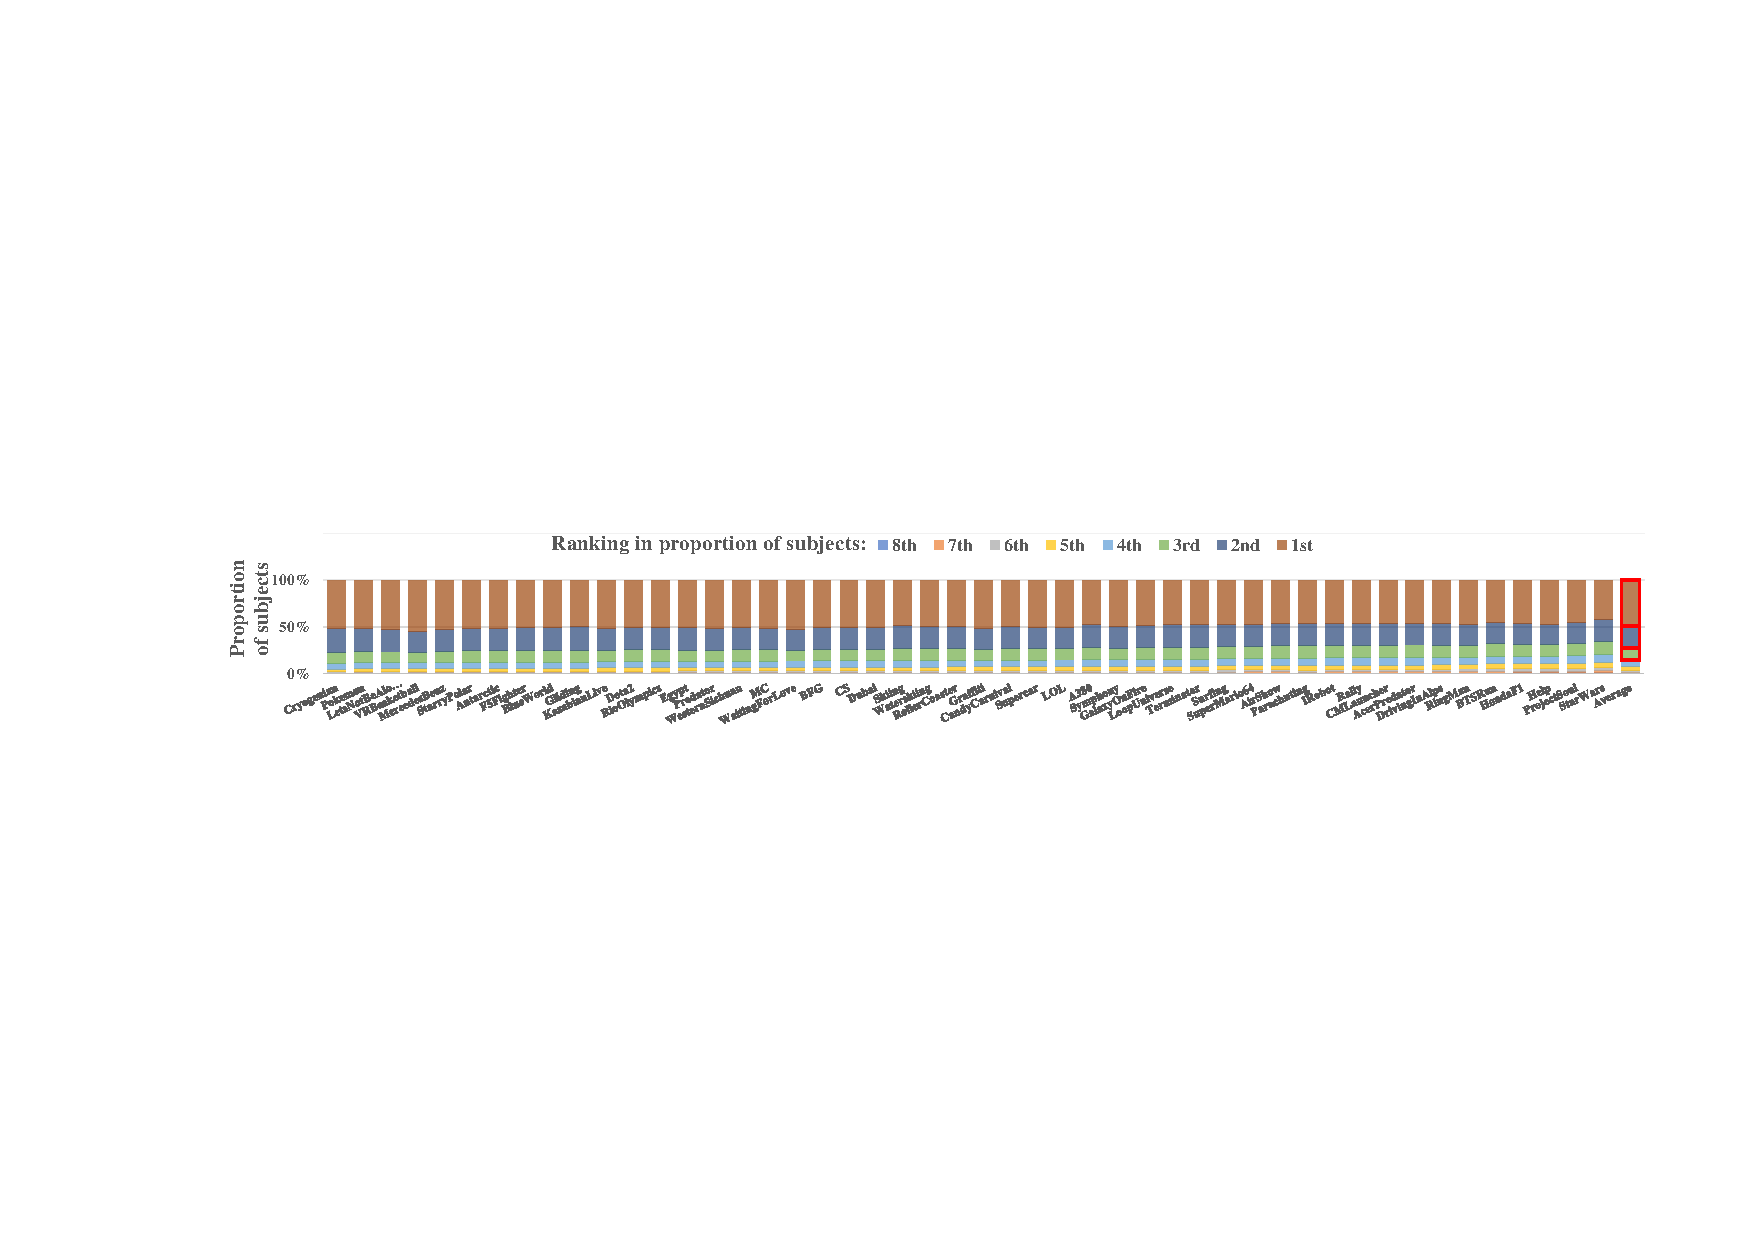
\includegraphics[width=2\columnwidth]{figures/database/direction-consistence-distribution}}%of
        \vspace{-1.5em}
		\caption{\footnotesize{Distribution of the HM scanpaths over 8 discrete directions, for the 76 sequences from our PVS-HM database. Note that the proportions of subjects, whose HM scanpath directions fall into each discrete direction, are ranked in the descending order and are then shown in this figure.}}
		\label{direction-consistence-distribution}
	\end{center}
\vspace{-2em}
\end{figure*}

\emph{Finding 1:  The HM positions on panoramic video possess front center bias (FCB). }
\\ \textit{Analysis:} We investigate whether FCB exists when people view panoramic video. This investigation is performed by calculating the numbers of HM positions in different regions of video frames. First, the $360^{\circ} \times 180^{\circ}$ panoramic region of each frame is equally segmented to be $60^{\circ} \times 30^{\circ}$ grids. Then, the numbers of HM positions of 58 subjects are counted for each segmented grid. Consequently, the frequency of HM positions in different panoramic regions is obtained, and it is shown in Figure \ref{huoshantu}. Note that the frequency results presented in Figure \ref{huoshantu} are obtained by averaging over all panoramic video frames of the PVS-HM database. We can see from this figure that the HM positions of 58 subjects are more likely to be attracted by the front center regions. This completes the analysis of Finding 1.

\emph{Finding 2: When watching panoramic video, different subjects are highly consistent in HM positions.}
\\ \textit{Analysis:} In our PVS-HM database, we randomly divide all 58 subjects into two equal-size groups, $A$ and $B$.
For each frame of 76 sequences, the ground-truth HM maps of Groups $A$ and $B$ are generated by convolving with a 2D Gaussian filter over the collected HM data, along with longitude and latitude.
They are denoted as $\mathbf{H}_A$ and $\mathbf{H}_B$, respectively.
For a panoramic frame, we quantify the correlation between $\mathbf{H}_A$ and $\mathbf{H}_B$ using linear correlation coefficient (CC) \cite{li2015data}.
Table~\ref{tab:CC} lists the average CC ($\pm$ standard deviations) between $\mathbf{H}_A$ and $\mathbf{H}_B$ over all frames, for each sequence.
We further show in  Table~\ref{tab:CC} the CC values between $\mathbf{H}_A$ and the maps generated by Gaussian distribution, uniform distribution and FCB.
It can be seen from this table that the CC values of Groups $A$ and $B$ are rather high, and that the average CC result of the two groups is significantly higher than those of a Gaussian distribution, uniform distribution and FCB.
Thus, it is clear that the HM positions of different subjects are highly consistent.
This completes the analysis of \textit{Finding 2}.







\emph{Finding 3: The magnitude of HM scanpaths is similar across subjects, when viewing the same panoramic video.}
\\ \textit{Analysis:} The HM scanpaths can be decomposed into magnitude and direction.
 Here, we measure the magnitude of HM scanpaths across different subjects.
For each individual sequence in our PVS-HM database, Figure \ref{consistence-magnitude} plots the mean and standard deviation of HM scanpath magnitude over all 58 subjects.
The last column of Figure \ref{consistence-magnitude} also shows the mean and standard deviation of HM scanpath magnitudes, averaged over all 76 sequences.
As shown in this figure, the standard deviation is considerably less than the mean value, for all 76 sequences and for the overall results.
Thus, we can conclude that similarity exists for the magnitude of HM scanpaths across subjects, when the subjects watch the same panoramic sequence.
This completes the analysis of \textit{Finding 3}.

 %rom this figure, we can see that the standard deviation of $22.7$ degree per second is far less than the mean of $47.7$ degree per second, for scanpath magnitudes of HM from different subjects.

\begin{figure}
\vspace{-1.5em}
	\begin{center}
		\centerline{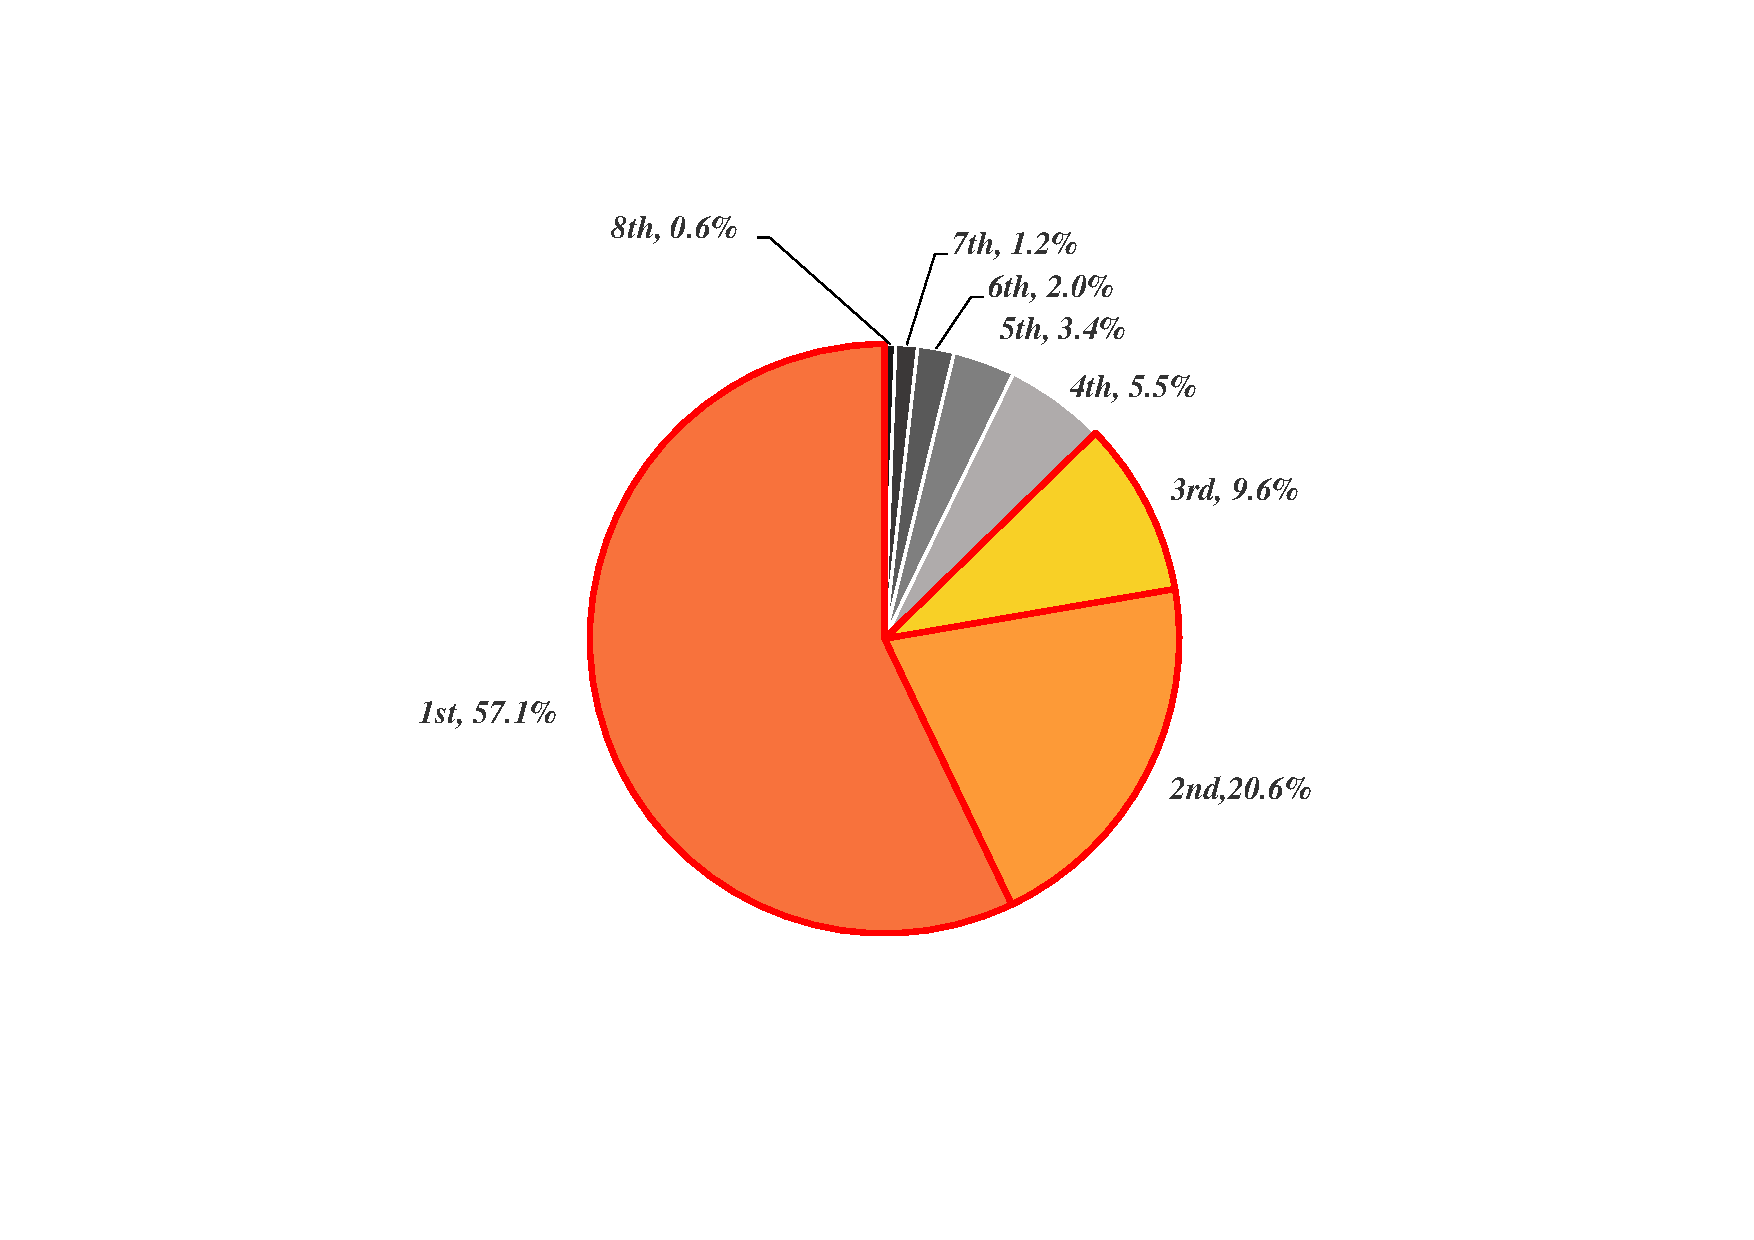
\includegraphics[width=.6\columnwidth]{figures/database/direction-consistence-distribution-pie}}%of
\vspace{-1em}
		\caption{\footnotesize{Proportions of subjects with HM scanpaths falling into each of 8 ranked directions. The proportions are averaged over all 76 sequences in the PVS-HM database. }}
		\label{direction-consistence-pie}
	\end{center}
\vspace{-3.5em}
\end{figure}


\emph{Finding 4: The direction of HM scanpaths on panoramic video is highly consistent across subjects.}
\\ \textit{Analysis:} In  our PVS-HM database, we evaluate the consistency of the HM scanpath direction among all 58 subjects.
Specifically, we evaluate the direction of the scanpath starting from the consistent HM regions, since \textit{Finding 2} has shown that the HM positions of different subjects are highly consistent. In our PVS-HM database, the consistent regions are extracted from 76 panoramic video sequences, which have the HM positions of at least 12 subjects within a small \textit{great-circle distance} range of $3^{\circ}$ \cite{matin1974saccadic}. For each panoramic video sequence, Figure \ref{direction-consistence} shows the circular standard deviation \cite{frederic2010mean} of HM scanpath directions, starting from the consistent HM regions within one-second time slot\footnote{We conducted our experiments with time slot being $0.1$, $1$ and $2$ seconds, and the results are similar.}. The last column of Figure \ref{direction-consistence} also reports the circular standard deviation averaged over all 76 sequences.
We can see from this figure that the circular standard deviation of the HM scanpath direction is $38.1^{\circ}$ on average, and it is significantly less than the value of $103.9^{\circ}$ of randomly generated HM scanpath directions. Moreover, the HM scanpath directions of all 76 sequences have considerably smaller circular standard deviations, compared to the random scanpaths.
This implies that high consistency exists on directions of HM scanpaths across subjects.
Consequently, \textit{Finding 4} is validated.

\begin{figure}
	\begin{center}
     \vspace{-1em}
		\centerline{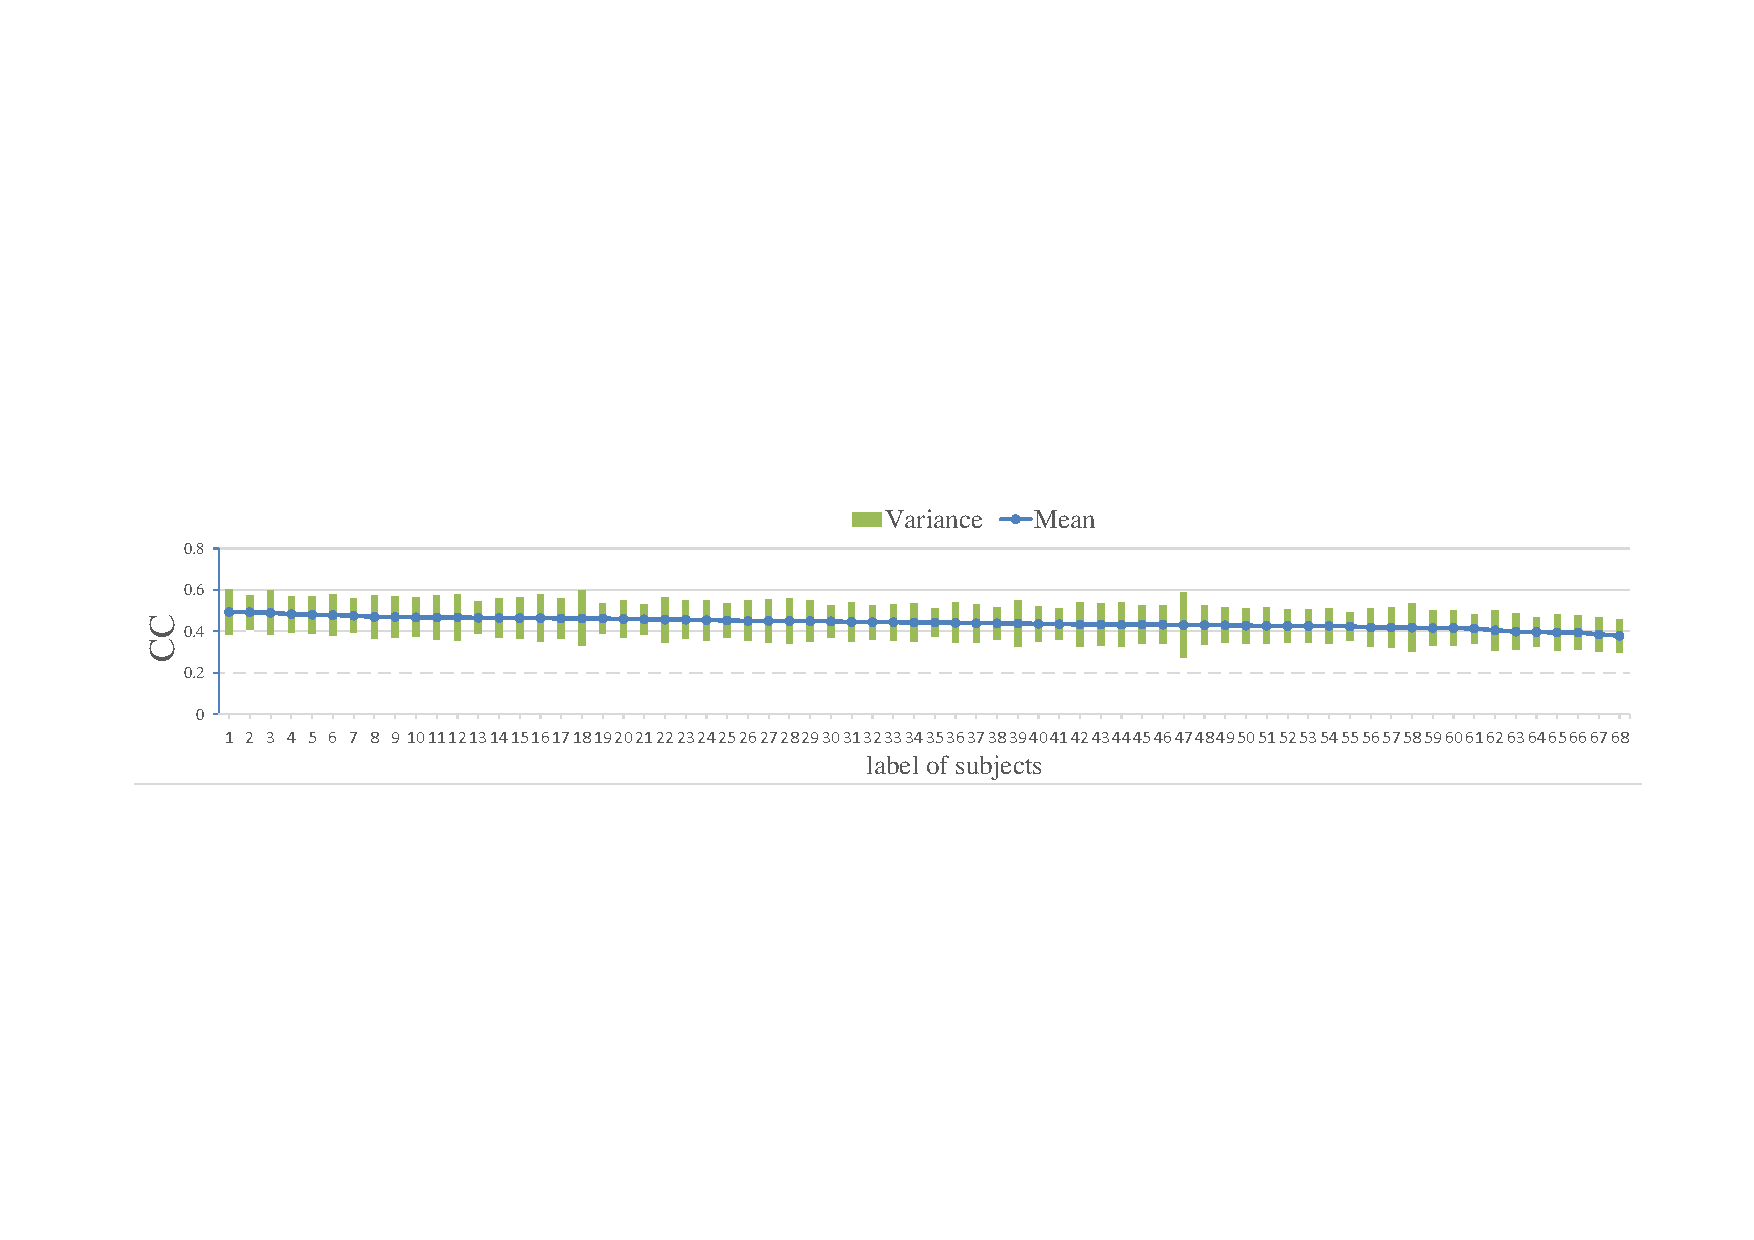
\includegraphics[width=.95\columnwidth]{figures/database/consi_on_time}}%of
        \vspace{-1em}
		\caption{\footnotesize{CC values (mean and variance) of the HM scanpaths over different time intervals and its variance. }}
		\label{consi_on_time}
	\end{center}
\vspace{-2.5em}
\end{figure}

\begin{figure*}
	\begin{center}
        \vspace{-1em}
		\centerline{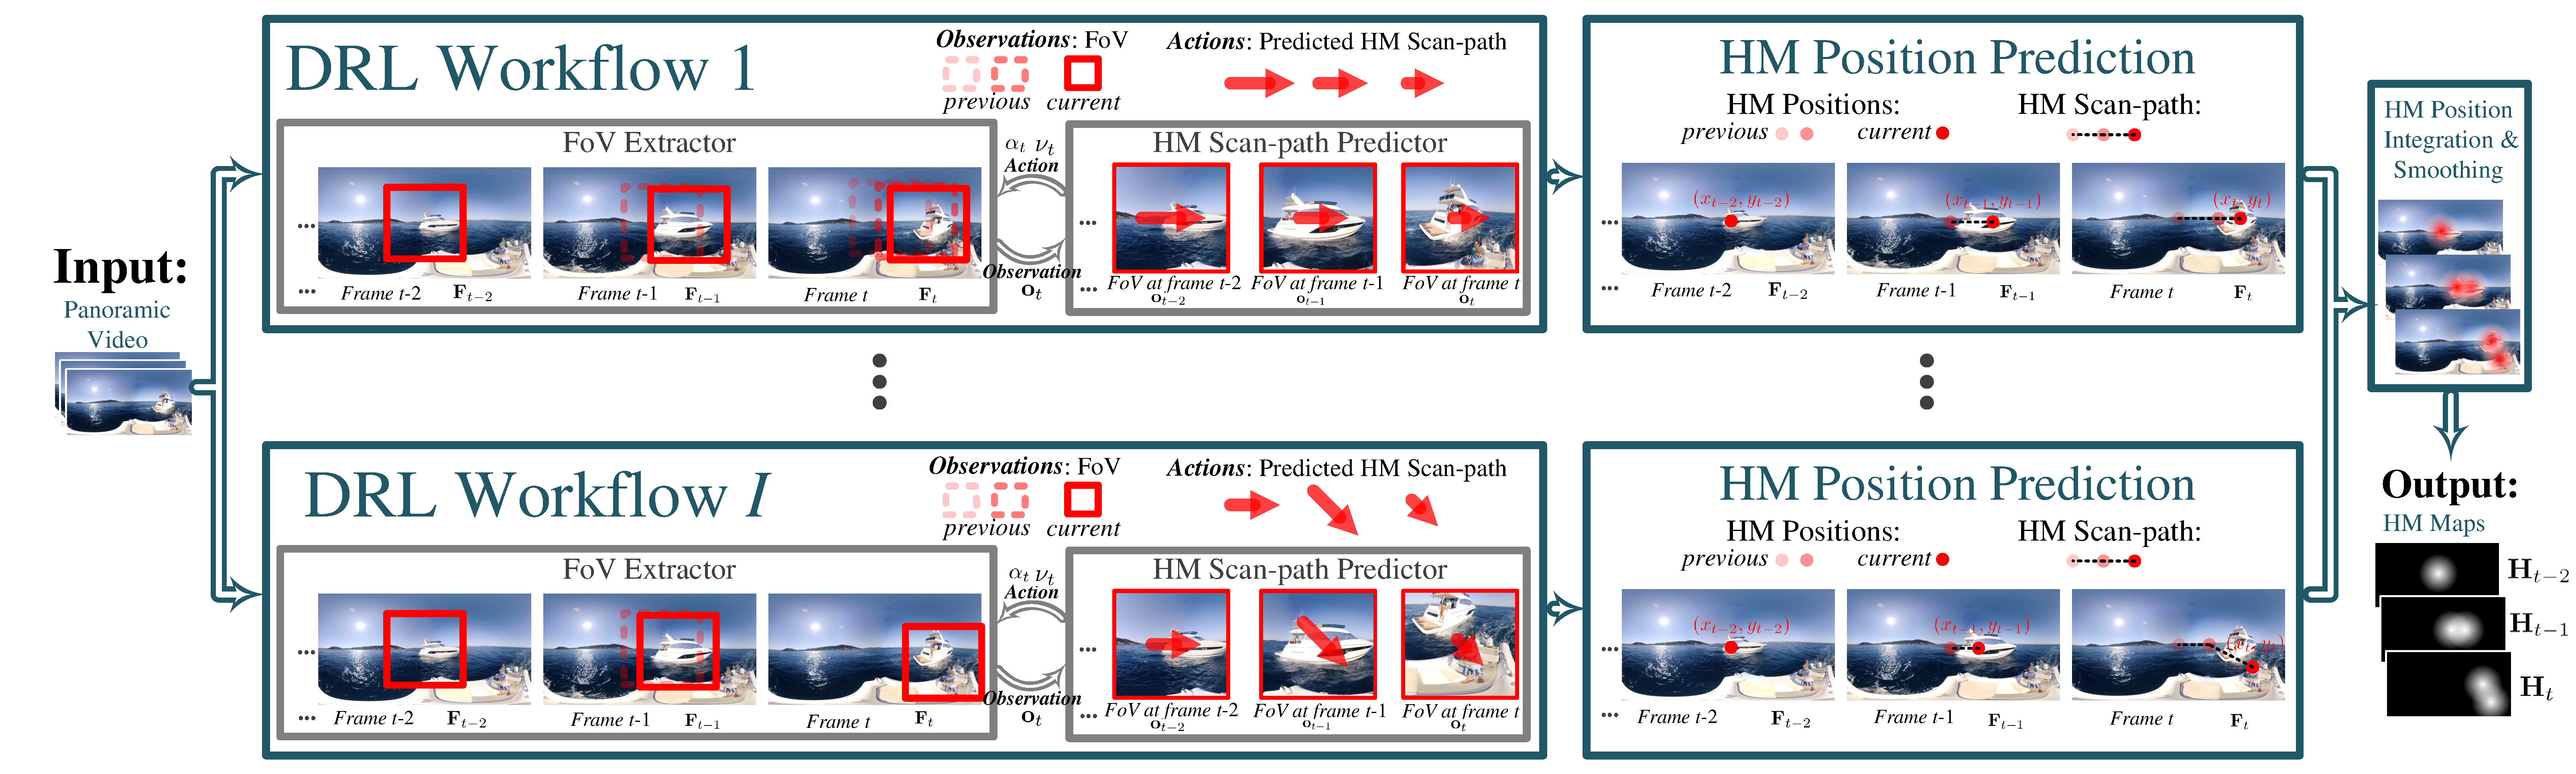
\includegraphics[width=2.0\columnwidth]{figures/dhp_approach/main_framework}}%of
        \vspace{-1em}
		\caption{\footnotesize{Overall framework of the offline-DHP approach.}}
		\label{main-framework}
	\end{center}
\vspace{-1em}
\end{figure*}

\begin{table*}
\vspace{-1em}
\center
\caption{Definitions of notations in the offline-DHP approach.} \label{notation_framework}
\vspace{-1em}
\begin{tabular}{ll}
%$\{t\}_{1}^{T}$ & The frames of panoramic video from $1$ to $T$, with $t$ being the currently processed frame \\
$\{\mathbf{F}_t\}_{t=1}^{T}$ & The panoramic frames with frame number $t$ ranging from $1$ to $T$, as the input to offline-DHP.\\
$\{\mathbf{H}_t\}_{t=1}^{T}$ & The HM maps for frames from $1$ to $T$, as the output of offline-DHP.\\
$\{m\}_{m=1}^{M}$ & The subjects from $1$ to $M$, with $m$ being the $m$-th subject.\\
$\{n\}_{n=1}^{N}$ & The DRL workflows from $1$ to $N$, with $n$ being the $n$-th workflow.\\
$\{\mathbf{o}^n_t\}_{t=1}^{T}$ & The FoVs for frames from $1$ to $T$, as the $observation$ of the $n$-th DRL workflow. \\
$(x^m_t, y^m_t)$ & The ground-truth HM position of the $m$-th subject at frame $t$. \\
$(\hat{x}^n_t, \hat{y}^n_t)$ & The HM position predicted by the $n$-th DRL workflow at frame $t$.  \\
%$(\mathbf{x}_t, \mathbf{y}_t)$ & The predicted HM position at frame $t$ \\
$\mathbf{\pi}_t$ & The predicted probability distribution of the HM direction at frame $t$, as the $policy$ of DRL. \\
$\hat{\alpha}^n_t$ & The predicted HM scanpath direction at frame $t$ from the $n$-th DRL workflow, as the $action$ of DRL.\\
$\alpha^m_t$ & The ground-truth HM scanpath direction of the $m$-th subject at frame $t$. \\
$\hat{\nu}^n_t$ & The predicted HM scanpath magnitude at frame $t$ from the $n$-th DRL workflow, also as the $action$ of DRL.\\
$\nu^m_t$ & The ground-truth HM scanpath magnitude of the $m$-th subject at frame $t$. \\
$r^{\alpha}_{n,t}$ & The \textit{reward} for deciding $\hat{\alpha}^n_t$ in the $n$-th DRL workflow.\\
$r^{\nu}_{n,t}$ & The \textit{reward} for deciding $\hat{\nu}^n_t$ in  the $n$-th DRL workflow.\\
$\mathbf{f}^n_{t}$ & The extracted LSTM feature at frame $t$,  as part of the \textit{observed state} in the $n$-th DRL workflow. \\
\end{tabular}
\vspace{-1em}
\end{table*}

\emph{Finding 5: Almost $50\%$ subjects are consistent in one HM scanpath direction (among 8 uniformly quantized directions), and over $85\%$ of subjects are consistent in three directions for HM scanpaths. }
\\ \textit{Analysis:} The distribution of HM scanpath directions in the PVS-HM database is analyzed as follows.
Only HM scanpaths falling into consistent HM regions (mentioned in \textit{Finding 4}) are selected for the analysis.
Specifically, we discretize continuous $0-360^{\circ}$ directions of HM scanpaths through 8-level uniform quantization: $\{0^{\circ}, 45^{\circ}, 90^{\circ} \cdots, 315^{\circ} \}$.
Then, we count the proportions of subjects whose HM scanpaths belong to the same discretized direction. Next, these proportions are ranked by their values in each extracted HM region, i.e., ranking from the 1-st to the 8-th. For each ranking, the proportions of subjects are averaged over all HM regions for each panoramic sequence, which are shown in Figure \ref{direction-consistence-distribution}.
As shown in this figure, for all 76 sequences, the HM scanpaths of $50\%$ subjects or more are consistent in the first ranked direction, and the HM scanpaths of over $85\%$ of subjects are consistent in top 3 directions. Figure \ref{direction-consistence-pie} also shows the proportions of subjects with HM scanpath directions ranking from the 1-st to the 8-th, which are averaged over all 76 sequences in the PVS-HM database.
As seen in this figure, the directions of the HM scanpaths from $57.1\%$, $20.6\%$ and $9.6\%$ subjects belong to the top 3 ranked directions. In contrast, the HM scanpath directions of $12.7\%$ of subjects fall into the other 5 directions. Therefore, \textit{Finding 5} is validated.





\emph{Finding 6: For one subject, the HM scanpath at the current time interval relies on that at the previous time interval and observed video content. }
\\ \textit{Analysis:} For each individual subject, the vectors of HM scanpaths across the time interval of 0.3 second are extracted from all 76 sequences in our PVS-HM database. Here, we calculate the CC values of HM scanpath vectors between two successive time periods, and then we average the CC values over all 76 sequences for each subject. Figure \ref{consi_on_time} shows the average CC values for each of the 58 subjects, which range from 0.39 - 0.51. This figure implies that the HM scanpath at the current time interval is somewhat correlated with that at the previous time interval. However, the CC value in Figure \ref{consi_on_time} is not sufficiently large, indicating that there exist other factors influencing the HM scanpath. Actually, \cite{hu2017deep} shows that the current HM scanpath of one subject is also related to the observed video content. The above completes the validation of \textit{Finding 6}.



%The relevance decreases when the time interval is increased.
%\emph{Finding 5: HM scanpath is predictable.The behavior of the next moment is of great relevance to the state of the last moment.We have proved that correlation between the direction of the next moment and the direction of this moment is more than $87.9\%$ (The longer the time interval, the smaller the correlation will be). }
%\\ \textit{Analysis:} We used the time interval as an independent variable,calculated the correlation between t and t-1,t-2... until t-10.The results are as follows.
%From \ref{consi_on_time} we can see that the first-order correlation of the HM scanpaths direction is $87.9\%$.This indicates that the HM scanpaths direction depends largely on the direction of the last moment.That is , each HM scanpaths direction is based on the HM scanpaths direction of the last moment.And the correlation coefficient decreases with the increase of order, indicating that the correlation will decrease with the time interval increase.
%As seen in this figure, First order correlation coefficient up to $87.9\%$,while the variance is only 0.023.



\section{Offline-DHP approach}\label{sec::offline-DHP}

\subsection{Framework of offline-DHP}
\label{framework}

In this section, we present our offline-DHP approach, in light of our findings in Section \ref{Database_analysis}.
Figure \ref{main-framework} shows the overall framework of our approach, in which the multiple DRL workflows are embedded to generate the HM maps of input panoramic video frames. The notations used in this figure and in our approach are listed in Table \ref{notation_framework}.





%$\mathbf{f}_{t-1}$ & LSTM feature produced by DRL model at frame $t-1$. $\mathbf{F}_t$ and $f_{t-1}$ compose a \textit{full observed state} of DRL $agent$ \\




As shown in Figure \ref{main-framework}, the input to our offline-DHP approach is the panoramic video frames $\{\mathbf{F}_t\}_1^{T}$.
Since \textit{Finding 2} has shown that the HM positions are highly consistent across different subjects,  we propose to generate the HM maps for modeling human attention on panoramic video, viewed as the output of our offline-DHP approach. The HM map $\mathbf{H}_t$ of frame $t$ represents the probability of each pixel being the HM position.
Similar to the saliency maps of 2D videos, $\mathbf{H}_t$ is obtained by convoluting the predicted HM positions $\{(\hat{x}^n_t, \hat{y}^n_t)\}_{n=1}^{N}$ with a 2D Gaussian filter.
Because \textit{Finding 5} has indicated that the HM scanpaths of different subjects are consistent in more than one direction, the HM positions $\{({x}^m_t, {y}^m_t)\}_{m=1}^{M}$ of $M$ subjects may be different from each other. Accordingly, this paper assumes that the number of predicted HM positions $N$ is equivalent to $M$ at each frame, for predicting the HM positions of all subjects.
In other words, to obtain $(\hat{x}^n_t, \hat{y}^n_t)$, our offline-DHP approach applies one DRL workflow to estimate the HM positions of one subject.
Then, $N$ DRL workflows are run to obtain $N$ HM positions $\{(\hat{x}^n_t, \hat{y}^n_t)\}_{n=1}^{N}$ at frame $t$, simulating the ground-truth HM positions of $M$ ($=N$) subjects at this frame.
At a panoramic frame, each of the DRL workflows works independently to generate an HM position by randomly sampling actions based on a learned policy $\pi_t$.
Note that all DRL workflows share the same policy $\pi_t$ in our approach.

In a single DRL workflow , $\{(\hat{x}^n_t, \hat{y}^n_t)\}_{t=1}^T$ can be modeled by determining a series of \textit{actions}: $\{\hat{\alpha}^n_t\}_{t=1}^T$ and $\{\hat{\nu}^n_t\}_{t=1}^T$.
It is worth pointing out that $\{\hat{\alpha}^n_t\}_{t=1}^{T}$ and $\{\hat{\nu}^n_t\}_{t=1}^{T}$ are predictable as the \textit{actions} of the DRL workflow, since \textit{Findings 3} and \textit{4} have indicated that subjects are consistent in the magnitudes and directions of HM scanpaths.
As can be seen in Figure \ref{main-framework}, in each workflow, one HM scanpath is generated through the interaction between the FoV extractor\footnote{Note that the extracted FoV is $103^{\circ} \times 60^{\circ}$, which is the same as the setting of the HMD.} and HM scanpath predictor.
Specifically, Figure \ref{main-framework} shows that FoV $\mathbf{o}^n_t$ is extracted via making its center locate at the HM position $(\hat{x}^n_t,\hat{y}^n_t)$, in which $(\hat{x}^n_t,\hat{y}^n_t)$ is generated by the predicted \textit{action} of HM scanpaths $(\hat{\alpha}^n_{t-1},\hat{\nu}^n_{t-1})$ at the previous video frame.
Then, the content of the extracted FoV works as the \textit{observation} of DRL, for predicting the next \textit{action} of HM scanpath $(\hat{\alpha}^n_{t},\hat{\nu}^n_{t})$.
The HM scanpath generated by each DRL workflow is forwarded to obtain HM positions at incoming frames.
Subsequently, the HM positions from multiple DRL workflows are integrated, and then smoothed by a 2D Gaussian filter.
Finally, the HM maps $\{\mathbf{H}_t\}_1^{T}$ of the panoramic video are obtained, which model the heat maps for the HM positions at each frame.

%Assuming that $p^n(x_t,y_t)$ is the probability of the $n$-th subject's HM position being at $(x_t,y_t)$, $p(x_t,y_t)$ can be estimated by the following expectation:
% \begin{equation}\label{define-hm-maps}
%   p(x_t,y_t) = \mathbb{E}\{ p^n(x_t, y_t) \}.
% \end{equation}
%
%To obtain $ p^n(x_t, y_t)$, our offline-DHP approach estimates the HM positions of one subject through HM scanpath prediction of one DRL workflow. In fact, $p^n(x_t, y_t)$ of \eqref{define-hm-maps} can be modeled by determining a series of \textit{actions} in the DRL workflow: $\alpha_1,\alpha_2,...,\alpha_t$ and $\nu_1,\nu_2,...,\nu_t$. It is worth pointing out that it is reasonable to model $\{\alpha_t\}_{t=1}^{T}$ and $\{\nu_t\}_{t=1}^{T}$ as the \textit{actions} in the DRL workflow, since \textit{Findings 2} and \textit{3} have indicated that subjects are consistent in the magnitudes and directions of HM scanpaths.

%Since \textit{Finding 4} has found that the HM scanpaths of different subjects are consistent in more than one directions, it is impossible to model $p(x_t,y_t)$ of \eqref{define-hm-maps} through $p^n(x_t, y_t)$ of only one DRL workflow.
%Instead, the HM map can be generated by running $N$ DRL workflows to calculate $p(x_t,y_t)$ with \eqref{define-hm-maps}.
%More specifically, our offline-DHP method runs multiple DRL workflows, each of which works independently to generate a HM scanpath by random sampling actions based on a learnt policy $\pi_t$.
%The generated HM scanpaths of all DRL workflows are then integrated to produce the HM map upon the expectation of HM positions in \eqref{define-hm-maps}.



%\begin{proposition}
%    \label{lemma2}
%      $\mathbb{E}$ in \eqref{define-hm-maps} can be modeled by running multiple DRL workflows, given a learned HM scanpath predictor.
%        \begin{eqnarray}
%        \label{proposition_2}
%        && \mathbb{E}\{ p^n(x_t, y_t) \} \nonumber\\
%        &=& \mathbb{E}_{\pi(x_{t},y_{t} |\Psi_{ x_{t-1}, y_{t-1} } ),...,\pi(x_{2},y_{2} |\Psi_{ x_{1}, y_{1} } )} \{ \mathbb{E} \{ p^n( \Psi_{ x_{1}, y_{1} } ) \} \}.
%        \end{eqnarray}
%
%    \textbf{Proof:}
%        Since \textit{Findings 2-4} have revealed that $\alpha^n_t$ and $\nu^n_t$ are generally consistent across different $n$, we assume that $p(\alpha_{t-1}, \nu_{t-1} | \Psi_{ x_{t-1}, y_{t-1} } )$ of all subjects is with the same probability distribution, denoted by $\pi(x_{t},y_{t}|\Psi_{x_{t-1}, y_{t-1} } )$. That is,
%        \begin{eqnarray}
%        \label{p-sim-pi}
%        p( \alpha_{t-1}, \nu_{t-1} | \Psi_{ x_{t-1}, y_{t-1} } ) \sim \pi(x_{t},y_{t} | \Psi_{ x_{t-1}, y_{t-1} } ).
%        \end{eqnarray}
%        Thus, based on \eqref{expand-define-with-full-prob-formula} and \eqref{p-sim-pi}, the expectation of \eqref{use-define-of-expectation} can be rewritten in the following,
%        \begin{eqnarray}
%        \label{use-define-of-expectation1}
%        && \mathbb{E}\{ p^n(x_t, y_t) \} \nonumber\\
%        \nonumber &=& \mathbb{E}\{ p^n(\Psi_{ x_t, y_t }) \} \nonumber\\
%        &=& \mathbb{E}_{\pi(x_{t},y_{t} |\Psi_{ x_{t-1}, y_{t-1} } ) } \{ \mathbb{E} \{ p^n( \Psi_{ x_{t-1}, y_{t-1} } ) \} \}.
%        \end{eqnarray}
%         Above \eqref{use-define-of-expectation1} can be iterated till $p^n( \Psi_{ x_{1}, y_{1} } )$, which derives \eqref{proposition_2} in Proposition 2.
%
%\end{proposition}


\subsection{DRL model of the offline-DHP approach}
\label{train}
As described in Section \ref{framework}, the DRL workflow is a key component in our offline-DHP framework, which targets at predicting the HM scanpaths.
This section presents how to train the DRL model of each workflow for predicting the HM maps.
In this section, we take the $n$-th workflow as an example.
Figure \ref{train-framework} shows the framework of training the DRL model.
As shown in this figure, the FoV of the input video frame is extracted based on the \textit{action} of the HM scanpath predicted at the previous frame.
The extracted FoV, as the \textit{observation}, is then fed into the DRL network.
In addition, the \textit{reward}, which measures the similarity between the predicted and ground-truth HM scanpaths, is estimated to evaluate the \textit{action} made by the DRL model. Then, the \textit{reward} is used to make decision on the \textit{action} through the DRL model, i.e., the HM scanpath at the current frame.
Finally, the \textit{environment} of our DRL model is comprised by the \textit{observation} of the extracted FoV and the \textit{reward} of HM scanpath prediction.

In training the DRL model,  the \textit{environment} interacts with the HM scanpath predictor.
The interaction is achieved in our DRL model through the following procedure.\\
(1) At frame $t$, the FoV extractor obtains the current $\textit{observation}$ $\mathbf{o}^n_t$ ($103^{\circ} \times 60^{\circ}$) from the input video frame $\mathbf{F}_t$, according to the predicted HM position $(\hat{x}^n_t,\hat{y}^n_t)$.
In our work, $\mathbf{o}^n_{t}$ is projected onto the 2D region and is then down-sampled to $42\times42$.\\
(2) The current $\mathbf{o}^n_t$ and the LSTM feature $\mathbf{f}^n_{t-1}$ from  the last frame are delivered to the DRL network in the HM scanpath predictor.
In our work, the DRL network contains four convolutional layers and one LSTM layer \cite{hausknecht2015deep}, which are used to extract the spatial and temporal features, respectively. The details about the architecture of the DRL network can be found in Figure \ref{train-framework}.\\
(3) At frame $t$, the DRL network produces the LSTM feature $\mathbf{f}^n_{t}$, HM scanpath magnitude $\hat{\nu}^n_{t}$ and policy $\pi_{t}$. Here, $\pi_{t}$ is modeled by the probability distribution over the \textit{actions} of HM scanpath directions.\\
(4) Given $\pi_{t}$, the HM scanpath predictor randomly samples an \textit{action} $\hat{\alpha}^n_t$ with standard deviation $\varepsilon$, such that the exploration is ensured in decision making. Here, $\hat{\alpha}^n_t$ includes 8 discrete directions in GDS: $\{ 0^{\circ}, 45^{\circ}, \cdots, 315^{\circ} \}$.\\
(5) \textit{Environment} is updated using $\hat{\nu}^n_t$ and $\hat{\alpha}^n_t$, leading to $(\hat{x}^n_t, \hat{y}^n_t)\longrightarrow (\hat{x}^n_{t+1},\hat{y}^n_{t+1})$. The FoV extractor returns a new \textit{observation} $\mathbf{o}^n_{t+1}$ according to the HM position $(\hat{x}^n_{t+1},\hat{y}^n_{t+1})$. The \textit{reward} estimator returns the \textit{rewards} $r^{\nu}_{n,t}$ and $r^{\alpha}_{n,t}$ in predicting $\hat{\nu}^n_t$ and $\hat{\alpha}^n_t$, based on the ground-truth HM scanpaths of $\{\nu^m_t\}_{m=1}^{M}$ and $\{\alpha^m_t\}_{m=1}^{M}$. \\
(6) A set of experiences $\{ \mathbf{o}^n_{t}, \! \mathbf{f}^n_{t-1},\! \hat{\nu}^n_t,\! \hat{\alpha}^n_t,\! r^{\nu}_{n,t},\! r^{\alpha}_{n,t} \}$ are stored in an experience buffer for frame $t$.
In addition, $\mathbf{o}^n_{t+1}$ and $\mathbf{f}^n_{t}$ are preserved for processing frame $t+1$.\\
(7) Once $t$ meets the termination condition of exceeding the maximum frame number $T$, all experiences in the buffer are delivered to the optimizer for updating the DRL network.


\begin{figure*}
	\begin{center}
		\centerline{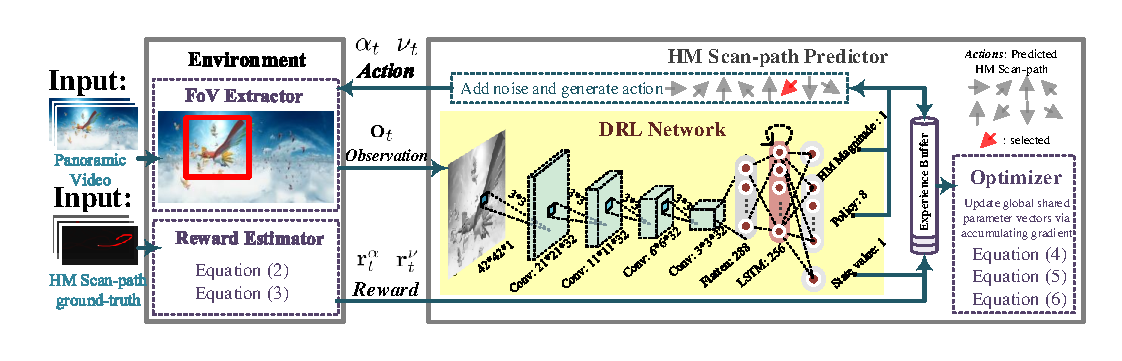
\includegraphics[width=1.5\columnwidth]{figures/dhp_approach/training_framework}}%of
		\caption{\footnotesize{Framework of training the DRL model to obtain each DRL workflow of the offline-DHP approach (Figure \ref{main-framework}).}}
		\label{train-framework}
	\end{center}
\end{figure*}

\textbf{Reward Estimation.}
Next, we focus on modeling the \textit{rewards} $r^{\alpha}_{n,t}$ and $r^{\nu}_{n,t}$ in determining the \textit{actions} of HM scanpaths.
When training the DRL model, our goal is to make the prediction of $\hat{\alpha}^n_{t}$ and $\hat{\nu}^n_{t}$ approach the ground-truth HM scanpaths.
Thus, the  \textit{rewards} $r^{\alpha}_{n,t}$ and $r^{\nu}_{n,t}$ can be represented by the differences from $\hat{\alpha}^n_{t}$  to $\{{\alpha}^m_{t}\}_{m=1}^M$ and from $\hat{\nu}^n_{t}$ to $\{{\nu}^m_{t}\}_{m=1}^M$, respectively.
In our approach, these differences are measured by Gaussian distributions.
%we use the Gaussian distribution to measure the differences between $\hat{\alpha}^n_{t}$ and the ground-truth $\{\alpha^{m}_{t}\}_{m=1}^M$ and between $\hat{\nu}^n_{t}$ and $\{{\nu}^m_{t}\}_{m=1}^M$.
We further consider the distances from predicted HM position $(\hat{x}^n_t,\hat{y}^n_t)$ to $\{(x^{n}_{t},y^{n}_{t})\}_{m=1}^M$ in calculating the \textit{rewards} of $r^{\alpha}_{n,t}$ and $r^{\nu}_{n,t}$, which are also modeled by the 2D Gaussian distribution.
This consideration is because only the consistent HM regions have similar HM scanpaths, according to the analysis of \textit{Finding 4}.
Then, $r^{\alpha}_{n,t}$ can be written as
\begin{equation}
\label{reward-alpha}
r^{\alpha}_{n,t} = \frac{1}{N}\sum_{m=1}^{M} e^{-\frac{1}{2}\left(\frac{D_d(\hat{\alpha}^n_{t}, \alpha^m_{t})}{\rho}\right)^2} e^{-\frac{1}{2}\left(\frac{D_s((\hat{x}^n_{t},\hat{y}^n_{t}),(x^m_{t},y^m_{t}))}{\varrho}\right)^2},
\end{equation}
In \eqref{reward-alpha}, $D_d$ defines the phase difference, and $D_s$ denotes the great-circle distance \cite{shumaker1984astronomical}. Moreover, $\rho$ and $\varrho$ are the standard deviations of Gaussian distributions, as the hyper-parameters. Similarly, we have
\begin{equation}
\label{reward-nu}
r^{\nu}_{n,t} \!\!=\!\! \frac{1}{N}\!\sum_{m=1}^{M}\!
e^{\!-\frac{1}{2}\left(\!{\frac{\hat{\nu}^n_{t}-\nu^{m}_{t}}{\varsigma}}\!\right)^2} \! e^{\!-\frac{1}{2}\left(\!\frac{D_d(\hat{\alpha}^n_{t}, \alpha^m_{t})}{\rho}\!\right)^2} \!\!e^{\!-\frac{1}{2}\left(\!\frac{D_s((\hat{x}^n_{t},\hat{y}^n_{t}),(x^m_{t},y^m_{t}))}{\varrho}\!\right)^2}.
\end{equation}
where $\varsigma$ is the hyper-parameter for the standard deviation of the HM scanpath magnitude.


%\begin{proposition}
%    \label{lemma3}
%    Assume that probability $p(x_t,y_t)$ decays along with the distance of $(x_t,y_t)$ to the ground-truth HM position $(x^{n}_{t},y^{n}_{t})$, obeying the 2D Gaussian distribution.
%    Additionally, assume that the probability of $\alpha_{t}$ also follows the Gaussian distribution with the mean being $\alpha^{n}_{t}$.
%    Then, $r^{\alpha}_t$ can be represented by \eqref{reward-alpha}.
%
%    \textbf{Proof:} At frame $t$, the ground-truth HM position is $\{x^{n}_{t},y^{n}_{t} \}$ for  the $n$-th subject.
%    Besides, $\alpha^{n}_{t}$ is the  ground-truth direction of HM scanpath for the $n$-th subject.
%    Thus, we can acquire:
%    \begin{eqnarray}
%        \label{reward-Pro10}
%        && P(\alpha^{n}_{t}|(x^{n}_{t}, y^{n}_{t})) = 1.
%        %\label{reward-Pro2}
%%        && P(\nu^{n}_{t}|\{x^{n}_{t}, y^{n}_{t}\},\alpha^{n}_{t}) = 1
%    \end{eqnarray}
%    Since the probability of $(x_{t},y_{t})$ being the HM position follows Gaussian distribution centered at $(x^{n}_{t},y^{n}_{t})$, the equality below can be obtained:
%    \begin{equation}
%        \label{reward-Pro11}
%        P_{n}(\alpha^{n}_{t}|(x_{t},y_{t})) = P_{n}(\alpha^{n}_{t}|(x^n_{t},y^n_{t})) e^{-\frac{1}{2}\left(\frac{D_s((x_{t},y_{t}),(x^n_{t},y^n_{t}))}{\varrho}\right)^2}.
%    \end{equation}
%    Similarly, we have
%    \begin{eqnarray}
%        \label{reward-Pro12}
%        P_{n}(\alpha_{t}|(x_{t},y_{t})) = P_{n}(\alpha^{n}_{t}|(x_{t},y_{t})) e^{-\frac{1}{2}\left(\frac{D_d(\alpha_{t}, \alpha^n_{t})}{\rho}\right)^2}.
%    \end{eqnarray}
%    Based on \eqref{reward-Pro11}, we can rewrite \eqref{reward-Pro12} as
%    \begin{eqnarray}
%        \label{reward-Pro5}
%        \nonumber && P_{n}(\alpha_{t}|(x_{t},y_{t})) = P_{n}(\alpha^{n}_{t}|(x^{n}_{t}, y^{n}_{t})) \cdot \\ && e^{-\frac{1}{2}\left(\frac{D_s((x_{t},y_{t}),(x^n_{t},y^n_{t}))}{\varrho}\right)^2}
%        e^{-\frac{1}{2}\left(\frac{D_d(\alpha_{t}, \alpha^n_{t})}{\rho}\right)^2}.
%    \end{eqnarray}
%   Because of \eqref{reward-Pro10}, the following holds:
%    \begin{equation}
%        \label{reward-Pro6}
%        P_{n}(\alpha_{t}|(x_{t},y_{t}))\!=\! e^{-\frac{1}{2}\left(\frac{D_d(\alpha_{t}, \alpha^n_{t})}{\rho}\right)^2}\! e^{-\frac{1}{2}\left(\frac{D_s((x_{t},y_{t}),(x^n_{t},y^n_{t}))}{\varrho}\right)^2}.
%    \end{equation}
%    Reward $r^{\alpha}_t$ can be represented by $P_{n}(\alpha_{t}|(x_{t},y_{t}))$ averaged overall subjects, i.e., \eqref{reward-alpha}, which calculates how likely the subjects conduct the action of $\alpha_{t}$. Finally, this proposition is proved.
%\end{proposition}



%\begin{proposition}
%    \label{lemma3}
%    Assume that the probability of each pixel $\{\hat{x}_{t},\hat{y}_{t}\}$ being the HM position decays along with the distance to the ground truth HM position, following 2D coordinate Gaussian distribution \textcolor{blue}{along with longitude and latitude}.
%    In addition, assume that the probability for the degree $\alpha^{n}_{t}$ of HM scan path also follows the Gaussian distribution with the mean being $\alpha^{n}_{t}$.
%    Then $r^{\alpha}_t$ can be represented by \eqref{reward-alpha}.
%
%    \textbf{Proof:} At frame $t$, the ground truth HM position is $\{x^{n}_{t},y^{n}_{t} \}$ for  the $n$-th subject.
%    besides, $\alpha^{n}_{t}$ is the direction of HM scan path for the $n$-th subject.
%    Thus, we can acquire:
%    \begin{eqnarray}
%        \label{reward-Pro1}
%        && P(\alpha^{n}_{t}|\{x^{n}_{t}, y^{n}_{t}\}) = 1.
%        %\label{reward-Pro2}
%%        && P(\nu^{n}_{t}|\{x^{n}_{t}, y^{n}_{t}\},\alpha^{n}_{t}) = 1
%    \end{eqnarray}
%    Since the probability of $\{\hat{x}_{t},\hat{y}_{t}\}$ being the HM position follows Gaussian distribution centered at $\{x^{n}_{t},y^{n}_{t} \}$, the equality below can be obtained:
%    \begin{equation}
%        \label{reward-Pro3}
%        P_{n}(\alpha^{n}_{t}|\{\hat{x}_{t},\hat{y}_{t}\}) = P_{n}(\alpha^{n}_{t}|\{x^{n}_{t}, y^{n}_{t}\}) e^{-\frac{1}{2}\left(\frac{D_s((\hat{x}_{t},\hat{y}_{t}),(x^n_{t},y^n_{t}))}{\varrho}\right)^2}.
%    \end{equation}
%    Similarly, we have:
%    \begin{eqnarray}
%        \label{reward-Pro4}
%        P_{n}(\hat{\alpha}_{t}|\{\hat{x}_{t},\hat{y}_{t}\}) = P_{n}(\alpha^{n}_{t}|\{\hat{x}_{t},\hat{y}_{t}\}) e^{-\frac{1}{2}\left(\frac{D_d(\hat{\alpha}_{t}, \alpha^n_{t})}{\rho}\right)^2}.
%    \end{eqnarray}
%    Based on \eqref{reward-Pro3}, \eqref{reward-Pro4} can be written as:
%    \begin{eqnarray}
%        \label{reward-Pro5}
%        \nonumber && P_{n}(\hat{\alpha}_{t}|\{\hat{x}_{t},\hat{y}_{t}\}) = P_{n}(\alpha^{n}_{t}|\{x^{n}_{t}, y^{n}_{t}\}) \cdot \\ && e^{-\frac{1}{2}\left(\frac{D_s((\hat{x}_{t},\hat{y}_{t}),(x^n_{t},y^n_{t}))}{\varrho}\right)^2}
%        e^{-\frac{1}{2}\left(\frac{D_d(\hat{\alpha}_{t}, \alpha^n_{t})}{\rho}\right)^2}.
%    \end{eqnarray}
%    According to \eqref{reward-Pro1}, the following holds:
%    \begin{equation}
%        \label{reward-Pro6}
%        P_{n}(\hat{\alpha}_{t}|\{\hat{x}_{t},\hat{y}_{t}\}) = e^{-\frac{1}{2}\left(\frac{D_d(\hat{\alpha}_{t}, \alpha^n_{t})}{\rho}\right)^2} e^{-\frac{1}{2}\left(\frac{D_s((\hat{x}_{t},\hat{y}_{t}),(x^n_{t},y^n_{t}))}{\varrho}\right)^2}.
%    \end{equation}
%    Reward $r^{\alpha}_t$ can be represented by $P_{n}(\hat{\alpha}_{t}|\{\hat{x}_{t},\hat{y}_{t}\})$ averaged overall subjects, i.e., \eqref{reward-alpha},which estimates how likely human agent conducts the action of $\hat{\alpha}_{t}$. Finally, this proposition is proved.
%\end{proposition}

%\begin{proposition}
%    \label{lemma4}
%    Assume that the probability of each pixel $\{\hat{x}_{t},\hat{y}_{t}\}$ being the HM position decays along with the distance to the ground truth HM position, following 2D coordinate Gaussian distribution \textcolor{blue}{along with longitude and latitude}.
%    In addition, assume that the probability for the degree $\alpha^{n}_{t}$ of HM scan path also follows the Gaussian distribution with the mean being $\alpha^{n}_{t}$.
%    Then $r^{\alpha}_t$ can be represented by \eqref{reward-alpha}.
%    Provided that the probability for the magnitude $\hat{\nu}_{t}$ of HM scan path follows the Gaussian distribution with the mean of $\nu^{n}_{t}$.
%    We have \eqref{reward-nu}.
%
%    \textbf{Proof:} At frame $t$, $\nu^{n}_{t}$ is the magnitude of HM scan path at the direction $\alpha^{n}_{t}$ for the $n$-th subject.
%    Then, similar to the proof of \eqref{reward-Pro1}, the following holds:
%    \begin{equation}
%        \label{mu-Pro1}
%        P(\nu^{n}_{t}|\{x^{n}_{t}, y^{n}_{t}\},\alpha^{n}_{t}) = 1.
%    \end{equation}
%    \begin{eqnarray}
%        \label{mu-Pro2}
%        \nonumber && P_{n}(\nu^{n}_{t}|\{\hat{x}_{t},\hat{y}_{t}, \hat{\alpha}_{t}\}) = P(\nu^{n}_{t}|\{x^{n}_{t}, y^{n}_{t}\},\alpha^{n}_{t}) \cdot \\ && e^{-\frac{1}{2}\left(\frac{D_s((\hat{x}_{t},\hat{y}_{t}),(x^n_{t},y^n_{t}))}{\varrho}\right)^2}
%        e^{-\frac{1}{2}\left(\frac{D_d(\hat{\alpha}_{t}, \alpha^n_{t})}{\rho}\right)^2}.
%    \end{eqnarray}
%    Due to the Gaussian distribution of the probability for magnitude $\hat{\nu}_{t}$, we can obtain:
%    \begin{eqnarray}
%        \label{mu-Pro3}
%        \nonumber && P_{n}(\nu^{n}_{t}|\{\hat{x}_{t},\hat{y}_{t}, \hat{\alpha}_{t}\})\\
%        \nonumber &=& P(\nu^{n}_{t}|\{x^{n}_{t}, y^{n}_{t}\},\alpha^{n}_{t})
%        e^{-\frac{1}{2}\left({\hat{\nu}_{t}-\nu^{n}_{t}}\right)^2} \cdot \\ &&
%        e^{-\frac{1}{2}\left(\frac{D_s((\hat{x}_{t},\hat{y}_{t}),(x^n_{t},y^n_{t}))}{\varrho}\right)^2}
%        e^{-\frac{1}{2}\left(\frac{D_d(\hat{\alpha}_{t}, \alpha^n_{t})}{\rho}\right)^2}.
%    \end{eqnarray}
%    According to \eqref{mu-Pro1} and \eqref{mu-Pro3}, we have:
%    \begin{eqnarray}
%        \label{mu-Pro4}
%        \nonumber && P_{n}(\nu^{n}_{t}|\{\hat{x}_{t},\hat{y}_{t}, \hat{\alpha}_{t}\}) =
%        e^{-\frac{1}{2}\left({\hat{\nu}_{t}-\nu^{n}_{t}}\right)^2} \cdot \\ &&
%        e^{-\frac{1}{2}\left(\frac{D_s((\hat{x}_{t},\hat{y}_{t}),(x^n_{t},y^n_{t}))}{\varrho}\right)^2}
%        e^{-\frac{1}{2}\left(\frac{D_d(\hat{\alpha}_{t}, \alpha^n_{t})}{\rho}\right)^2}.
%    \end{eqnarray}
%    Reward $r^{\nu}_{t}$ can be similarly represented by
%    $P(\nu^{n}_{t}|\{x^{n}_{t}, y^{n}_{t}\},\alpha^{n}_{t})$ averaged overall subjects, i.e., \eqref{reward-nu}.
%    This completes the proof of proposition 4.
%\end{proposition}

\textbf{Optimization.}
Next, we need to optimize the \textit{rewards} $r^{\alpha}_{n,t}$ and $r^{\nu}_{n,t}$, when learning the network parameters of our DRL model in Figure \ref{train-framework}.
Our offline-DHP approach applies the asynchronous DRL method \cite{mnih2016asynchronous} to learn the DRL parameters with optimized \textit{rewards}.
Hence, multiple workflows are run to interact with multiple \textit{environments} with workflow-specific parameter vectors $\{ \theta^{n}_{\nu}, \theta^{n}_{\pi}, \theta^{n}_{V} \}$, producing $\hat{\nu}^n_t$, $\hat{\pi}^n_t$ and $V$.
Here, $V$ denotes the \textit{state value} output by the DRL network, which is obtained using the same way as \cite{mnih2016asynchronous}.
Meanwhile, global-shared parameter vectors $\{ \theta_{\nu}, \theta_{\pi}, \theta_{V} \}$\footnote{As can be seen in Figure \ref{train-framework}, $\{ \theta_{\nu}, \theta_{\pi}, \theta_{V} \}$ share all CNN and LSTM layers in our offline-DHP approach, but they are separated at the output layer.} are updated via an accumulating gradient.
For more details about the workflow-specific and global-shared parameter vectors, refer to \cite{mnih2016asynchronous}.
In our approach, \textit{reward} $r^{\nu}_{n,t}$ is optimized to train $\theta_{\nu}$ as follows:
\begin{equation}
\label{opt-1}
d \theta_{\nu} \leftarrow d \theta_{\nu} + \nabla_{\theta_{\nu}^{n}} \sum_{t=1}^{T} r^{\nu}_{n,t}.
\end{equation}
Moreover, we can optimize \textit{reward} $r^{\alpha}_{n,t}$ by
\begin{equation}
\label{opt-2}
\small d \theta_{V} \leftarrow d \theta_{V} + \nabla_{\theta_{V}^{n}} \sum_{t = 1}^{T} (\sum_{i=t}^{T} \gamma^{i-t} r^{\alpha}_{n,i} - V(\mathbf{o}^n_{t}, \mathbf{f}^n_{t-1} ; \theta_{V}^{n}))^2,
\end{equation}
\begin{small}
\begin{eqnarray}
\label{opt-3}
\hspace{0.1cm} \nonumber d \theta_{\pi} \leftarrow d \theta_{\pi} +\nabla_{\theta_{\pi}^{n}} \sum_{t = 1}^{T} \log \pi( \hat{\alpha}^n_{t} | \mathbf{o}^n_{t}, \mathbf{f}^n_{t-1} ; \theta_{\pi}^{n})\cdot \\
(\sum_{i = t}^{T} \gamma^{i-t} r^{\alpha}_{n,i} - V(\mathbf{o}^n_{t}, \mathbf{f}^n_{t-1} ; \theta_{V}^{n})),
\end{eqnarray}
\end{small}
where $\gamma$ is the discount factor of \textit{Q-learning} \cite{watkins1992q}.
In addition, $V(\mathbf{o}^n_{t}, \mathbf{f}^n_{t-1} ; \theta_{V}^{n})$ denotes state value $V$ obtained by $\mathbf{o}^n_{t}, \mathbf{f}^n_{t-1}$ and $\theta_{V}^{n}$; $\pi( \hat{\alpha}^n_{t} | \mathbf{o}^n_{t}, \mathbf{f}^n_{t-1} ; \theta_{\pi}^{n})$ stands for the probability of \textit{action} $\hat{\alpha}^n_{t}$ that is made by policy $\pi_t$ from $\mathbf{o}^n_{t}, \mathbf{f}^n_{t-1}$ and $\theta_{\pi}^{n}$.
Finally, based on the above equations, RMSProp \cite{tieleman2012lecture} is applied to optimize \textit{rewards} in the training data. Consequently, the workflow-specific and global-shared parameter vectors can be learned to predict HM scanpaths.
Finally, these learned parameter vectors can be used to determine the scanpaths and positions of HM through each DRL workflow in our offline-DHP approach.

\section{Online-DHP approach}

\begin{figure}
\vspace{-2em}
	\begin{center}
		\centerline{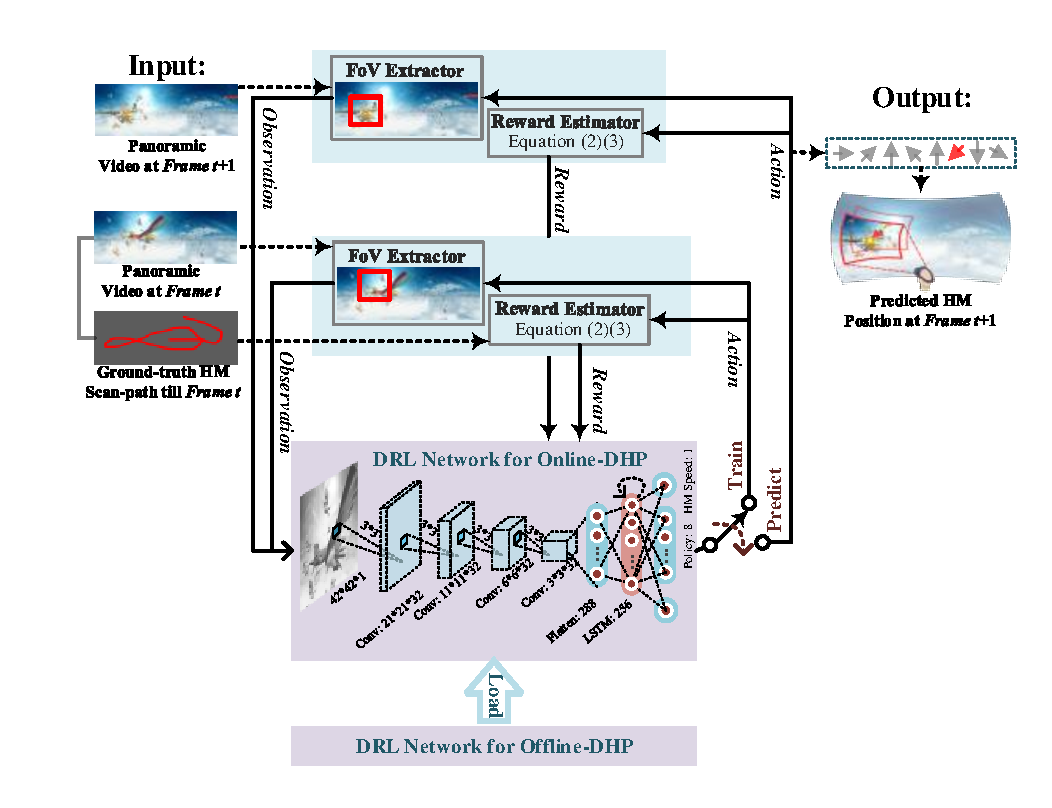
\includegraphics[width=\columnwidth]{figures/dhp_approach_on_line/whole_framework_online_5}}%of
       \vspace{-1em}
		\caption{\footnotesize{Framework of the online-DHP approach.}}
		\label{online-framework}
	\end{center}
\vspace{-2em}
\end{figure}

In this section, we present our online-DHP approach.
The online-DHP approach refers to predicting a specific subject's HM position $(\hat{x}_{t+1},\hat{y}_{t+1})$ at frame $t+1$, given his/her HM positions $\{(x_{1},y_{1}),\ldots, (x_{t},y_{t})\}$ till frame $t$.
Note that the definitions of the notations in this section are similar to those in Section \ref{sec::offline-DHP}, and the only difference is that $n$ and $m$ are removed in all notations because there is only one subject/workflow in online-DHP.
Additionally, we define the subject as the \textit{viewer}, whose HM positions need to be predicted online. % online viewer
Figure \ref{online-framework} shows the framework of our online-DHP approach. %, which predicts the HM position $(x_{t+1},y_{t+1})$ upon observation $\{\mathbf{o}_1, \ldots, \mathbf{o}_t\}$ till frame $t$.
According to \textit{Finding 6}, the current HM scanpath is correlated with the previous HM scanpaths and the video content.
Therefore, the input to our online-DHP framework is the \textit{viewer's} HM scanpath $\{(\alpha_1,\nu_1),\ldots, (\alpha_{t-1},\nu_{t-1})\}$ and frame content $\{\mathbf{F}_1, \ldots, \mathbf{F}_t \}$, and the output is the predicted HM position $(\hat{x}_{t+1},\hat{y}_{t+1})$ at the next frame for the \textit{viewer}.
This can be viewed as online prediction of HM positions $\{(\hat{x}_{t},\hat{y}_{t})\}_{t=1}^{T}$ .
To this end, our online-DHP consists of two stages: the training and prediction stages.
In the first stage, the parameters of the DRL network are trained.
In the second stage, the \textit{action} of the HM scanpath is generated from the trained DRL network, to predict the HM position online.
In the following, we discuss these two stages in more detail.

\subsection{Stage I: Training}
At the beginning frame, the HM position $(\hat{x}_1,\hat{y}_1)$ of the \textit{viewer} is initialized to be the center of the front region, which is the general setting of  the panoramic video player. Then, the trained DRL network of offline-DHP is loaded as the initial DRL network for online prediction, both sharing the same structure.
The reason for loading the offline-DHP network is that it encodes the knowledge of HM-related features.
Later, this initial DRL network is fine-tuned by the \textit{viewer's} HM scanpath at incoming frames.

Next, we focus on the algorithm for training the DRL network in our online-DHP approach. As previously mentioned, the initial parameters of the DRL network at the first frame are directly from those of offline-DHP. At each of the incoming frames, several episodes are run to update the DRL network for online-DHP. The following summarizes the procedure of one episode at frame $t+1$.

%As aforementioned, the offline DRL network is loaded in the initialization of our online-DHP approach. Thus, training the DRL network for online-DHP generally follows that of offline-DHP, both containing the basic reinforcement learning procedure. XXX.
%To predict the HM position of
%
%The following shows the procedure of one episode,
\begin{enumerate}
  \item Iterate the following steps from $i=1$ to $t$. At each iteration, $(\hat{\alpha}_i,\hat{\nu}_i)$ and $(\alpha_i,\nu_i)$ are the predicted and ground-truth \textit{actions}, respectively, of the HM scanpath for the \textit{viewer}, and $\mathbf{o}_i$ is the \textit{observation} of the FoV content.
  \item Take the \textit{action} of $(\hat{\alpha}_i,\hat{\nu}_i)$ using the DRL network, given the current \textit{observation} $\{\mathbf{o}_1, \ldots, \mathbf{o}_i\}$ till frame $i$. The \textit{action} of $\hat{\alpha}_i$ selects one among 8 discrete HM scanpath directions, i.e., $\{ 0^{\circ}, 45^{\circ}, \cdots, 315^{\circ} \}$. The \textit{action} of $\hat{\nu}_i$ is a scalar of HM scanpath magnitude.
  \item Calculate \textit{rewards} $(r^{\alpha}_{i}, r^{\nu}_{i})$ from the \textit{reward} estimator with \eqref{reward-alpha} and \eqref{reward-nu}, which measures how close the \textit{action} $(\hat{\alpha}_i,\hat{\nu}_i)$ is to the ground-truth HM scanpath $(\alpha_i,\nu_i)$. Here, the sums in \eqref{reward-alpha} and \eqref{reward-nu}  are not required for the \textit{reward} calculation, since the ground-truth HM scanpath of online prediction is from a single \textit{viewer}, rather than from all subjects.
  \item Generate new \textit{observation} ${\mathbf{o}_{i+1}}$ from the FoV extractor with the above \textit{action} $(\hat{\alpha}_i,\hat{\nu}_i)$, and then input it to the DRL network.
  \item Update the DRL network using \eqref{opt-1}, \eqref{opt-2} and \eqref{opt-3} and stop iterations, if the iteration number $i$ is equivalent to $t$. Otherwise, proceed to step 2) for the next iteration.
\end{enumerate}
Here,  the definitions of \textit{action}, \textit{reward} and \textit{observation} are the same as those in Section \ref{train}.
The above iterations share the same implementation of training the DRL model in offline-DHP, which was already presented in Section \ref{train}.
%The detailed implementation of reinforce learning has been presented in Section \ref{train}.

%Note that the definitions of \textit{action}, \textit{reward} and \textit{observation} are the similar to Section \ref{train}.
%The detailed implementation of the above process has been presented in Section \ref{train}.
%The main differences between the online- and offline-DHP approach are:
%
%\begin{itemize}
%    \item \textcolor{red}{For online-DHP, the termination condition of iteration is $t$, where $t$ is the frame the viewer is currently seeing, instead of the last frame of the video in offline-DHP.}
%    \item For online-DHP, the ground-truth HM scanpath used in \eqref{reward-alpha} and \eqref{reward-nu} is from the single viewer, rather then from all subjects.
%\end{itemize}

Once the above iterations are terminated, our algorithm moves to the next episode.
%The episodes end for frame $t+1$ and the final \textit{action} $(\hat{\alpha}^n_t,\hat{\nu}^n_t)$ is used to obtain the predicted HM position $(\hat{x}^n_{t+1},\hat{y}^n_{t+1})$ at this frame, when meeting the termination conditions.
After a number of episodes, the training stage ends for frame $t+1$, when meeting the termination conditions.
In our approach, there are two termination conditions. The first condition is the maximum number $E$ of episodes.
The second condition is based on the metric of mean overlap (MO), which measures how close the predicted HM position is to the ground-truth HM position.
MO ranges from 0 to 1, and a larger MO indicates more a precise prediction.
Specifically, MO is defined as,
\begin{equation}
\label{mo-defination}
\textrm{MO} =\frac{A(\textrm{FoV}_{p} \cap \textrm{FoV}_{g})}{A(\textrm{FoV}_{p} \cup \textrm{FoV}_{g})},
\end{equation}
where $\textrm{FoV}_{p}$ and $\textrm{FoV}_{g}$ represent the FoVs at the predicted and ground-truth HM positions, respectively.
In \eqref{mo-defination}, $A$ represents the area of a panoramic region, which accounts for number of pixels.
Then, the MO result of \eqref{mo-defination} at each episode is compared with a threshold $th_{\text{mo}}$ to determine whether the training stage is terminated.

Finally, the training DRL network can be obtained at frame $t+1$, once satisfying one of  the above termination conditions.
Algorithm \ref{online-DHP-algorithm-training} presents the summary of the training stage in online-DHP.



\begin{algorithm}
   \caption{\hspace{-.3em}: Algorithm for the training stage of online-DHP to predict the HM position at frame $t+1$.}
   \label{online-DHP-algorithm-training}
   \footnotesize
\begin{algorithmic}[1]
   \STATE {\bfseries Input:} Panoramic video frames $\{\mathbf{F}_1, \ldots, \mathbf{F}_t \}$, and the ground-truth HM positions of the \textit{viewer} $\{(x_{1},y_{1}),\ldots, (x_{t},y_{t})\}$.
   \STATE Initialize the DRL network of online-DHP with parameter vectors $\{ \theta_{{\nu}}, \theta_{{\pi}}, \theta_{V} \}$, by loading the network of offline-DHP.
   \FOR{$e=1$ {\bfseries to} $E$}
       \STATE Initialize the HM position to be the center of the front region: $\hat{x}_1=0,\hat{y}_1=0$.
       \STATE Initialize the LSTM feature to be the zero vector: $\mathbf{f}_0=\mathbf{0}$.
       \FOR{$i=1$ {\bfseries to} $t-1$}
           \STATE Extract \textit{observation} $\mathbf{o}_i$ (i.e., FoV) from $\mathbf{F}_i$ according to $(\hat{x}_{i},\hat{y}_{i})$.
           \STATE Obtain \textit{policy} $\pi_{i}$ and LSTM feature $\mathbf{f}_{i}$ using the DRL network with $\{\mathbf{o}_i, \mathbf{f}_{i-1}, \theta_{\pi}\}$.
           \STATE Select \textit{action} $\hat{\alpha}_{i}$ according to the $\epsilon$-greedy policy of $\pi_{i}$.
           \STATE Generate \textit{action} $\hat{\nu}_{i}$ using the DRL network given $\mathbf{o}_{i}, \mathbf{f}_{i-1}$ and $ \theta_{\nu}$.
           \STATE Calculate $(\hat{x}_{i+1}, \hat{y}_{i+1})$ with regard to $\hat{\alpha}_{i},\hat{\nu}_{i}$, and $(\hat{x}_{i}, \hat{y}_{i})$.
           \STATE Estimate \textit{rewards} $r^{\nu}_{i}$ and $ r^{\alpha}_{i}$ through \eqref{reward-alpha} and \eqref{reward-nu} for $(\hat{\alpha}_{i},\hat{\nu}_{i})$ .
           \STATE Calculate the MO between $(\hat{x}_{i},\hat{y}_{i})$ and $(x_{i},y_{i})$, denoted as $\text{MO}_i$.
           \STATE Store a set of experiences: $\{ \mathbf{o}_{i}, \! \mathbf{f}_{i-1},\! \hat{\nu}_{i},\! \hat{\alpha}_{i},\! r^{\nu}_{i},\! r^{\alpha}_{i} \}$.
           \STATE $i \leftarrow i+1$.
       \ENDFOR
       \STATE Update $\{ \theta_{\nu}, \theta_{\pi}, \theta_{V} \}$ according to \eqref{opt-1}, \eqref{opt-2}, \eqref{opt-3}, in which $\{ \theta^{n}_{\nu}, \theta^{n}_{\pi}, \theta^{n}_{V} \}$ are replaced by $\{ \theta_{\nu}, \theta_{\pi}, \theta_{V} \}$.
       \STATE $e \leftarrow e+1$.
       \STATE Calculate the average MO through $\text{MO} =  \frac{\sum_{i=1}^{t-1} \text{MO}_{i}}{t-1}$.
       \IF{$\text{MO}> th_{\text{MO}}$}
           \STATE \textbf{break}
       \ENDIF
  \ENDFOR
  \STATE {\bfseries Return:} The trained parameter vectors: $\{ \theta_{\nu}, \theta_{\pi}, \theta_{V} \}$.
\end{algorithmic}
\end{algorithm}
\vspace{-1em}
%$\{\mathbf{F}_i\}_{i=1}^{t-1}$
%$\mathbf{F}_t$
%$\mathbf{o}_t$
%$\{\mathbf{o}_i\}_{i=1}^{t-1}$
%$\{(x_i,y_i)\}_{i=1}^{t-1}$
%$\{r_i^{\nu}\}_{i=1}^{t-1}$
%$\{r_i^{\alpha}\}_{i=1}^{t-1}$
%$\{\hat{\alpha}\}_{i=1}^{t-1}$
%$\{\hat{\nu}\}_{i=1}^{t-1}$
%$\hat{\nu}_t$
%$\hat{\alpha}_t$
%$(\hat{x}_{t+1},\hat{y}_{+1})$

\subsection{Stage II: Prediction}
When the average MO is larger than the threshold $th_{\text{mo}}$, the switch of Figure \ref{online-framework} is turned to ``predict'', and the DRL network makes an action of the HM scanpath at frame $t+1$.
Note that if the number of training episodes exceeds $E$, then the ``predict'' is also switched on, such that the training episodes end in a limited time.
When entering the prediction stage, the DRL model trained in the first stage is used to produce the HM position as follows.

First, the LSTM features $\{\mathbf{f}_i\}_{i=1}^{t-1}$ are sequentially updated from frame $1$ to $t-1$, based on the observed FoVs $\{\mathbf{o}\}_{i=1}^{t-1}$ and the DRL parameters $\theta_{\pi}$ of the training stage. Note that the LSTM feature is initialized with the zero vector $\mathbf{0}$ at frame $1$. Then, $\{\mathbf{o}_t, \mathbf{f}_{t-1}, \theta_{\pi}\}$ produce action $\hat{\alpha}_t$ of the HM scanpath direction. In addition, the HM scanpath magnitude $\hat{\nu}_t$ is generated using $\{\mathbf{o}_t, \mathbf{f}_{t-1}, \theta_{\nu}\}$, in which the parameters of $\theta_{\nu}$ are obtained at the training stage. Afterwards, the HM position $(\hat{x}_{t+1}, \hat{y}_{t+1})$ at frame $t+1$ can be predicted, given the ground-truth HM position $(\!x_{t}, \!y_{t}\!)$ and the estimated HM scanpath $(\hat{\alpha}_t, \hat{\nu}_t)$ at frame $t$. Algorithm \ref{online-DHP-algorithm-predicting} presents the summary of the prediction stage in online-DHP. Finally, online-DHP is achieved by alternating between the training and prediction stages until the currently proposed frame.

%HM position $(\!\hat{x}_{t+1}, \!\hat{y}_{t+1}\!)$ at frame $t+1$, upon $\hat{\alpha}_{t},\hat{\nu}_{t}$ and $(\!x_{t}, \!y_{t}\!)$
%
%With the trained DRL model at the first stage, XXX
%
%With the trained DRL model at the first stage, the prediction procedure of online-DHP is,
%\begin{itemize}
%  \item Extract $\mathbf{o}_i$, according to $(x^m_i,y^m_i)$, where $i\in[1,t]$
%  \item Obtain $\mathbf{f}_i$, with above $\mathbf{o}_i$, where $i\in[1,t-1]$
%  \item Feed $\mathbf{f}_{t-1}$ and $\mathbf{o}_{t}$ to DRL model and obtain $\hat{\alpha}_t,\hat{\nu}_t$
%  \item Update $(x^m_t,y^m_t)$ to $(\hat{x}_t,\hat{y}_t)$ according to $\hat{\alpha}_t,\hat{\nu}_t$, which is the online prediction for $t+1$
%\end{itemize}
%
%
%The direction and magnitude of HM scanpath, i.e., $\hat{\alpha}_t$ and $\hat{\nu}_t$, can be obtained at frame $t+1$, as the \textit{action} of DRL. As a result, the HM position $(\hat{x}_{t+1},\hat{y}_{t+1})$ at frame $t+1$ can be predicted, given the ground-truth HM position $(x_{t},y_{t})$ at frame $t$. Algorithm \ref{online-DHP-algorithm-predicting} presents the summary of the prediction stage in online-DHP. Finally, online-DHP is achieved by training and predicting till the last frame.


\begin{algorithm}
   \caption{\hspace{-.3em}: Algorithm for the prediction stage of online-DHP at frame $t+1$.}
   \label{online-DHP-algorithm-predicting}
   \footnotesize
\begin{algorithmic}[1]
   \STATE {\bfseries Input:} The trained parameter vectors: $\{ \theta_{\nu}, \theta_{\pi}, \theta_{V} \}$ from the training stage, panoramic video frames $\{\mathbf{F}_1, \ldots, \mathbf{F}_t \}$, and the ground-truth HM positions of the \textit{viewer} $\{(x_{1},y_{1}),\ldots, (x_{t},y_{t})\}$.
   %\STATE Load trained parameter vectors from stage training: $\{ \theta_{\hat{\nu}}, \theta_{\hat{\pi}}, \theta_{V} \}$;
   \STATE Initialize the LSTM feature with the zero vector: $\mathbf{f}_0=\mathbf{0}$.
   \FOR{$i=1$ {\bfseries to} $t-1$}
       \STATE Extract \textit{observation} $\mathbf{o}_i$ (i.e., FoV) from $\mathbf{F}_i$ according to $(x_{i},y_{i})$.
       \STATE Obtain LSTM feature $\mathbf{f}_{i}$ using the DRL network with $\{\mathbf{o}_{i},\!\mathbf{f}_{i-1},\! \theta_{\pi}\}$.
       \STATE $i \leftarrow i+1$.
   \ENDFOR
   \STATE Extract \textit{observation} $\mathbf{o}_t$ (i.e., FoV) from $\mathbf{F}_t$ according to $(x_{t},y_{t})$.
   \STATE Obtain \textit{policy} $\pi_{t}$ using the DRL network with $\{\mathbf{o}_{t},\!\mathbf{f}_{t-1},\! \theta_{\pi}\}$.
   \STATE Choose \textit{action} $\hat{\alpha}_{t}$ using the greedy policy based on $\pi_{t}$.
   \STATE Generate HM magnitude $\hat{\nu}_{t}$ using the DRL network with $\{\mathbf{o}_{t}, \mathbf{f}_{t-1}, \theta_{\nu}\}$.
   \STATE Estimate HM position $(\!\hat{x}_{t+1}\!,\!\hat{y}_{t+1}\!)$ at frame $\!t+1$, upon $\hat{\alpha}_{t},\hat{\nu}_{t}$ and $(\!x_{t}\!,\!y_{t}\!)$.
   \STATE {\bfseries Return:} The HM position at frame $\!t+1$: $(\hat{x}_{t+1}\!,\!\hat{y}_{t+1})$.
   \end{algorithmic}
\end{algorithm}
\vspace{-1em}

% the CC table
\begin{table*}
\vspace{-.5em}
    \begin{center}

        \caption{CC results of offline HM map prediction by our and other approaches over 15 test sequences.}
        \vspace{-1.5em}
        \label{table-result}

        \tiny

        \resizebox{\textwidth}{!}{

            \begin{tabular}{cc*{16}{c}c}
                                     \tabincell{c}{\rotatebox{45}{CC}} & \rotatebox{45}{Method}

                                               & \rotatebox{45}{StarryPolar} & \rotatebox{45}{Symphony} & \rotatebox{45}{SpaceWar} & \rotatebox{45}{RioOlympics} & \rotatebox{45}{InsideCar}

                                               & \rotatebox{45}{SpaceWar2} & \rotatebox{45}{Sunset} & \rotatebox{45}{BlueWorld} & \rotatebox{45}{Waterfall} & \rotatebox{45}{Dancing}

                                               & \rotatebox{45}{CMLauncher2} & \rotatebox{45}{Guitar} & \rotatebox{45}{KingKong} & \rotatebox{45}{BTSRun} & \rotatebox{45}{WaitingForLove}

                                               & \rotatebox{45}{\textbf{Average}}

                \\

                \toprule



                \multirow{4}{*}{\rotatebox{45}{Non-FCB}}

                \abovespace

                            & Our

                                     & 0.185 & \textbf{0.710} & \textbf{0.573} & \textbf{0.717} & \textbf{0.783} & \textbf{0.673} & \textbf{0.673} & \textbf{0.678} & \textbf{0.763} & \textbf{0.837} & \textbf{0.585} & \textbf{0.645} & \textbf{0.751} & \textbf{0.764} & \textbf{0.471} & \textbf{0.654}

                            \\

                            & BMS

                                     & \textbf{0.450} & 0.167 & 0.274 & 0.228 & 0.331 & 0.067 & 0.463 & 0.169 & 0.393 & 0.121 & 0.203 & 0.328 & 0.105 & 0.105 & 0.223 & 0.242

                            \\

                            & OBDL

                                     & 0.107 & 0.184 & 0.028 & 0.190 & 0.260 & 0.100 & 0.308 & 0.027 & 0.025 & 0.176 & 0.117 & 0.066 & 0.125 & 0.047 & 0.222 & 0.132

                            \\

                            \belowspace

                            & SALICON

                                     & 0.293 & 0.129 & 0.126 & 0.153 & 0.364 & 0.034 & 0.186 & 0.265 & 0.103 & 0.120 & 0.166 & 0.216 & 0.150 & 0.063 & 0.256 & 0.175

                \\

                \midrule

                \multirow{4}{*}{\rotatebox{45}{FCB}}

                \abovespace

                            & Our

                                     & 0.497 & \textbf{0.816} &  \textbf{0.574} &  \textbf{0.768} &  \textbf{0.712} &  \textbf{0.655} & \textbf{0.810} &  \textbf{0.748} & \textbf{0.797} &  \textbf{0.764} &  \textbf{0.747} &  \textbf{0.652} &  \textbf{0.673} &  \textbf{0.679} &  \textbf{0.677} & \textbf{0.704}

                            \\

                            & BMS

                                     &  \textbf{0.692} & 0.567 & 0.520 & 0.494 & 0.495 & 0.368 & 0.711 & 0.500 & 0.655 & 0.414 & 0.546 & 0.494 & 0.311 & 0.322 & 0.503 & 0.506

                            \\

                            & OBDL

                                         & 0.510 & 0.540 & 0.321 & 0.441 & 0.496 & 0.455 & 0.638 & 0.464 & 0.434 & 0.408 & 0.468 & 0.461 & 0.410 & 0.288 & 0.598 & 0.462

                                \\

                \belowspace

                            & SALICON

                                     & 0.664 & 0.563 & 0.456 & 0.539 & 0.528 & 0.452 & 0.658 & 0.596 & 0.525 & 0.355 & 0.667 & 0.461 & 0.362 & 0.346 & 0.628 & 0.520

                            \\

                \midrule

                            \multicolumn{2}{c}{FCB Only}

                                     \abovespace\belowspace

                                     & 0.557 & 0.747 & 0.317 & 0.403 & 0.292 & 0.239 & 0.585 & 0.477 & 0.583 & 0.387 & 0.735 & 0.356 & 0.271 & 0.201 & 0.497 & 0.443

                            \\

                \bottomrule



            \end{tabular}

        }

    \end{center}

\end{table*}



%the Nss table

\begin{table*}

    \begin{center}
\vspace{-1.5em}
        \caption{NSS results of offline HM map prediction by our and other approaches  over 15 test sequences.}
\vspace{-1em}
        \label{table-result}

        \tiny

        \resizebox{\textwidth}{!}{

            \begin{tabular}{cc*{16}{c}c}



                                     \tabincell{c}{\rotatebox{45}{NSS}} & \rotatebox{45}{Method}

                                               & \rotatebox{45}{StarryPolar} & \rotatebox{45}{RioOlympics} & \rotatebox{45}{SpaceWar2} & \rotatebox{45}{Symphony} & \rotatebox{45}{SpaceWar}

                                               & \rotatebox{45}{Waterfall} & \rotatebox{45}{Sunset} & \rotatebox{45}{BlueWorld} & \rotatebox{45}{Guitar} & \rotatebox{45}{Dancing}

                                               & \rotatebox{45}{InsideCar} & \rotatebox{45}{CMLauncher2} & \rotatebox{45}{WaitingForLove} & \rotatebox{45}{BTSRun} & \rotatebox{45}{KingKong}

                                               & \rotatebox{45}{\textbf{Average}}

                \\

                \toprule



                \multirow{4}{*}{\rotatebox{45}{Non-FCB}}

                \abovespace

                            & Our

                                     & 0.899 & \textbf{2.806} & \textbf{2.237} & \textbf{3.346} & \textbf{2.180} & \textbf{3.765} & \textbf{2.529} & \textbf{3.196} & \textbf{3.461} & \textbf{5.297} & \textbf{4.402} & \textbf{3.529} & \textbf{2.278} & \textbf{4.572} & \textbf{3.334} & \textbf{3.189}

                            \\

                            & BMS

                                     & \textbf{1.313} & 0.772 & 0.137 & 0.710 & 0.807 & 1.673 & 1.613 & 0.841 & 1.497 & 0.670 & 1.657 & 1.034 & 0.997 & 0.546 & 0.119 & 0.959

                            \\

                            & OBDL

                                     & 0.126 & 0.637 & 0.301 & 0.260 & 0.064 & 0.073 & 1.015 & 0.035 & 0.393 & 0.980 & 1.375 & 0.660 & 0.964 & 0.215 & 0.107 & 0.480

                            \\

                            \belowspace

                            & SALICON

                                     & 0.730 & 0.600 & 0.251 & 0.456 & 0.344 & 0.410 & 0.669 & 1.138 & 0.965 & 0.230 & 1.823 & 0.921 & 1.298 & 0.337 & 0.203 & 0.692

                            \\

                \midrule

                \multirow{4}{*}{\rotatebox{45}{FCB}}

                \abovespace

                            & Our

                                     & 1.825 & \textbf{2.911} & \textbf{2.064} & \textbf{3.756} & \textbf{2.031} & \textbf{3.755} & \textbf{2.943} & \textbf{3.393} & \textbf{3.395} & \textbf{4.608} & \textbf{3.816} & \textbf{4.463} & \textbf{3.351} & \textbf{3.931} & \textbf{2.883} & \textbf{3.275}

                            \\

                            & BMS

                                     & \textbf{2.206} & 1.779 & 1.063 & 2.537 & 1.667 & 2.891 & 2.507 & 2.280 & 2.386 & 2.366 & 2.508 & 3.136 & 2.434 & 1.771 & 1.288 & 2.188

                            \\

                            & OBDL

                                     & 1.712 & 1.572 & 1.371 & 2.368 & 1.055 & 1.920 & 2.225 & 2.007 & 2.377 & 2.319 & 2.556 & 2.777 & 2.912 & 1.580 & 1.693 & 2.030

                            \\

                            \belowspace

                            & SALICON

                                     & 2.083 & 2.024 & 1.332 & 2.477 & 1.493 & 2.353 & 2.352 & 2.619 & 2.264 & 1.957 & 2.672 & 3.932 & 3.143 & 1.915 & 1.496 & 2.274

                            \\

                \midrule

                            \multicolumn{2}{c}{FCB Only}

                                     \abovespace\belowspace

                                             & 2.388 & 1.613 & 0.699 & 4.123 & 1.190 & 3.191 & 2.406 & 2.286 & 1.828 & 2.151 & 1.387 & 5.764 & 2.600 & 1.095 & 1.020 & 2.249

                            \\

                \bottomrule



            \end{tabular}

        }

    \end{center}
\vspace{-1em}
\end{table*}

\section{Experimental results}
This section presents the experimental results for validating the effectiveness of our offline-DHP and online-DHP approaches. In Section \ref{sec:settings}, we discuss the settings of both offline-DHP and online-DHP in our experiments. Sections \ref{sec:evaluation_offline} and \ref{sec:evaluation_online} compare the performance of our offline-DHP and online-DHP approaches with those of other approaches in predicting HM positions, in the offline and online scenarios, respectively.

\subsection{Settings}\label{sec:settings}
For evaluating the performance of offline-DHP, we randomly divided all 76 panoramic sequences of our PVS-HM database into a training set (61 sequences) and a test set (15 sequences). During training of the DRL model, the hyperparameters $\rho$, $\varrho$ and $\varsigma$ of \eqref{reward-alpha} and \eqref{reward-nu} were tuned over the training set,  when estimating the \textit{reward} of HM scanpath prediction. As a result, $\rho$, $\varrho$ and $\varsigma$ were set to be $42$, $0.7$ and $1.0$. In addition, we followed \cite{mnih2016asynchronous} to set the other hyperparameters of DRL. For example, we set the discount factor $\gamma$ of \eqref{opt-2} and \eqref{opt-3} to be $0.99$ for \textit{reward} optimization. In our experiments, all 61 training sequences, each of which corresponds to a local DRL network, were used to update the global network as the trained DRL model.
The number of DRL workflows $N$ in the offline-DHP framework was set to be 58, which is the same as the number of subjects in our PVS-HM database.
Similar to \cite{matin1974saccadic},  the HM positions predicted by the 58 DRL workflows were convoluted with a 2D Gaussian filter at each panoramic frame, to generate the HM map.
In our experiments, the HM maps in a panorama were projected to a 2D plane for facilitating visualization.

For evaluating the performance of online-DHP, we compared our approach with \cite{hu2017deep} and two baseline approaches. Since the DRL network of offline-DHP was learned over 61 training sequences and used as the initial model of online-DHP, our comparison was conducted on all 15 test sequences of our PVS-HM database. In our experiments, the comparison was further performed over all test sequences of the database presented in \cite{hu2017deep}, in order to test the generalization ability of our online-DHP approach.
In our online-DHP approach, the hyperparameters of $\rho$, $\varrho$, $\varsigma$ and $\gamma$ were set to be the same as those of the DRL workflows of offline-DHP.
The other hyperparameters were identical to those in the most recent DRL work of \cite{mnih2016asynchronous}.
In addition, the maximum number of episodes and the MO threshold were set to be 30 and 0.7, respectively, as the termination conditions in the training stage of online-DHP. Note that the MO threshold ensures the accuracy of HM position prediction, while the maximum episode number constrains the computational time of online-DHP.


\begin{figure*}
\vspace{-1em}
	\begin{center}
		\centerline{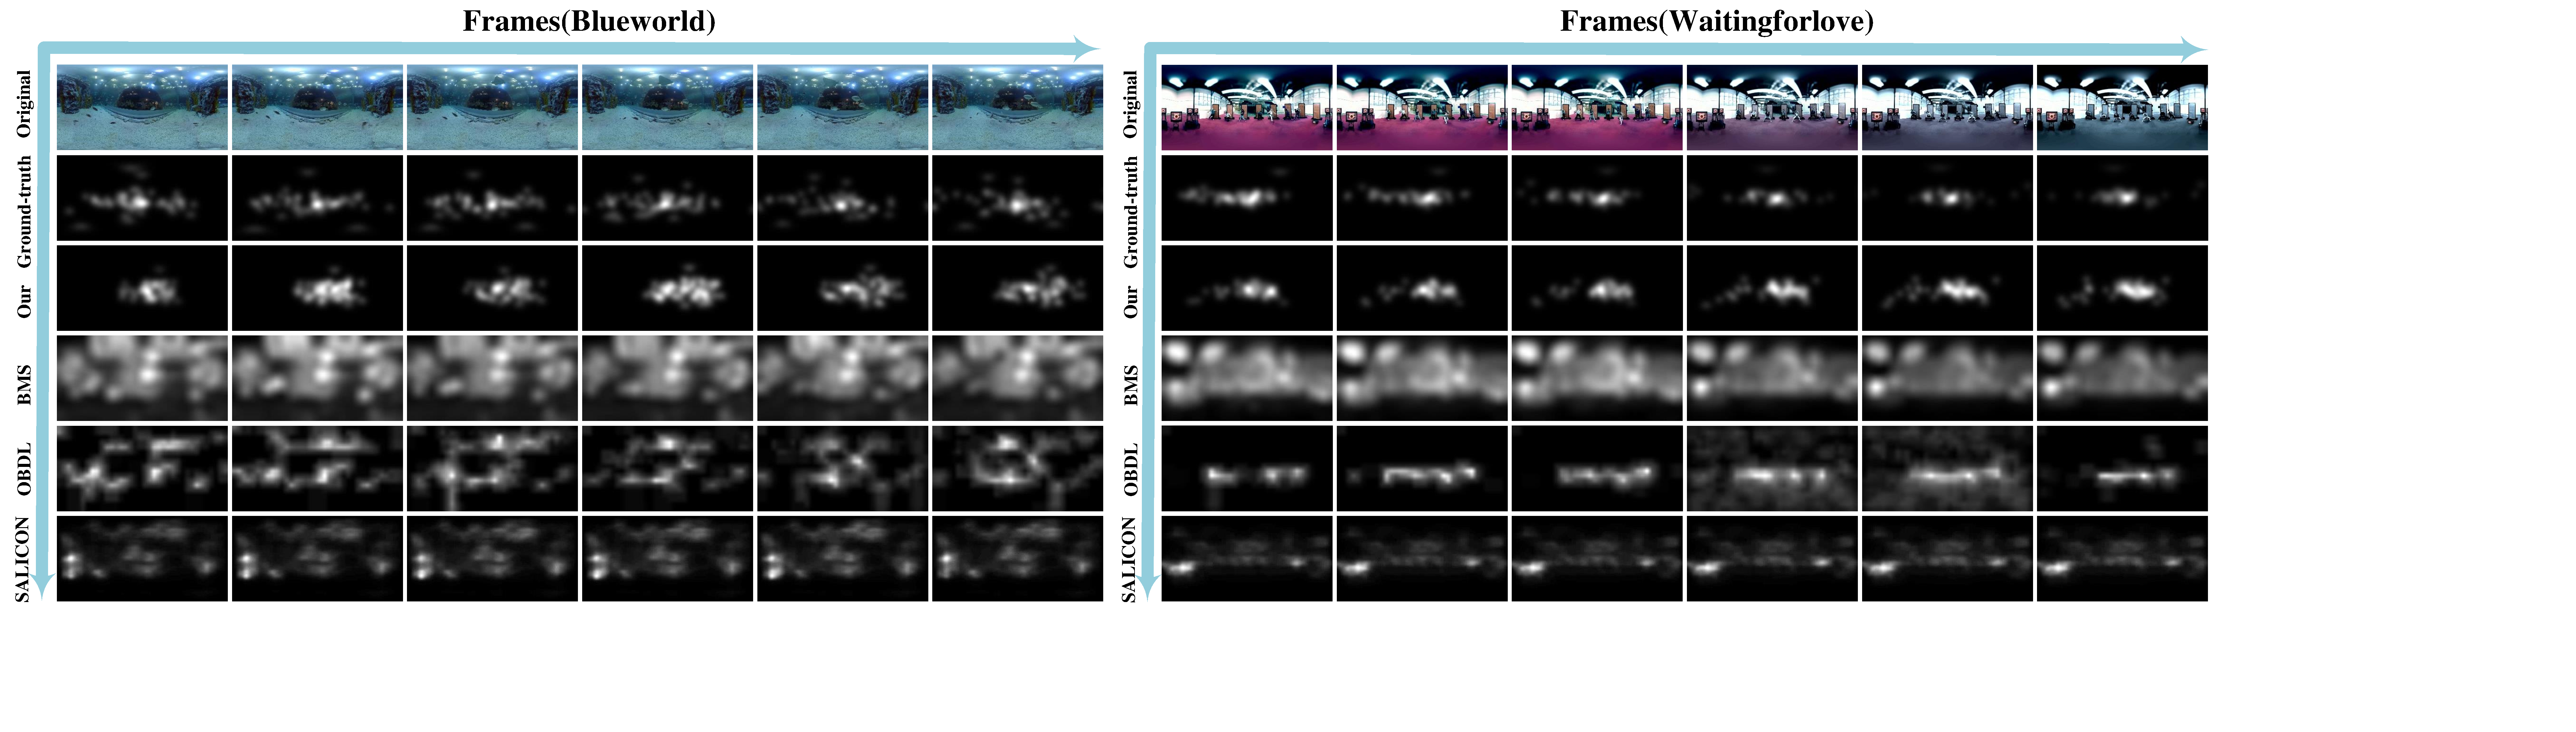
\includegraphics[width=2\columnwidth]{figures/experiment/objective_result_1}}%of
\vspace{-1em}
                  \caption{\footnotesize{HM maps of several frames selected from two test sequences in our PVS-HM database. They are all visualized in the 2D coordination.  The second row shows the ground-truth HM maps, which are generated upon the HM positions of all 58 subjects. The third to sixth rows show the HM maps of our, BMS \cite{zhang2016exploiting} , OBDL \cite{hossein2015many}, and SALICON \cite{huang2015salicon} approaches. }}
		\label{figure-object}
	\end{center}
\end{figure*}

\begin{table*}
\vspace{-.5em}
    \begin{center}
        \caption{MO results of online HM position prediction by our and other approaches.}
        \vspace{-1em}
        \label{table-result}
        \tiny
        \resizebox{\textwidth}{!}{
            \begin{tabular}{cc*{16}{c}c}

                            \tabincell{c}{\rotatebox{45}{Method}}
                                   & \rotatebox{45}{KingKong} & \rotatebox{45}{SpaceWar2} & \rotatebox{45}{StarryPolar} & \rotatebox{45}{Dancing} & \rotatebox{45}{Guitar}
                                   & \rotatebox{45}{BTSRun} & \rotatebox{45}{InsideCar} & \rotatebox{45}{RioOlympics} & \rotatebox{45}{SpaceWar} & \rotatebox{45}{CMLauncher2}
                                   & \rotatebox{45}{Waterfall} & \rotatebox{45}{Sunset} & \rotatebox{45}{BlueWorld} & \rotatebox{45}{Symphony} & \rotatebox{45}{WaitingForLove} & \rotatebox{45}{{\textbf{Average}}}

                \\
               \toprule
               \multirow{1}{*}{\rotatebox{0}{Online}}
               \abovespace

                           & \bf{0.809} & \bf{0.763} & \bf{0.549} & \bf{0.859} & \bf{0.785} & \bf{0.878} & \bf{0.847} & \bf{0.820} & \bf{0.626} & \bf{0.763} & \bf{0.667} & \bf{0.659} & \bf{0.693} & 0.747 & \bf{0.836} & \bf{0.753}
                         \\
                \multirow{1}{*}{\rotatebox{0}{Deep 360 Polit}}
                           & 0.340 & 0.208 & 0.322 & 0.537 & 0.541 & 0.615 & 0.206 & 0.270 & 0.391 & 0.205 & 0.082 & 0.464 & 0.352 & \bf{0.932} & 0.518 & 0.399
                         \\
                 \multirow{1}{*}{\rotatebox{0}{Baseline 1}}
                          & 0.201 & 0.206 & 0.161 & 0.216 & 0.203 & 0.206 & 0.216 & 0.203 & 0.209 & 0.205 & 0.203 & 0.204 & 0.206 & 0.202 & 0.211 & 0.204
                         \\
                         \belowspace
                 \multirow{1}{*}{\rotatebox{0}{Baseline 2}}
                          & 0.224 & 0.231 & 0.197 & 0.217 & 0.227 & 0.237 & 0.234 & 0.225 & 0.216 & 0.251 & 0.251 & 0.209 & 0.229 & 0.216 & 0.225 & 0.226
                         \\
                \bottomrule
            \end{tabular}
        }
    \end{center}
    \vspace{-1em}
\end{table*}

\subsection{Performance evaluation on offline-DHP}\label{sec:evaluation_offline}
\label{compare}



%\begin{figure*}
%\vspace{-1em}
%	\begin{center}
%		\centerline{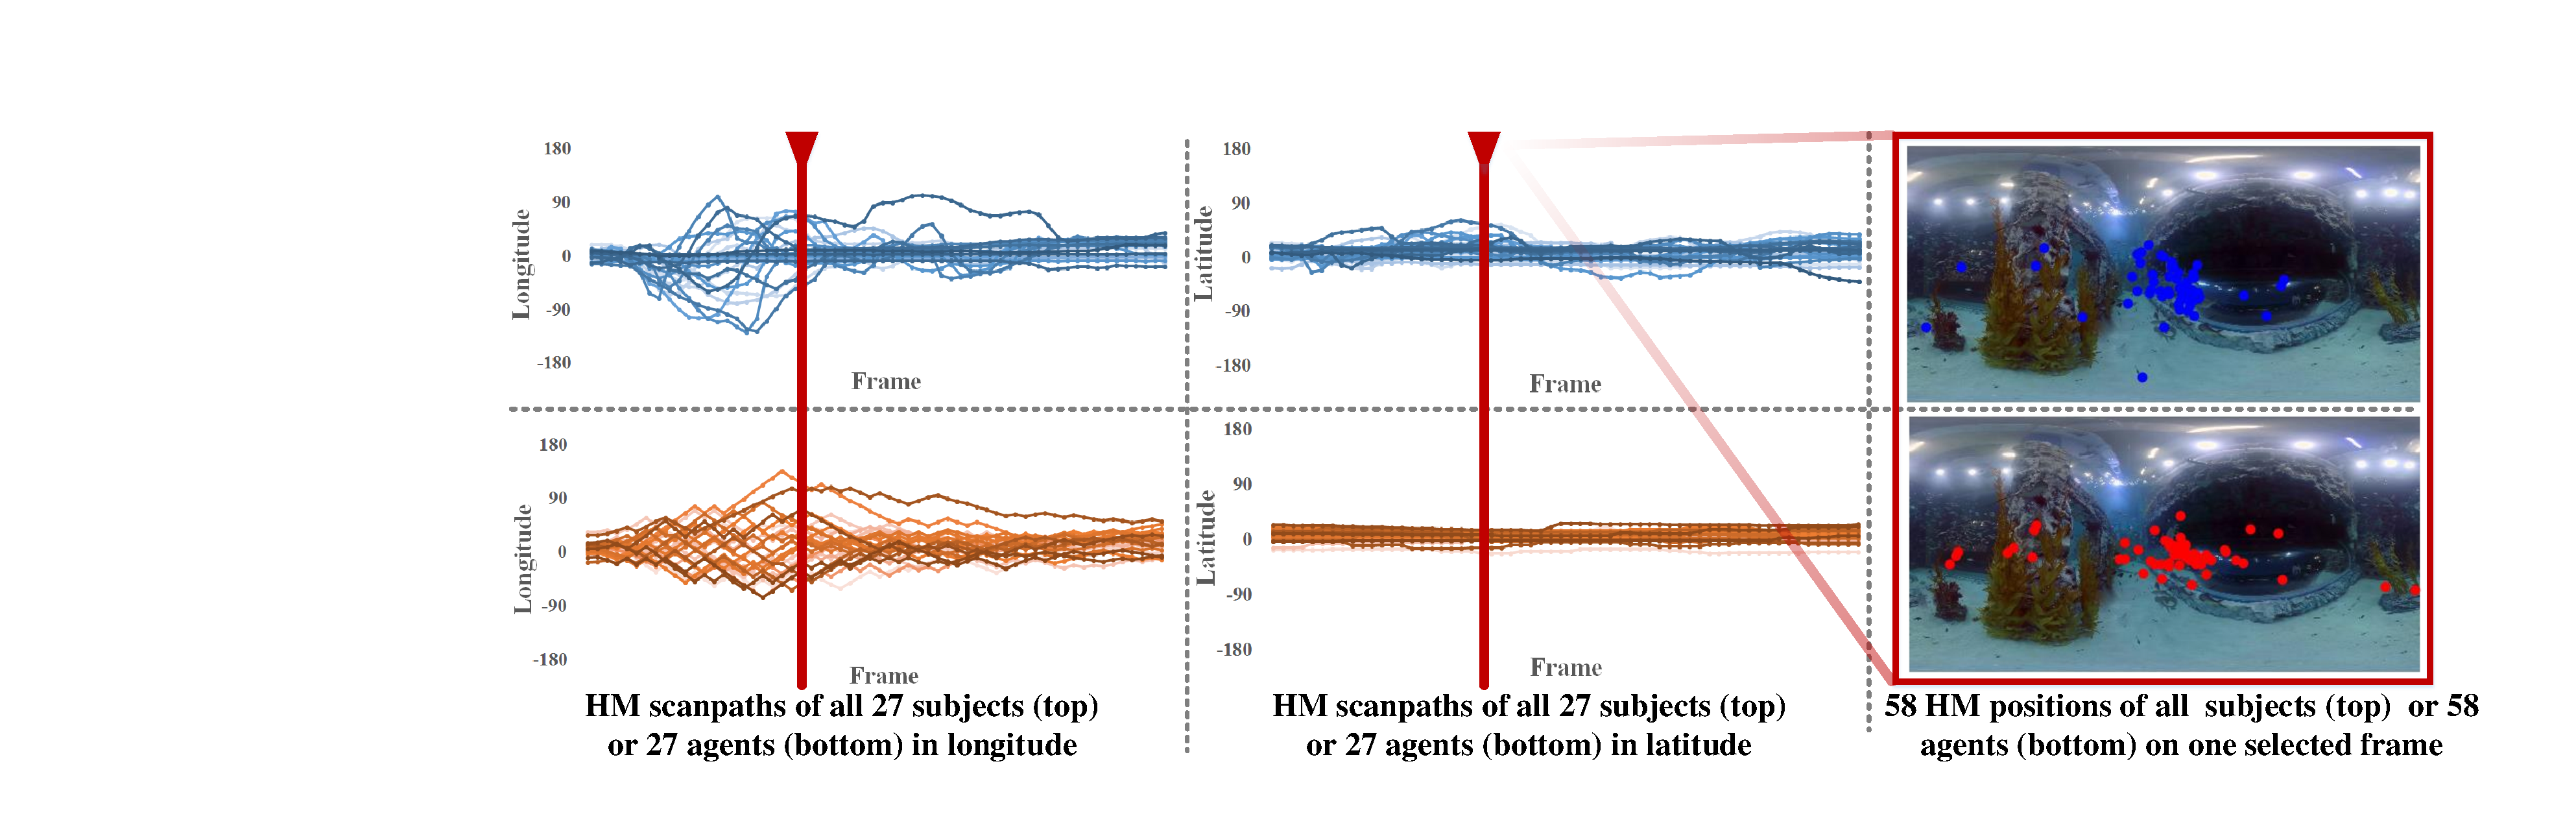
\includegraphics[width=1.5\columnwidth]{figures/experiment/scanpath_objective_result}}%of
%\vspace{-.5em}
%                   \caption{\footnotesize{XXX Visualization in scanpaths and positions of HM generated by ground-truth and our offline-DHP approach, for sequence \textit{BlueWorld}. The first and second columns show scanpaths of all the subjects (top) and DRL workflows (bottom), in longitude and latitude directions. The last column visualizes all HM positions of ground-truth (top) and our approach (bottom).}}
%		\label{scan-path-example}
%	\end{center}
%\vspace{-2em}
%\end{figure*}

Now, we evaluate the performance of our offline-DHP approach in predicting the HM maps of all 15 test sequences from the PVS-HM database. To the best of our knowledge, there is no work on predicting the HM maps of panoramic video, and saliency prediction is the closest field. Therefore, we compare our offline-DHP approach to three state-of-the-art saliency detection approaches: OBDL  \cite{hossein2015many}, BMS \cite{zhang2016exploiting} and SALICON \cite{huang2015salicon}.
In particular, OBDL  \cite{hossein2015many} and BMS \cite{zhang2016exploiting} are the latest saliency detection approaches for videos and images, respectively.
SALICON\cite{huang2015salicon} is a state-of-the-art DNN approach for saliency detection.
In addition to the above three approaches, we also compare our approach to the FCB baseline, since \textit{Finding 1} argues that human attention normally biases toward the front-center regions of panoramic video.
Here, we model FCB using a 2D Gaussian distribution, similar to the center bias of saliency detection.
Appendix A presents the details of the FCB modeling.
In the field of saliency detection, the center bias  \cite{borji2013state} is normally combined with saliency maps to improve the saliency detection accuracy. Hence, we further report the results of HM maps combined with the FCB feature, for our and other approaches.
See Appendix A for more details about the combination of FCB.
During the evaluation, we measure the prediction accuracy of HM maps in terms of CC and normalized scanpath saliency (NSS), which are two effective evaluation metrics \textcolor{blue}{\cite{Li_2015_ICCV}} in saliency detection.
Note that larger values of CC and NSS correspond to a more accurate prediction of HM maps.

Table \ref{table-result} tabulates the results of CC and NSS in predicting the HM maps of 15 test sequences, for our and other approaches.
In this table, the results of CC and NSS are averaged over all frames for each test sequence.
As shown in this table, when FCB is not integrated, our offline-DHP approach performs best among all four approaches and the FCB baseline, in terms of CC and NSS.
More importantly, once integrated with FCB, all four approaches have performance improvement, and our approach still performs considerably better than other approaches.
Specifically, our offline-DHP approach increases the average CC value by 0.198, 0.242 and 0.184, compared with OBDL, BMS and SALICON, respectively.
Additionally, the increase of average NSS value is 1.087, 1.245 and 1.001 in our approach, in comparison with OBDL, BMS and SALICON.
In a word, our offline-DHP approach is effective in predicting the HM maps of panoramic video, much better than other approaches and the FCB baseline.

%increases the CC value (averaged over all 15 test sequences) by 0.522, 0.412 and 0.479, compared with OBDL, BMS and SALICON, respectively.
%Additionally, the increase of averaged NSS value is 2.709, 2.230 and 2.497 in offline-DHP, over OBDL, BMS and SALICON.
%Once integrated with FCB, all four approaches have performance improvement, and our approach still performs best among all three approaches. Meanwhile, our approach significantly outperforms the FCB baseline.



Next, we compare the subjective results. Figure \ref{figure-object} shows several frames from two selected sequences and their ground-truth HM maps.
In Figure \ref{figure-object}, we further visualize the HM maps generated by our and other approaches. Here, the predicted HM maps are integrated with FCB, since the FCB feature can improve the performance of all four approaches (as presented in Table \ref{table-result}).
From this figure, one can observe that the HM maps of our approach are considerably closer to the ground-truth HM maps, compared with the other approaches.
This result indicates that our offline-DHP approach is capable of better locating the HM positions of different subjects on panoramic video.
%Moreover, for one selected video frame, Figure \ref{scan-path-example} plots the HM scanpaths by all subjects and by all DRL workflows of offline-DHP, to investigate the agreement between the subjects and DRL workflows.
%As shown in this figure, the DRL workflows are able to obtain similar scanpaths as humans.  Figure \ref{scan-path-example} further shows all HM positions of the selected frame, which are obtained from the ground-truth and predicted HM scanpaths. As seen in this figure, the HM positions can be well predicted by our offline-DHP approach. In conclusion, our offline-DHP approach is effective in modeling HM maps by predicting both scanpaths and positions of HM for panoramic video.




%Iceclear online

\subsection{Performance evaluation on online-DHP}\label{sec:evaluation_online}
\label{online-compare}

%\begin{table*}
%	\begin{center}
%		\caption{MO results of HM position prediction by our and other approaches} \centerline{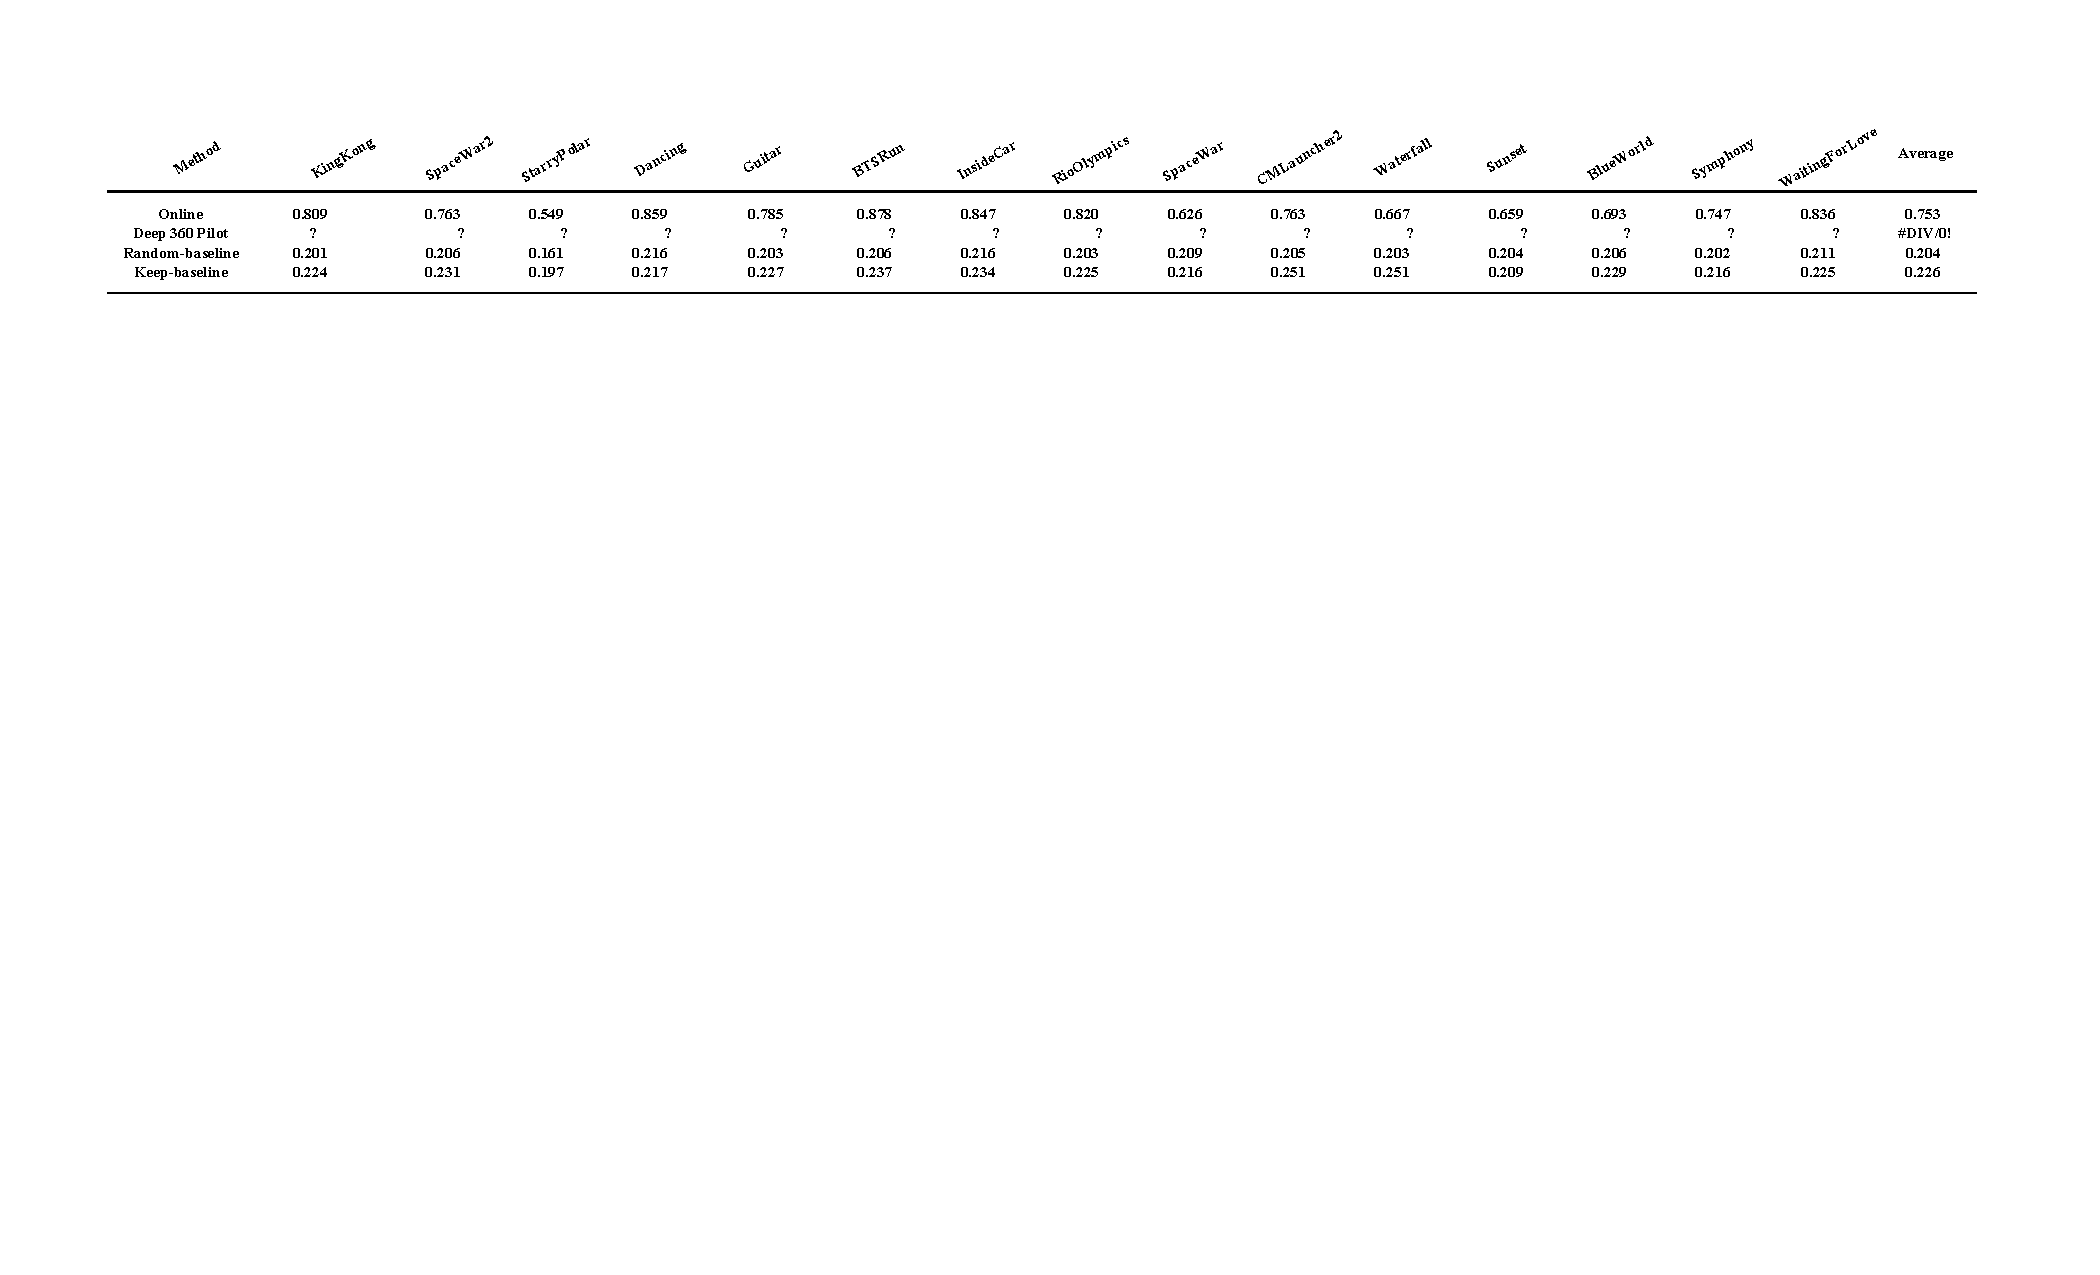
\includegraphics[width=2\columnwidth]{figures/experiment_on_line/Online_compare}}%of
%		\label{table-MeanMo}
%	\end{center}
%\end{table*}

% the Ice Table


This section evaluates the performance of our online-DHP approach for predicting HM positions in the online scenario.
The online scenario refers to predicting the HM position of one subject at each panoramic frame based on the observed HM positions of this subject at the previous frames.
In our experiments, we compare the performance of online-DHP with the state-of-the-art deep 360 pilot \cite{hu2017deep}, which is the only existing approach for the online prediction of HM positions in panoramic video.
We also compare our online-DHP approach with two baselines. According to \textit{Finding 6}, the first baseline (called baseline 1) keeps the HM scanpath of the current frame the same as that at the previous frame, such that the online HM position at each frame can be generated.
The second baseline (called baseline 2) produces the HM positions, using the randomly generated HM scanpaths. The same as \cite{hu2017deep}, MO of \eqref{mo-defination} is measured as the metric to evaluate the accuracy of online prediction in HM positions. Note that a larger value of MO means a more accurate online prediction in HM positions.
%The performance evaluation is conducted on the test set of our PVS-HM database.
%More specifically, the HM positions of 58 subjects on the 15 test sequences of the PVS-HM are all tested.



\begin{figure*}
\vspace{-1em}
	\begin{center}
		\centerline{\subfigure[Dancing]{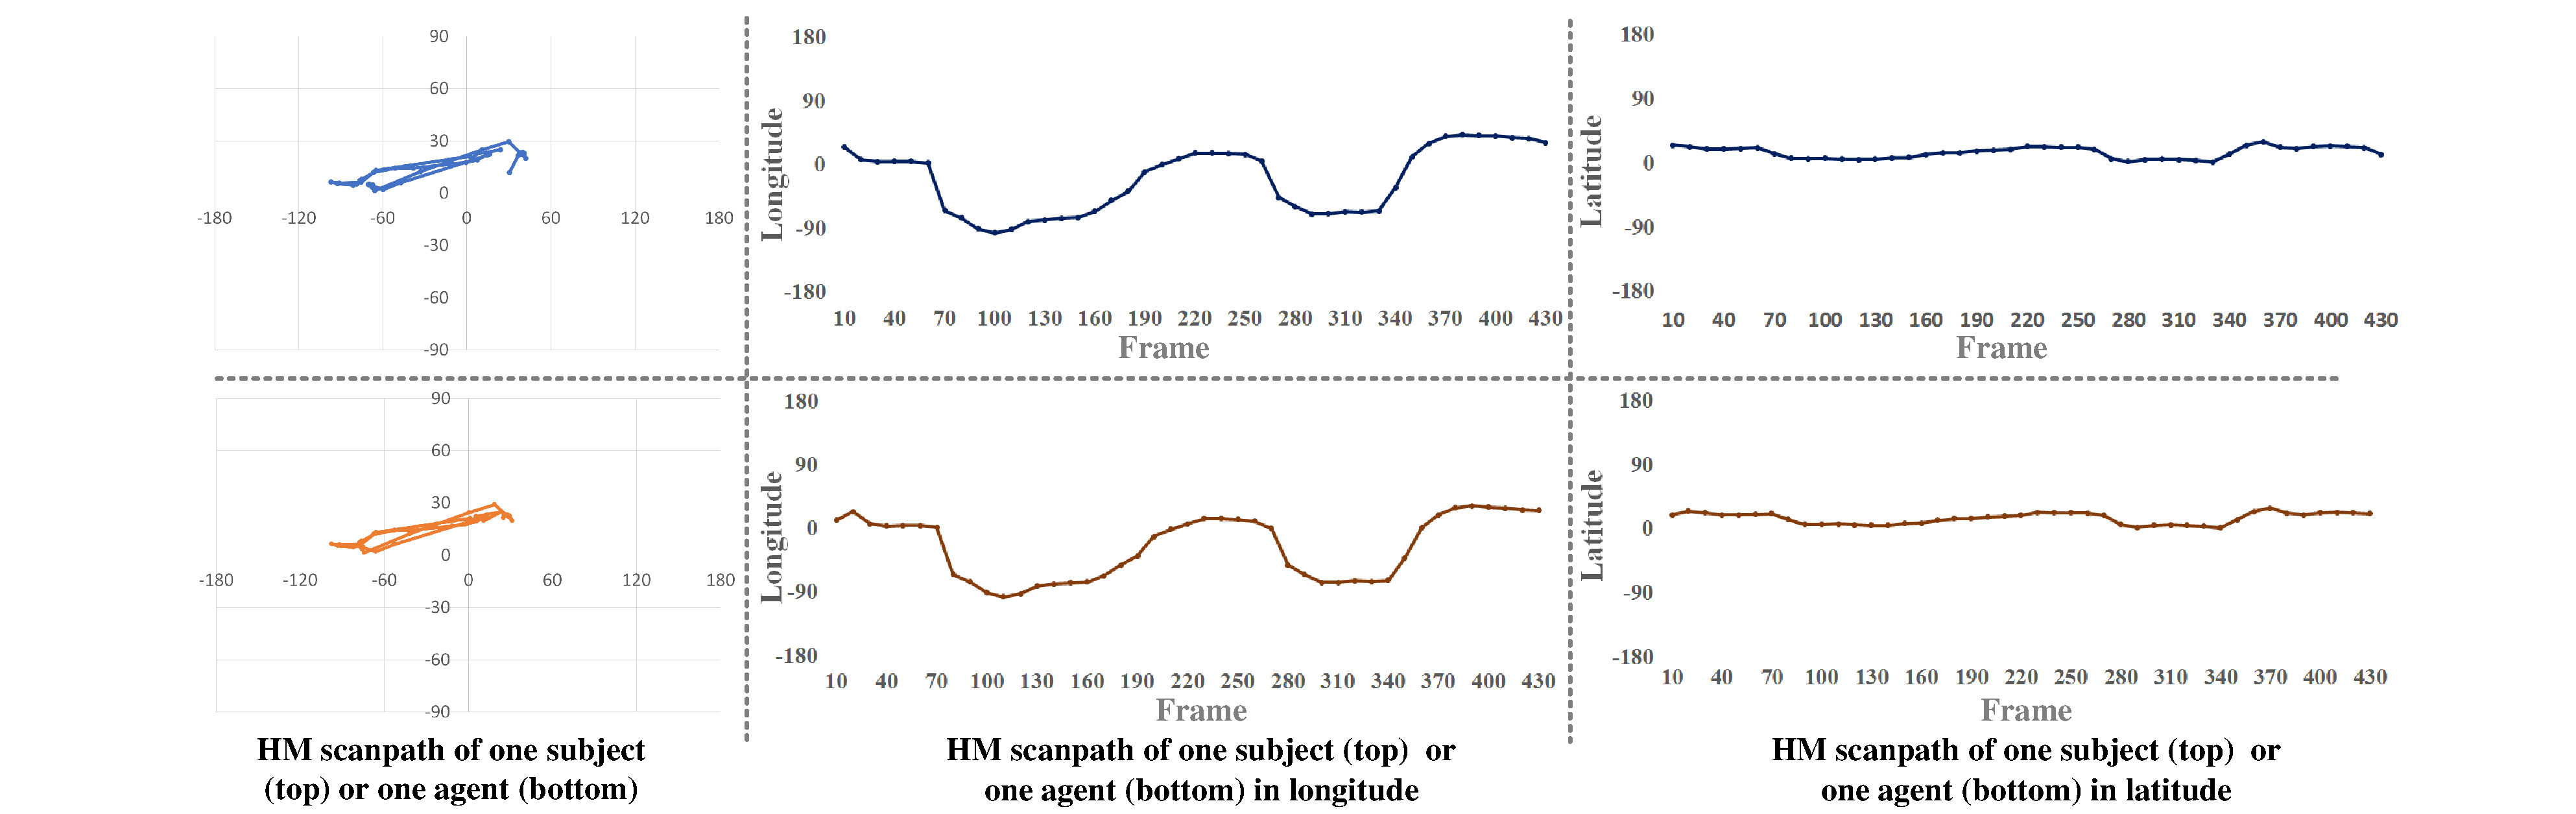
\includegraphics[width=1.5\columnwidth]{figures/experiment_on_line/scanpath_Dancing}}}%of
\vspace{-1em}
        \centerline{\subfigure[KingKong]{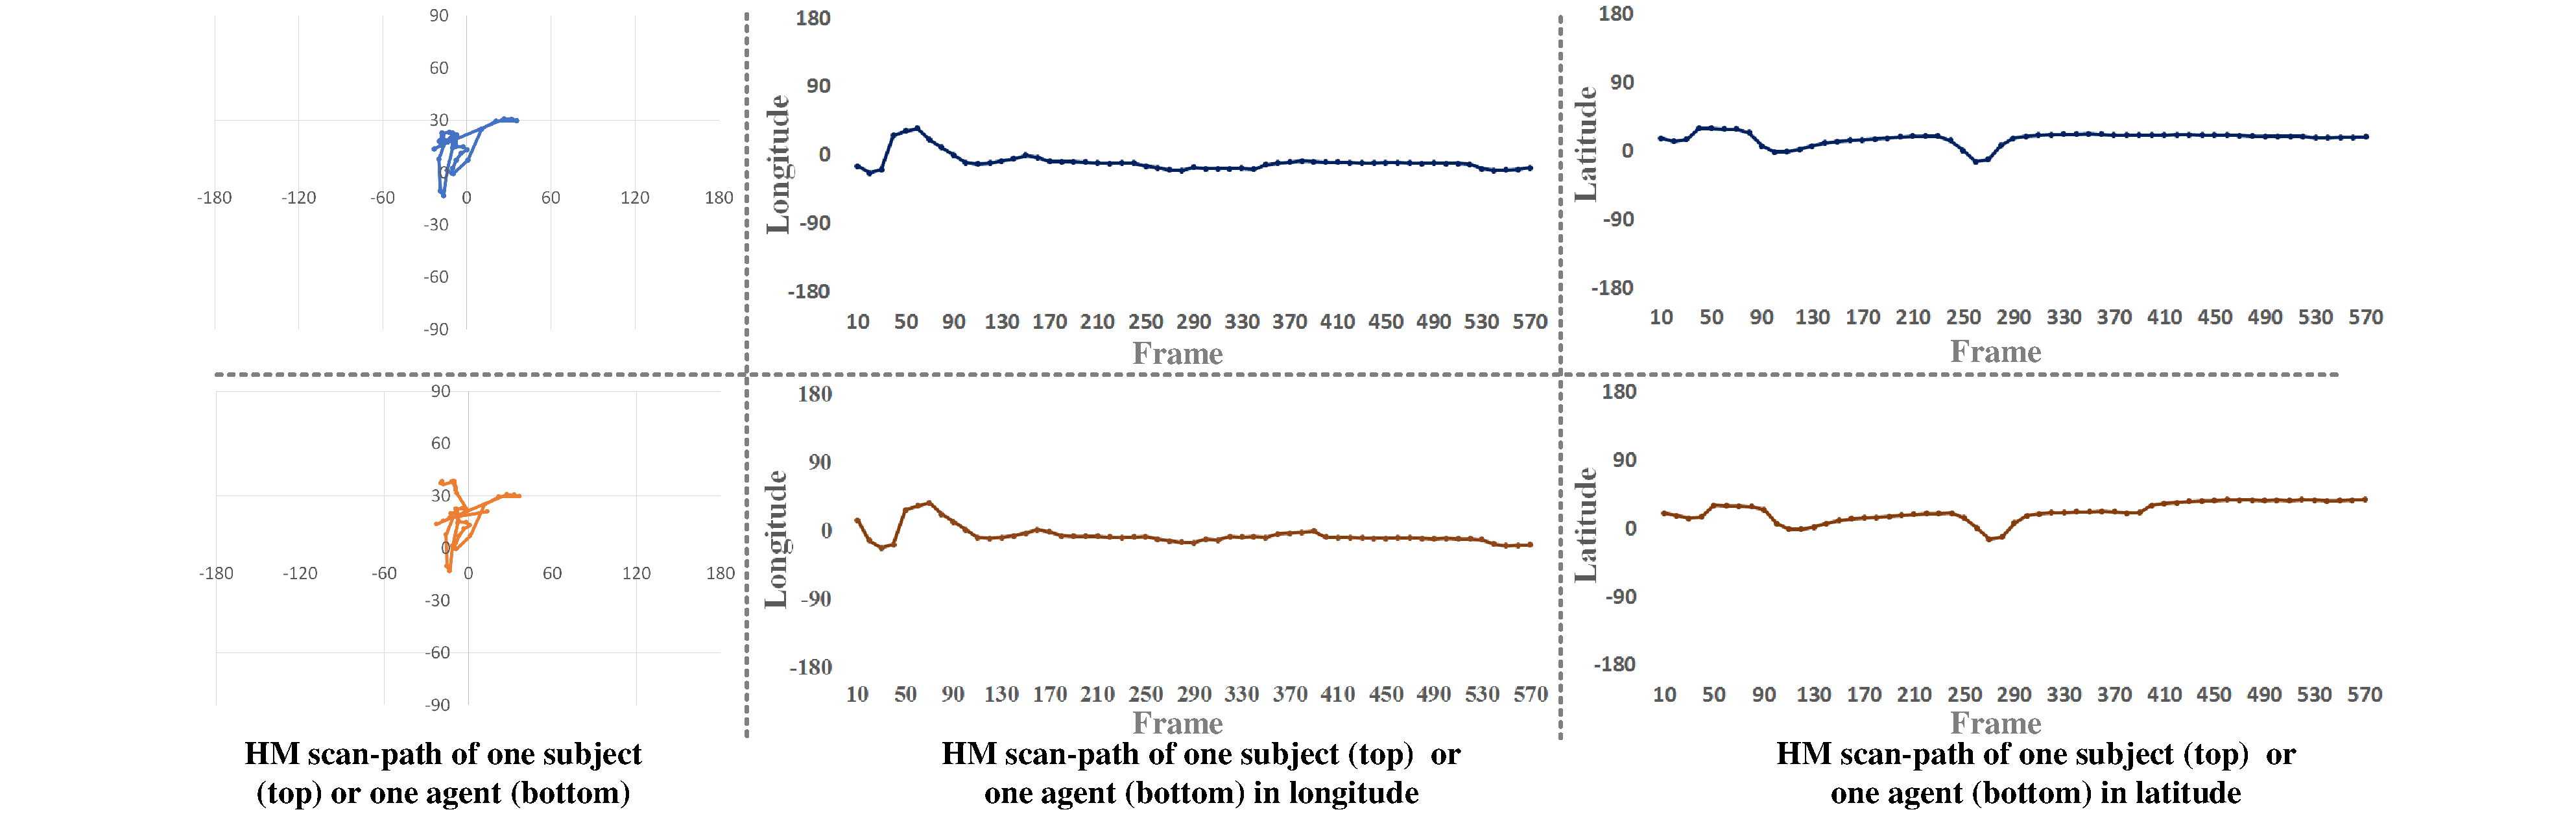
\includegraphics[width=1.5\columnwidth]{figures/experiment_on_line/scanpath_Kingkong}}}%of
\vspace{-1em}
                   \caption{\footnotesize{Visualization in HM scanpaths generated by one subject and the online-DHP approach, for sequences \textit{Dancing} and \textit{KingKong}. Note that the HM scanpaths of one subject (among 58 subjects) are randomly selected and plotted, and then the corresponding HM scanpaths predicted by online-DHP are plotted.}}
		\label{scan-path-example}
	\end{center}
\vspace{-2em}
\end{figure*}

\begin{figure*}
	\begin{center}
		\centerline{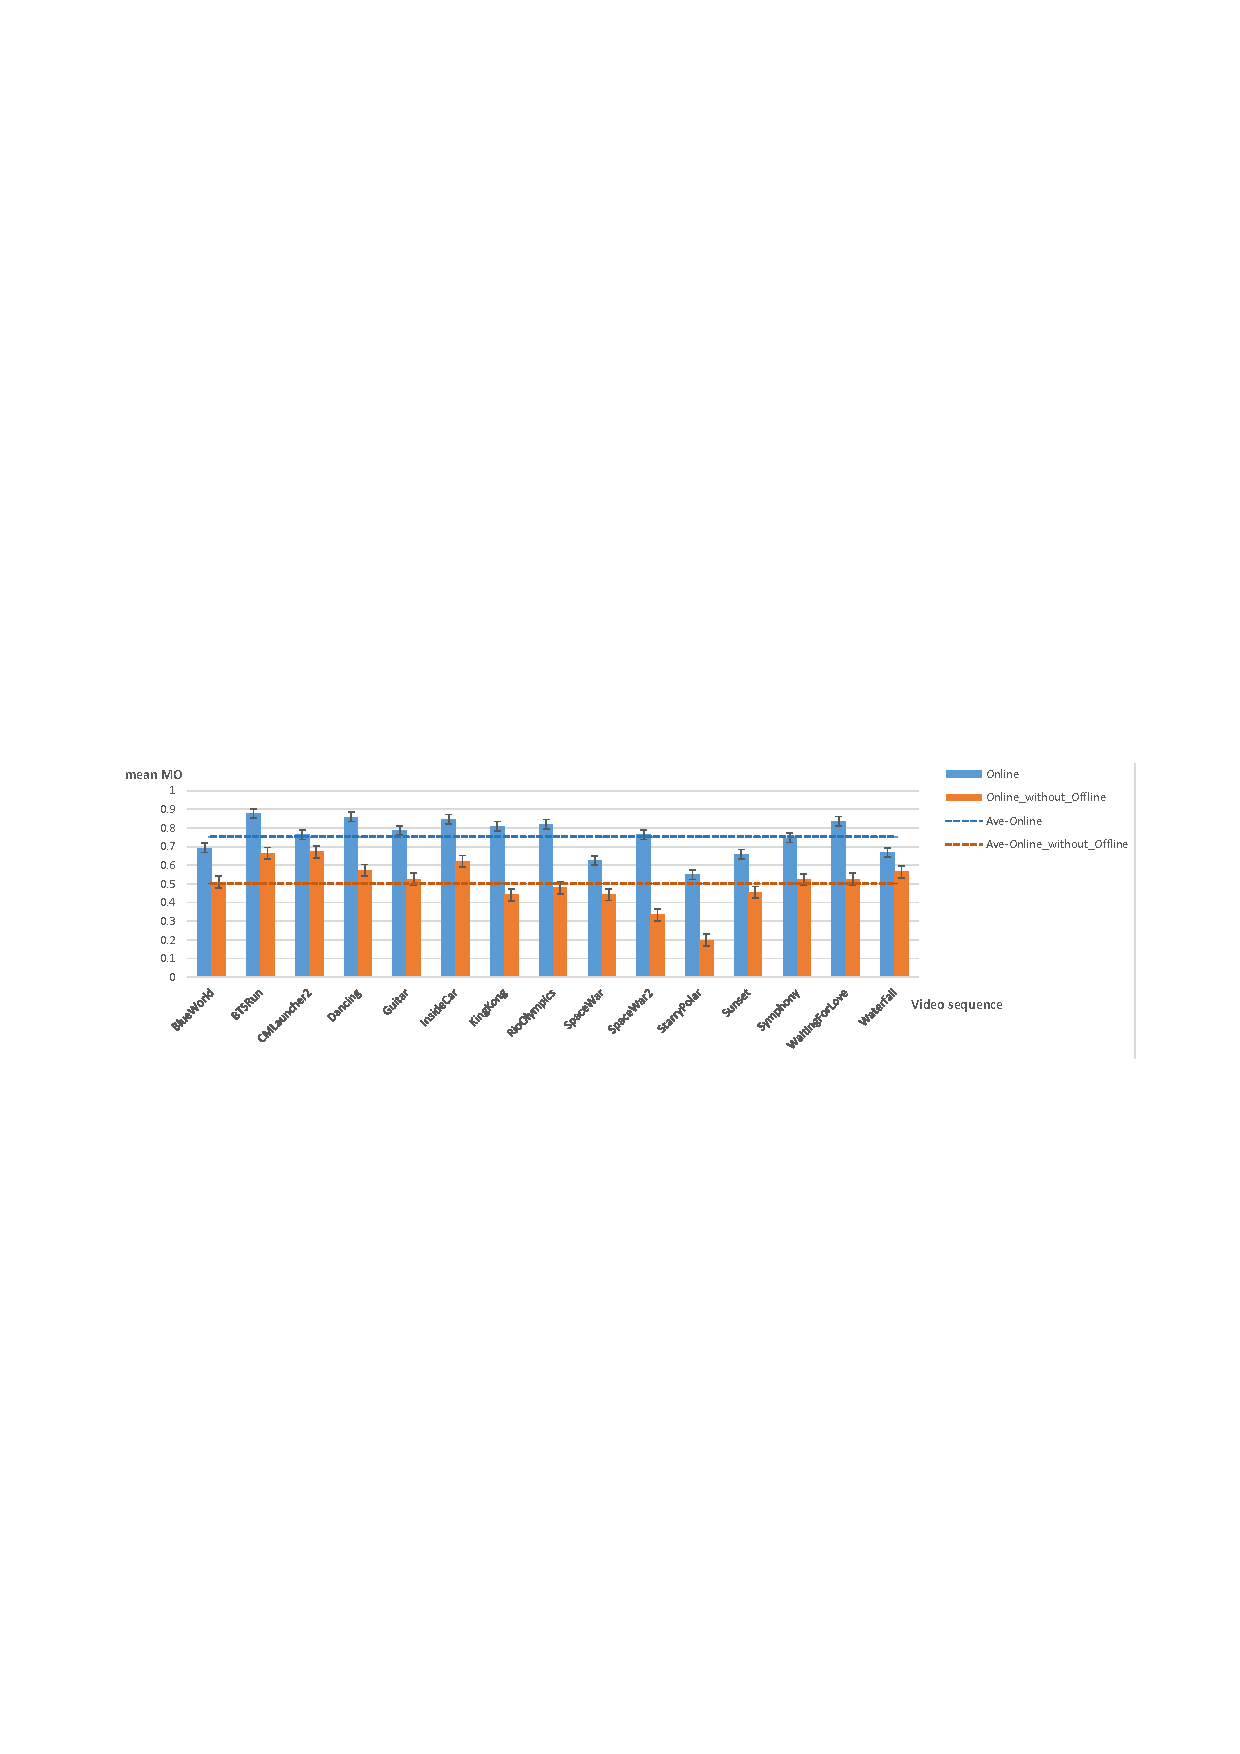
\includegraphics[width=2\columnwidth]{figures/experiment_on_line/Mean_MO}}%of
      \vspace{-2em}
		\caption{\footnotesize{MO results between the online-DHP approaches with and without the trained offline-DHP network.}}
		\label{Online_compare}
	\end{center}
\vspace{-2em}
\end{figure*}

Table \ref{table-result} compares the MO results of our and other approaches for the 15 test sequences of our PVS-HM database. Note that the MO results of each sequence are averaged over the predicted HM positions of all 58 subjects in our database. As observed in this table, our online-DHP approach is significantly superior to two baselines, indicating the effectiveness of applying DRL to predict HM positions online.
Table \ref{table-result} also shows that our online-DHP approach performs considerably better than the deep 360 pilot \cite{hu2017deep}, with an increase of 0.354 in average MO.
In addition, as shown in Table \ref{table-result}, our approach outperforms \cite{hu2017deep} over almost all sequences.
The performance improvement of our approach is probably because (1) the online DRL model of our approach is capable of generating the accurate \textit{actions} of HM scanpaths, and (2) the DRL network of offline-DHP is incorporated in our online prediction as the prior knowledge. Moreover, our approach is also effective for the generic panoramic sequences, while \cite{hu2017deep} fails in scenery panoramic video. For example, the MO result of \cite{hu2017deep} for the sequence Waterfall is $0.082$, which is far less than $0.667$ MO of online-DHP. This result is primarily because the deep 360 pilot \cite{hu2017deep} relies heavily on the object detection of RCNN.

Moreover, we visualize the ground-truth and predicted HM scan-paths, for subjective evaluation.
Specifically, Figure \ref{scan-path-example} plots the HM scanpaths by one subject and by the online-DHP approach, for the panoramic sequences of Dancing and KingKong.
As shown in this figure, online-DHP is able to obtain similar scanpaths as the subject, such that the HM positions can be accurately predicted online for each panoramic frame.
In conclusion, our subjective evaluation, together with the above objective MO comparison, illustrates that the proposed online-DHP approach is effective in predicting the HM positions with the online manner.

%Moreover, for one selected video frame, Figure \ref{scan-path-example} plots the HM scanpaths by all subjects and by all DRL workflows of offline-DHP, to investigate the agreement between the subjects and DRL workflows.
%As shown in this figure, the DRL workflows are able to obtain similar scanpaths as humans.  Figure \ref{scan-path-example} further shows all HM positions of the selected frame, which are obtained from the ground-truth and predicted HM scanpaths. As seen in this figure, the HM positions can be well predicted by our offline-DHP approach. In conclusion, our offline-DHP approach is effective in modeling HM maps by predicting both scanpaths and positions of HM for panoramic video.

To test the generalizability of our approach, we further evaluate the performance of our, the deep 360 pilot \cite{hu2017deep} and the two baseline approaches on the  sports-360 dataset of \cite{hu2017deep}. For this evaluation, our online-DHP is still based on our offline DRL network that is learned from the training sequences of our PVS-HM database. The MO results are presented in Table \ref{table-result-on360}. From this table, one may observe that our online-DHP approach again outperforms \cite{hu2017deep} and the two baselines, despite testing on the test set of \cite{hu2017deep}. In particular, the MO result of our approach is 0.90  for the panoramic sequences of dance, with 0.11 MO increase over \cite{hu2017deep}. Additionally, our approach improves the MO results of \cite{hu2017deep} by 0.07, 0.01, 0.01, and 0.10, for the sequences of skateboarding, parkour, BMX and basketball, respectively. In other words, the online-DHP approach is superior to the state-of-the-art approach \cite{hu2017deep} in the online prediction of HM positions, over almost all classes of panoramic video sequences.  Therefore, the generalization capability of our online-DHP approach can be confirmed.

It is interesting to analyze the benefits of incorporating the DRL network of offline-DHP in our online-DHP approach, since the online-DHP approach is based on the offline DRL network. Figure \ref{Online_compare} shows the MO results of our online-DHP approach with and without the offline DRL network. As observed in this figure, the offline DRL network is able to increase the MO results of our online-DHP approach, for all 15 sequences. In addition, the MO value can be increased from 0.502 to 0.753 on average, when the offline DRL network is incorporated in online-DHP. Therefore, the learned DRL network of offline-DHL also benefits the online prediction of HM positions in online-DHL.

%In online-DHP, the performance of online HM prediction is related to the hyperparameters of $th_{\text{MO}}$, XXX, and XXX. In the following, we analyze the influences of this hyperparameters on the performance of online-DHP. Figure XXX shows the MO results at various values of $th_{\text{MO}}$, XXX, and XXX. The hyperparameter $th_{\text{MO}}$ is the threshold of the MO value achieved by XXX, and it determines whether the \textit{action} of online-DHP is output as the HM scanpath at the current frame. We can see from Figure XXX that XXX is increased at $th_{\text{MO}}\in XXX$ and converged once $th_{\text{MO}}\geq???$. Thus, in this paper, we set $th_{\text{MO}}$ to be XXX.

%\textcolor{blue}{Now, we move to the evaluation of Online-DHP. We compare our Online-DHP approach with Deep 360 Pilot approach\cite{hu2017deep} and two baselines.}
%
%\textcolor{blue}{Table \ref{table-MeanMo} compares mean MO results of our and other approaches, in predicting HM positions over all 15 test sequences of panoramic video.
%Here, MO results are averaged over all frames for each test sequence.
%The Random-baseline means predicting the HM position in a totally random way.
%And the Keep-baseline means predicting the HM position due to the HM position of the former frame.
%We can see from this table that our approach performs far better than other approaches. Specifically, our approach has ? average increment over Deep 360 Pilot approach\cite{hu2017deep}.
%We think that is mostly because that our approach has priori knowledge from the Offline-DHP.
%For the two baselines, the Keep-baseline is a little better than the Random-baseline mostly because of the guidance of the former frame.
%Compared with the two baselines, our approach is also obviously much more effective.}
%
%\textcolor{blue}{Offline-DHP is an important component of our approach.
%Figure \ref{Online_compare} shows the result of mean MO between Online-DHP and Online-DHP without Offline-DHP.
%We can see that the Offline-DHP enhances the performance of online prediction a lot.
%We think it's mostly because the Offline-DHP provides priori knowledge for the online prediction.
%And this is very effective in predicting.}
%
%\textcolor{blue}{After the comparison, we move to the analysis of an important parameter $th_{MO}$ in algorithm \ref{online-DHP-algorithm}, which affects both the result of MO\eqref{mo-defination} and the time complexity of our approach.
%We call it the threshold of MO.
%According to our approach, we think the threshold $th_{MO}$ is positively correlated with the result of MO, but negatively correlated with the time complexity.}
\begin{table}
	\vspace{-.5em}
	\begin{center}
		\caption{MO results for online prediction of HM positions over the sports-360 dataset.}
		\vspace{-1em}
		\label{table-result-on360}
		\tiny
		\resizebox{.47\textwidth}{!}{
			\begin{tabular}{c c c c c c}
				
				Method
				& Skateboarding & Parkour & BMX & Dance & Basketball
			
				\\
				\toprule
				DHP
				\abovespace
				
				& \bf{0.78} & \bf{0.75} & \bf{0.72} & \bf{0.90} & \bf{0.77}
				\\
				Deep 360 Polit
				& 0.71 & 0.74 & 0.71 & 0.79 & 0.67
				\\
				Baseline 1
				& 0.15 & 0.17 & 0.16 & 0.17 & 0.17
				\\
				
				Baseline 2
				& 0.22 & 0.19 & 0.18 & 0.22 & 0.18
				\\
				\bottomrule
			\end{tabular}
		}
	\end{center}
	\vspace{-1em}
\end{table}






\section{Conclusion}
In this paper, we have proposed the DHP approach for predicting HM positions on panoramic video. First, we established a new database named PVS-HM, which includes the HM data of 58 subjects viewing 76 panoramic sequences. We found from our database that the HM positions are highly consistent across humans. Thus, the consistent HM positions on each panoramic frame can be represented in the form of an HM map, which encodes the possibility of each pixel being the HM position. Second, we proposed the offline-DHP approach to estimate HM maps in an offline manner. Specifically, our offline-DHP approach leverages DRL to make decisions on \textit {actions} of HM scanpaths, via optimizing the \textit{reward} of imitating the way of humans view panoramic video.
Subsequently, the HM scanpaths of several \textit{agents} from multiple DRL workflows are integrated to obtain the final HM maps.
Third, we proposed the online-DHP approach, which predicts the HM positions of one subject online. In online-DHP, the DRL algorithm was developed to determine the HM positions of one \textit{agent} at the incoming frames, given the \textit{observation} of previous HM scanpaths and the current video content. The DRL algorithm is based on the learned model of offline-DHP in extracting the spatio-temporal features of attention-related content. Finally, the experimental results showed that both offline-DHP and online-DHP are superior to other conventional approaches, in the offline and online tasks of HM prediction for panoramic video.

Humans always perceive the world around them in a panorama, rather than a 2D plane. Therefore, modeling attention on panoramic video is an important component in establishing human-like computer vision systems. Our work at the current stage mainly focuses on predicting HM positions, as the first step toward attention modeling of panoramic video. Future work should further predict eye fixations within FoV regions of panoramic video. The potential applications of our approach are another promising work in future. For example, the online-DHP approach may be embedded in robotics, to mimic the way in which humans perceive the real world. Besides, panoramic video has large perceptual redundancy, since most of the panoramic regions cannot be seen by humans. It is thus possible to use the offline-DHP approach to remove such perceptual redundancy, such that the bit-rates of panoramic video coding can be dramatically saved.





% if have a single appendix:
%\appendix[Proof of the Zonklar Equations]
% or
%\appendix  % for no appendix heading
% do not use \section anymore after \appendix, only \section*
% is possibly needed

% use appendices with more than one appendix
% then use \section to start each appendix
% you must declare a \section before using any
% \subsection or using \label (\appendices by itself
% starts a section numbered zero.)
%


\appendices
\section{Analysis of FCB Combined in HM Maps}

The saliency detection literature \cite{judd2009learning} has argued that human attention has strong center bias in images or videos, and that the incorporation of center bias can improve the performance of saliency detection. Similarly, FCB exists when viewing panoramic videos, as discussed in \textit{Finding 1}. Hence, this appendix presents the combination of the FCB feature and the offline-DHP approach. Here, we apply the FCB feature as an additional channel in generating the HM maps of panoramic videos. Specifically, assume that $\mathbf{H}^f$ is the HM map generated by the channel of the FCB feature. Similar to the center bias feature of image saliency detection \cite{judd2009learning}, we apply the following 2D Gaussian distribution to model $\mathbf{H}^f$ at each frame:
\begin{equation}
\label{Gauss_sigma}
\mathbf{H}^f(u,v)= \exp\left({-\frac{(u-u_f)^2+(v-v_f)^2}{\sigma_f^2}}\right),
\end{equation}
where $(u,v)$ are the longitude and latitude of the GDS location in the map, and $(u_f,v_f)$ are the longitude and latitude of the front center position in GDS. In addition, $\sigma_f$ is the standard deviation of  the 2D Gaussian distribution.

Next, we need to combine $\mathbf{H}^f$ with the predicted HM map $\mathbf{H}_t$ by
\begin{equation}
\label{optmization_x}
\mathbf{H}^c_t = w_1\cdot \mathbf{H}^f+w_2\cdot \mathbf{H}_t,
\end{equation}
for each panoramic frame. In the above equation, $\mathbf{H}^c_t$ is the HM map integrated with the FCB feature for frame $t$; $w_1$ and $w_2$ are the weights corresponding to the channels of $\mathbf{H}_c$ and $\mathbf{H}_t$, respectively. Given \eqref{Gauss_sigma} and \eqref{optmization_x}, the following optimization formulation is applied to obtain the values of $\sigma_f$, $w_1$ and $w_2$:
\begin{equation}
\label{optmization_w}
\max_{\sigma_f,w_1,w_2} \sum_{t=1}^{T} \text{CC}(\mathbf{H}^c_t, \mathbf{H}^g_t), \quad \text{s.t.} \quad w_1+w_2=1.
\end{equation}
In \eqref{optmization_x}, $\mathbf{H}^g_t$ is the ground-truth HM map of each frame; $\text{CC}(\cdot,\cdot)$ indicates the CC value of two maps. Then, we solve the above optimization formulation by the least square fitting of CC over all training data of our PVS-HM database. Consequently, the optimal values of $\sigma_f$, $w_1$ and $w_2$ are $21.1^\circ$, $0.52$ and $0.48$, respectively. These values are used to integrate the FCB feature in our offline-FCB approach. Note that the same way is applied to obtain the weights of $w_1$ and $w_2$, when combining the FCB feature with other approaches.

Figure \ref{fitting_surface} shows the results of  CC between the predicted and ground-truth HM maps at various values of $\sigma_f$ and $w_1$. From this figure, we can see that the CC results vary from $0.44$ to $0.70$ alongside the increase of $w_1$ from $0$ to $1$, reaching the maximum value at $w_1=0.52$ given $\sigma_f=21.1^\circ$. This indicates that both the FCB feature and our offline-DHP approach are effective in predicting the HM maps of panoramic video, and that the effectiveness of the FCB feature is different at varying combination weights. In addition, as shown in Figure \ref{fitting_surface}, at $w_1=0.52$, the CC value increases from 0.66 to 0.70, when $\sigma_f$ grows from $7^\circ$ to $21.1^\circ$, and then it decreases to 0.63 until $\sigma_f = 43.6^\circ$. Thus, the standard deviation of the 2D Gaussian distribution in \eqref{Gauss_sigma} is set to be $21.1^\circ$ for the FCB feature in our experiments.


\begin{figure}
\vspace{-1em}
	\begin{center}
		\centerline{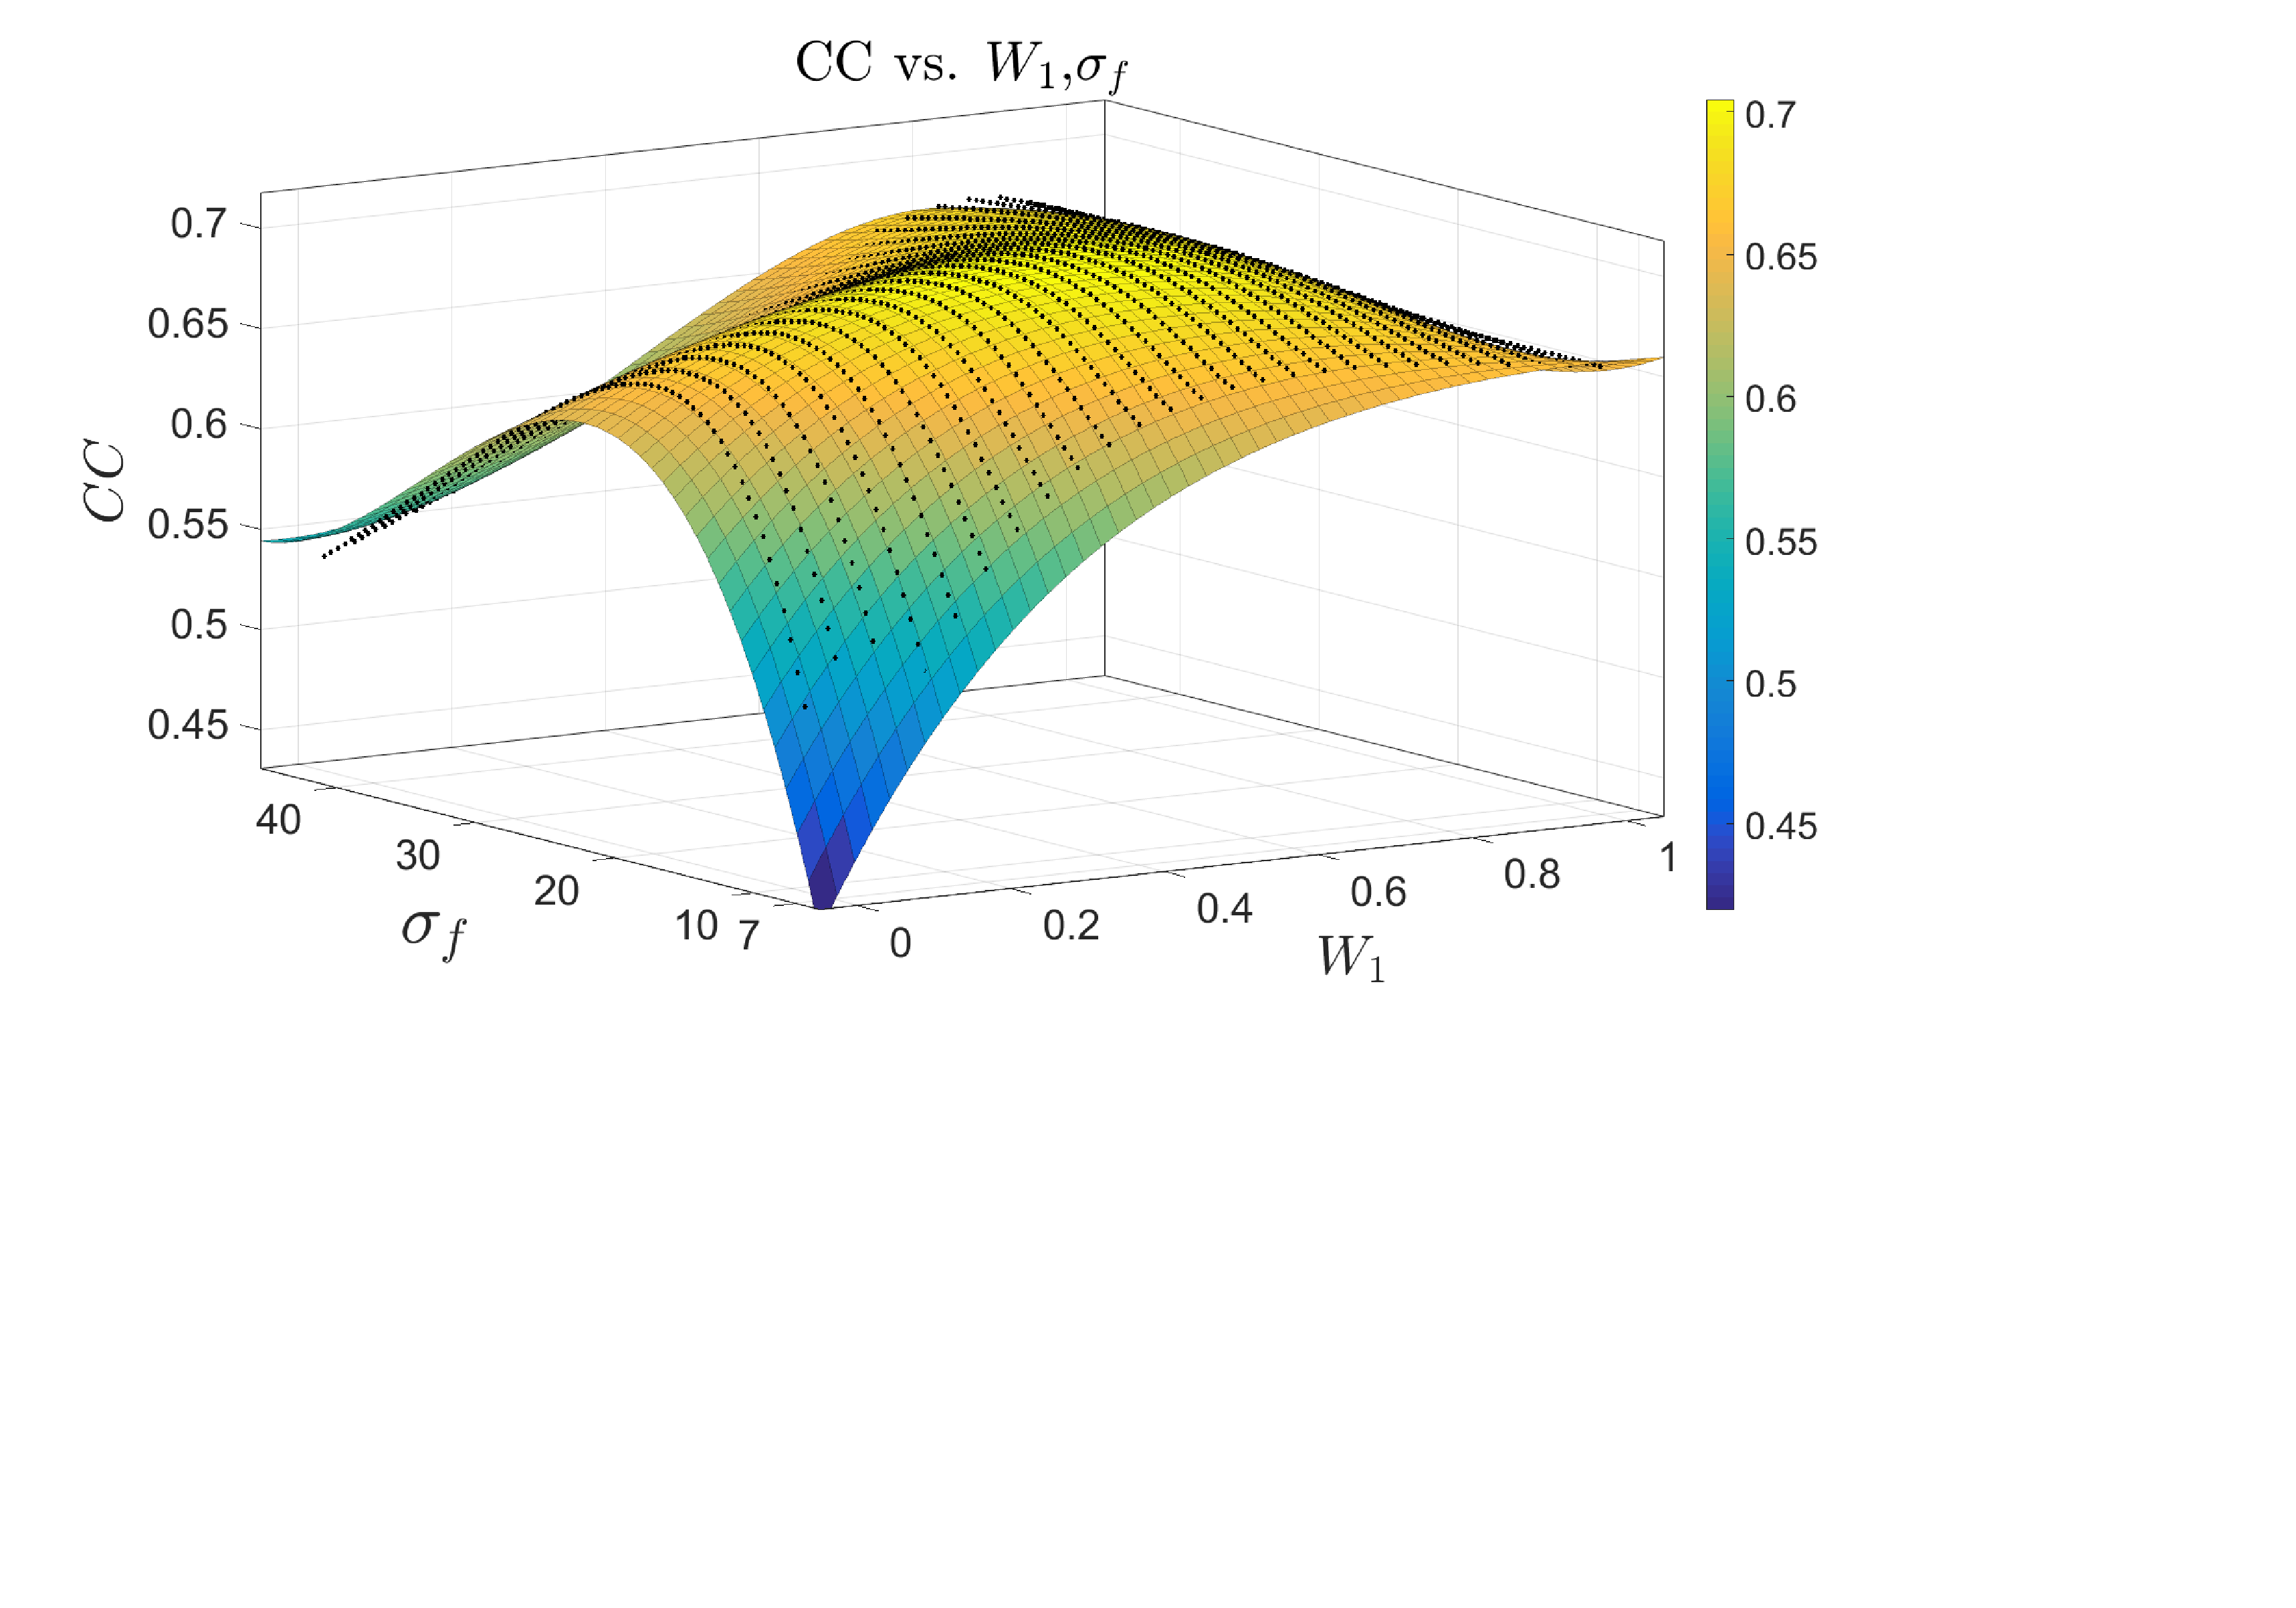
\includegraphics[width=.8\columnwidth]{figures/experiment/Fitting}}%of
      \vspace{-1em}
		\caption{\footnotesize{The fitting surface of CC results between the predicted and ground-truth HM maps at various $\sigma_f$ and $w_1$. The dark dots in this figure represent the CC results at each specific value of $\sigma_f$ and $w_1$, which are used to fit the surface. Note that the CC results are obtained over all training data of the PVS-HM database.}}
		\label{fitting_surface}
	\end{center}
\vspace{-2em}
\end{figure}





% use section* for acknowledgment
\ifCLASSOPTIONcompsoc
  % The Computer Society usually uses the plural form
 % \section*{Acknowledgments}
\else
  % regular IEEE prefers the singular form
  %\section*{Acknowledgment}
\fi


The authors would like to thank...


% Can use something like this to put references on a page
% by themselves when using endfloat and the captionsoff option.
\ifCLASSOPTIONcaptionsoff
  \newpage
\fi



% trigger a \newpage just before the given reference
% number - used to balance the columns on the last page
% adjust value as needed - may need to be readjusted if
% the document is modified later
%\IEEEtriggeratref{8}
% The "triggered" command can be changed if desired:
%\IEEEtriggercmd{\enlargethispage{-5in}}

% references section

% can use a bibliography generated by BibTeX as a .bbl file
% BibTeX documentation can be easily obtained at:
% http://mirror.ctan.org/biblio/bibtex/contrib/doc/
% The IEEEtran BibTeX style support page is at:
% http://www.michaelshell.org/tex/ieeetran/bibtex/
%\bibliographystyle{IEEEtran}
% argument is your BibTeX string definitions and bibliography database(s)
%\bibliography{IEEEabrv,../bib/paper}
%
% <OR> manually copy in the resultant .bbl file
% set second argument of \begin to the number of references
% (used to reserve space for the reference number labels box)
\bibliographystyle{IEEEtran}
\bibliography{pami2017_dhp}

% biography section
%
% If you have an EPS/PDF photo (graphicx package needed) extra braces are
% needed around the contents of the optional argument to biography to prevent
% the LaTeX parser from getting confused when it sees the complicated
% \includegraphics command within an optional argument. (You could create
% your own custom macro containing the \includegraphics command to make things
% simpler here.)
%\begin{IEEEbiography}[{\includegraphics[width=1in,height=1.25in,clip,keepaspectratio]{mshell}}]{Michael Shell}
% or if you just want to reserve a space for a photo:

\begin{IEEEbiography}[{
\includegraphics[width=1\linewidth]{mxu.eps}}]{Mai Xu}
(M'10, SM'16) received B.S. degree from Beihang University in 2003, M.S. degree from Tsinghua University in 2006 and Ph.D degree from Imperial College London in 2010. From 2010-2012, he was working as a research fellow at Electrical Engineering Department, Tsinghua University. Since Jan. 2013, he has been with Beihang University as an Associate Professor. During 2014 to 2015, he was a visiting researcher of MSRA. His research interests mainly include image processing and computer vision.  He has published more than 60 technical papers in international journals and conference proceedings, e.g., IEEE TIP, CVPR and ICCV. He is the recipient of best paper awards of two IEEE conferences.
\end{IEEEbiography}

\vspace{-2em}

% if you will not have a photo at all:
\begin{IEEEbiography}[{
\includegraphics[width=.80\linewidth]{yuhangsong.pdf}}]{Yuhang Song} is an undergraduate student from Beihang University. During 2017, he was a visiting researcher of Humanity-Centered Robotics Initiative at Brown University. His research interests mainly include machine learning and related applications. He has published several technical papers in the international conference proceedings, e.g., IEEE DCC.
\end{IEEEbiography}



% insert where needed to balance the two columns on the last page with
% biographies
%\newpage
\vspace{-2em}
\begin{IEEEbiographynophoto}{Other authors.}
The biographies of jianyi Wang, Minglang Qiao, Liangyu Huo and Haochen Wang are available in our project website.
\end{IEEEbiographynophoto}

% You can push biographies down or up by placing
% a \vfill before or after them. The appropriate
% use of \vfill depends on what kind of text is
% on the last page and whether or not the columns
% are being equalized.

%\vfill

% Can be used to pull up biographies so that the bottom of the last one
% is flush with the other column.
%\enlargethispage{-5in}



% that's all folks
\end{document}
